\documentclass[12pt,oneside,a4paper]{article}
\title{Shark biomimetics: Drag reduction beyond parallel riblets.
\\
 Transfer report
}
\author{Charlie Lloyd : sccjl@leeds.ac.uk
\\\\
\textit{Supervised by}
\\
Professor Jeff Peakall, Dr Alan Burns,
\\
Dr Gareth Keevil, and Dr Robert Dorrell.
\\\\}

\usepackage[margin=1in]{geometry}
\usepackage{graphicx}
\usepackage{enumitem}
\usepackage{setspace}
\usepackage[british]{babel}
\usepackage{natbib}
\usepackage{multirow}
\usepackage{caption}
\usepackage[mathscr]{euscript}

\DeclareCaptionFormat{cont}{#1 (cont.)#2#3\par}
\newcommand*{\vcenteredhbox}[1]{\begingroup
\setbox0=\hbox{#1}\parbox{\wd0}{\box0}\endgroup}

\bibliographystyle{apalike}

\usepackage{siunitx}


\onehalfspacing

%%%%%%%%%%%%%%%%%%%%%%%%%%%%%%%%%%%%%%%%%%%%%%%%%%%%%%%%%%%%%%%%%%%%%%%
%%%%%%%%%%%				MATHS COMMANDS			%%%%%%%%%%%%%%%%%%%%%%%
\usepackage{amssymb,amsmath, amsbsy, mathalfa}


\newcommand{\av}[1]{\overline{#1}}
\newcommand{\pdev}[2]{\frac{\partial {#1}}{\partial {#2}}}
\newcommand{\Ddev}[2]{\frac{D {#1}}{D {#2}}}
\newcommand{\ldev}[2]{\frac{D {#1}}{D {#2}}}
\newcommand{\vect}[1]{\boldsymbol{#1}}
\newcommand{\vecti}[1]{{#1}_{i}}
\newcommand{\vectj}[1]{{#1}_{j}}
\newcommand{\vectk}[1]{{#1}_{k}}
\newcommand{\mat}[1]{\boldsymbol{#1}}
\newcommand{\matij}[1]{{#1}_{ij}}
\newcommand{\matji}[1]{{#1}_{ji}}
\newcommand{\divv}{\nabla}
\newcommand{\vectfi}[1]{{#1}_{f,i}}
\newcommand{\vectfj}[1]{{#1}_{f,j}}
\newcommand{\vectfk}[1]{{#1}_{f,k}}
\newcommand{\vectpi}[1]{{#1}_{p,i}}
\newcommand{\vectpj}[1]{{#1}_{p,j}}
\newcommand{\vectpk}[1]{{#1}_{p,k}}
%%%%%%%%%%%%%%%%%%%%%%%%%%%%%%%%%%%%%%%%%%%%%%%%%%%%%%%%%%%%%%%%%%%%%%%

\begin{document}
\pagenumbering{gobble}
\maketitle



\newpage

\tableofcontents

\newpage
\pagenumbering{arabic}
\section{Introduction}
\cite{dean2010} define biomimcry as the study of naturally occurring properties of plants and animals for the purpose of inspired design. This particular project investigates how we can reduce the fluid dynamic drag that acts on surfaces, such as ship hulls and aircraft wings, by investigating animals that swim long distances in the ocean. There are several natural mechanisms that have evolved to reduce drag, such as the excretion of mucus, but sharks posses a unique method that can be theoretically replicated and applied to smooth surfaces \citep{dean2010}. Sharks have evolved dermal denticles (skin teeth) which help the fish defend against parasites, abrasion, and reduce hydrodynamic drag \citep{fletcher2014}. While the hydrodynamic benefit of shark scales has been known for decades, most work has been focussed on the riblet features that exist on the crest of fast-swimming shark scales, examples of which can be observed in Figure \ref{figure:scalesExample}. These riblets have been simplified and applied to open and closed channel flows and aerofoils, typically achieving a maximum drag reduction of $\sim 10\%$ \citep{dean2010}.
\begin{figure}[!b]
\centering
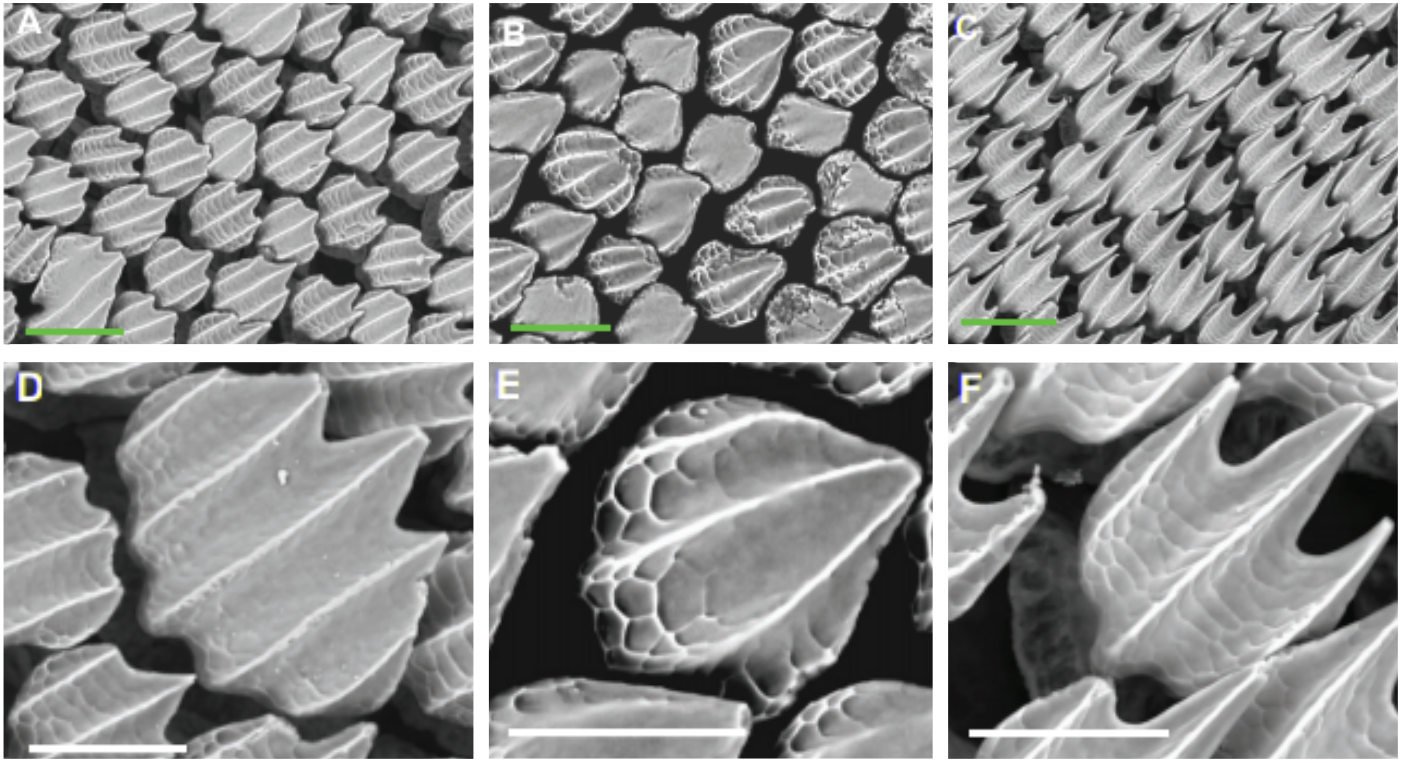
\includegraphics[width=12cm]{images/Scales2.png}
\caption{Shark scale samples taken from the head (A, D), the dorsal fin (B, E), and the anal fin (C, F) of a Mako shark. Green scale bars are \SI{200}{\mu m}; white scale bars are \SI{100}{\mu m}. Image adapted from \cite{wen2014}.}
\label{figure:scalesExample}
\end{figure}

However, riblets are one of many features that are present on shark scales (see Figure \ref{figure:scalesExample}). Through observation of the surface it is clear that the scales are very three-dimensional and variable in geometry between different shark species and location on the shark \citep{fletcher2014phd}. Some shark species have scales with no riblets, loosely interlocking scales, and variable angles of attack \citep{fletcher2014phd}. The dermis, of which scales are embedded, is known to be flexible, but the effect of this on the flow is not yet well understood \citep{wen2014}. The limited amount of work that has been carried out on shark scale surfaces is much more contradictory than similar experiments on riblets. This is due to variations in the scale geometry, replication errors, and experimental conditions. In addition to this, the most common experimental techniques are limited by the use of force balances, reducing the complexity of the flow to a single drag coefficient (further discussed in Section \ref{section:literatureReview}).


%Detailed flow structures have been investigated by either increasing the  size of the scales by several orders of magnitude \citep{lang2008} or carrying out expensive direct numerical simulation \citep{boomsma2015}.





\subsection{Research questions}

This project aims to determine the effect of scale geometry on the flow in order to identify why certain features have evolved and whether they can be optimised for drag reduction. In particular, the project aims to identify the effects of scale height and width, spacings between scales, the addition of riblets to smooth scales, and the effect of altering the angle of attack. This will be achieved by applying numerical parametric methods to a periodic array of scales. This will be validated against both a Large-Eddy Simulation (LES) and laboratory experiment utilising Laser Doppler Anemometry (LDA).
 
In addition to this the project will investigate the effect of applying scales to surfaces subject to separating flows. It has long been theorised that scales may prevent flow separation \citep{bechert1985} but current research is limited to analysis of large scale flow structures, rather than the flow features around individual scales. LES will be applied to a separating flow in order to quantify the differences between smooth and shark-skin surfaces. The results will be validated against a laboratory experiment using Particle Image Velocimetry (PIV). 

Despite the potential resolution of numerical methods, they have so far seen little use for resolving the flow around shark scales. This project will primarily use these techniques, validated against experimental data.

\subsection{Aim and Objectives}
\label{section:AandO}

There are two aims of this project; to investigate the influence of shark scale geometry on a fully developed flow, and to investigate the impact of scales on separating flows. Both of these aims will primarily concern the flow fields close to/around the scales. These will be achieved through completion of the following objectives:
\begin{itemize}
\itemsep0em

\item Identify experimental and numerical methods currently used in the literature and investigate their applicability to the current project.

\item Investigate potential software packages in terms of Computer-Aided Design (CAD) and Computational Fluid Dynamics (CFD). Carry out preliminary tests on potential software and identify which are most suitable. 

\item Carry out 3D LDA experiments for an array of scales in a channel.

\item Carry out a high resolution LES for the same array of scales and validate against LDA data. 

\item Validate a parametric RANS code against the LES/LDA data and carry out a parametric analysis on the effect of scale geometry on the fluid flow. 

\item Design and carry out laboratory (PIV) and numerical experiments (TBC) that can be used to investigate the influence of shark scales on separating flows.  

\end{itemize}

\section{Literature Review}
\label{section:literatureReview}
Most engineering and atmospheric flows are bounded by one or many surfaces. These take the form of external flows, such as the flow around cars and aircraft, and internal flows, such as through pipes and channels \citep{pope2001}. Boundary layers are formed as a fluid passes over a surface, whereby the surface-parallel fluid velocity converges to zero as the distance to the wall decreases. This no-slip condition causes a large contribution to the total drag force that impedes the motion of an object: \SI{50}{\%} of the drag that acts on a ship hull is due to this skin-friction \citep{perlin2016}. A typical boundary layer is presented in Figure \ref{figure:literatureReview:boundaryLayerRegions}, which splits the temporally averaged wall-parallel velocity into several different regions.
%
\begin{figure}[!b]
\centering
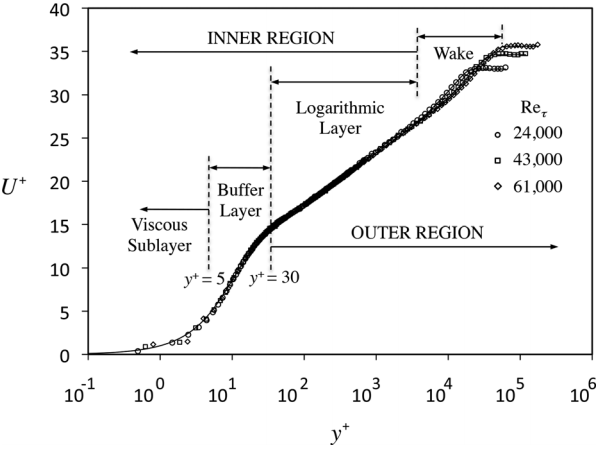
\includegraphics[width=10cm]{images/litReview/boundaryLayerRegions.png}
\caption{Regions of boundary layer from \cite{perlin2016} }
\label{figure:literatureReview:boundaryLayerRegions}
\end{figure}
%
Typically boundary layers are quantified using wall units, whereby variables are scaled using the fluid kinematic viscosity, $\nu$, and friction velocity, $u_\tau = \sqrt{\tau_w / \rho}$, where $\tau_w$ is the wall shear stress and $\rho$ is the fluid density. In wall units, the average velocity and distance are given by
\begin{equation}
U^+ = \frac{U}{u_\tau}, \hspace{1cm} y^+ = \frac{u_\tau y }{\nu}.
\end{equation}
By using this scaling the velocity profiles of many external and internal flows behave in the way indicated by Figure \ref{figure:literatureReview:boundaryLayerRegions}, whereby the boundary layer is split into external and internal regions. The inner region consists of a viscous sub-layer, whereby viscous forces dominate the near negligible inertial forces, a buffer layer, and a logarithmic layer. When in the viscous sub-layer the streamwise (wall-parallel) velocity of a fluid is proportional to the distance away from it, such that $U^+ = y^+$. This extends until $y^+ \approx 5$, at which point the production of turbulent kinetic energy rapidly increase until reaching its maximum in the buffer layer \citep{perlin2016}. The logarithmic region begins at $y^+ \approx 30$, at which point the streamwise velocity behaves like $U^+ = \kappa^{-1} \ln{y^+} + B$ where $\kappa \approx 0.4$ is the von Karmon constant and $B\approx 5$ is the intercept parameter \citep{pope2001}.

The outer layer blends the logarithmic region into the freestream velocity. The wake region, identified by Figure \ref{figure:literatureReview:boundaryLayerRegions}, deviates from the log-law and can cover a large amount of the boundary layer. For an external flow the wake region typically exists for $y/\delta > 0.2$ where $\delta$ is the boundary layer thickness, defined as the point at which the mean streamwise velocity is equal to \SI{99}{\%} of the freestream velocity, $U_\infty$. \cite{coles1956} postulated that this region can be defined by
\begin{equation}
\frac{U_\infty - U(y)}{u_\tau} = f \left( \frac{y}{\delta} \right),
\end{equation}
Several forms of $f(y/\delta)$ have been suggested, such as polynomial and trigonometric functions \citep{perlin2016}, which is generally more problem dependent than the logarithmic region (REFERENCE - POPE?). Generally the effect of surface roughness has no impact on the outer layers .. link to next section.

\subsection{Skin friction}
The two fundamental equations governing fluid flow are the continuity \eqref{equation:fundamentalEquations:continuity} and momentum \eqref{equation:fundamentalEquations:momentum} equations, derived by assuming incompressibility \citep{pope2001}:
\begin{equation}
\pdev{U_i}{x_i}=0,
\label{equation:fundamentalEquations:continuity}
\end{equation}
and
\begin{equation}
\Ddev{U_i}{t}
=
\pdev{\tau_{ij}}{x_i},
\label{equation:fundamentalEquations:momentum}
\end{equation}
where 
\begin{equation}
\tau_{ij}
=
-P\delta_{ij}
+
\nu\left( \pdev{U_i}{x_j}+\pdev{U_j}{x_i} \right),
\label{equation:fundamentalEquations:stressTensor}
\end{equation}
represents the stress tensor, $P = p/\rho$ represents the kinematic pressure, and $\nu$ represents the kinematic viscosity.

The mean flow equations can be derived by assuming the velocity and pressure variables can be decomposed into a fluctuating and mean component, such that

\begin{equation}
U_i = \langle U_i \rangle + u_i.
\label{equation:fundamentalEquations:ReynoldsDecomposition}
\end{equation}

The fundamental equations that dictate the behaviour of a Newtonian fluid is given by the three-component momentum equations and continuity equation:



Skin friction arises from wall-parallel momentum transfer and is directly related to the fluid velocity gradient at the wall surface:
\begin{equation}
\label{equation:literatureReview:wallShearStress}
u_\tau^2 = \frac{\tau_w}{\rho} = \left. \nu \frac{d U}{d y} \right\vert_{y=0}.
\end{equation}
The coefficient of friction normalises the shear stress with the dynamic pressure,
\begin{equation}
C_f = \frac{\tau_w}{\frac{1}{2} \rho U_b^2},
\end{equation}
where $U_b$ is the bulk fluid viscosity. For a statistically steady and fully developed channel flow the FIK identity \citep{fukagata2002} reduces to
\begin{equation}
\label{equation:literatureReview:FIK}
C_f = \frac{12}{Re_b} + 12 \int_0^\delta 2 \left(1 - \frac{y}{\delta} \right)\left( - \frac{\left< u'v' \right> }{4 U_b^2} \right) dy,
\end{equation}
where $\delta$ is half the channel height and $\left< u'v' \right>$ are the Reynolds stresses. For a laminar flow the second term of \eqref{equation:literatureReview:FIK} is zero. The second term is therefore the contribution to the wall shear stress that arises from turbulent fluctuations in the channel. 

- similar relationships can be derived 
- for pipes and open channel /flat palte flows
- these can include non-homogenous and time dependent terms
- Check some papers - what is the influence of turbulent structures on the flow




-is this important?
-equations to calculate it, where it is generated etc.
-FIK identity


\subsection{Coherent turbulent structures}
This section discusses the following:
\begin{itemize}
\item coherent structures in relation to wall-flows
\item streaks, bursts/ejections etc.
\item quadrant analysis as a method of detecting these features
\item contributions to Reynolds stresses / turbulent mixing and therefore drag

\end{itemize}

\subsection{Surface roughness}
The majority of real engineering problems are subject to surface roughness which is generally detrimental to efficiency. The first quantitative study on the effect of surface roughness was carried out by \cite{nikuradse1933} who applied different grain sizes of sand to a pipe flow and measured the resulting friction factor,
%
\begin{equation}
f \equiv \frac{\Delta p}{\Delta x} \frac{2D}{\rho U_b^2}
\end{equation}
%
where $\Delta p / \Delta x$ is the pressure drop per unit length, $D$ is the pipe diameter, $\rho$ is the fluid density and $U_b$ is the bulk velocity. Nikuradse observed that for both laminar and transitional flows surface roughness had little effect, and its effect on fully turbulent flows is dependent on the relative size of the roughness. To describe the effect of roughness three regimes were defined, based on the average roughness height, $k_s$:
%
$$\frac{k_s u_\tau}{\nu} < 5: \text{Hydraulically smooth,} $$
$$5 \leq \frac{k_s u_\tau}{\nu} \leq 70:	\text{transitionally rough,} $$
$$70 < \frac{k_s u_\tau}{\nu}:	\text{fully rough.}		$$
%
The hydraulically smooth regime occurs when the roughness elements do not protrude above the viscous sub-layer; In this case roughness has no effect. During the transitional stages roughness elements begin to protrude beyond the viscous sub layer, creating additional turbulent mixing and form drag on individual elements; both of these effects increase the friction factor relative to a smooth surface. The effect of roughness continues to grow until entering the fully-rough regime, at which point the friction factor is no longer a function of the Reynolds number.

In terms of the mean velocity profiles, roughness has the effect of shifting the logarithmic layer towards the wall such that the velocity behaves like
\begin{equation}
U^+ = \frac{1}{\kappa} \ln{y^+} + B - \Delta U^+,
\end{equation}
where $\Delta U^+$ represents the shift \citep{newhall2006}. Generally the gradient of the logarithmic region remains the same for both smooth and rough surfaces. In addition to this the outer layers of the boundary experience no change when subject to surface roughness, despite there being an increase to the boundary layer thickness, $\delta$ \citep{perlin2016}. However, the above description does not hold true for all types of roughness. In particular, the effect of shark-skin, and shark-skin inspired riblets, have a very different effect on the flow. These will be discussed in sections \ref{section:literatureReview:Riblets} and \ref{section:literatureReview:sharkScaleFluids}.

\subsection{Shark scales}
\label{section:literatureReview:sharkScales}
Sharks are the only surviving fishes that possess dermal denticles \citep{fletcher2014phd}. These small tooth-like structures erupt through soft skin tissue and are optimised for the prevention of abrasion, defence against parasites and the reduction of hydrodynamic drag \citep{fletcher2014phd}. An extensive range of dermal denticles are documented by \cite{reif1985}, highlighting the differences between shark species and the location of scales on the fishes. The study also indicates the complex features of real shark scales such as three dimensionality beneath the exposed scale, overlapping, diverging and converging riblets, variable angles of incidence, and the aerofoil-like shape of each scale with a smooth leading edge and a sharp trailing edge. These features can be observed in Figure \ref{figure:literatureReview:scaleVariabilityFletcher};
\begin{figure}[!h]
\centering
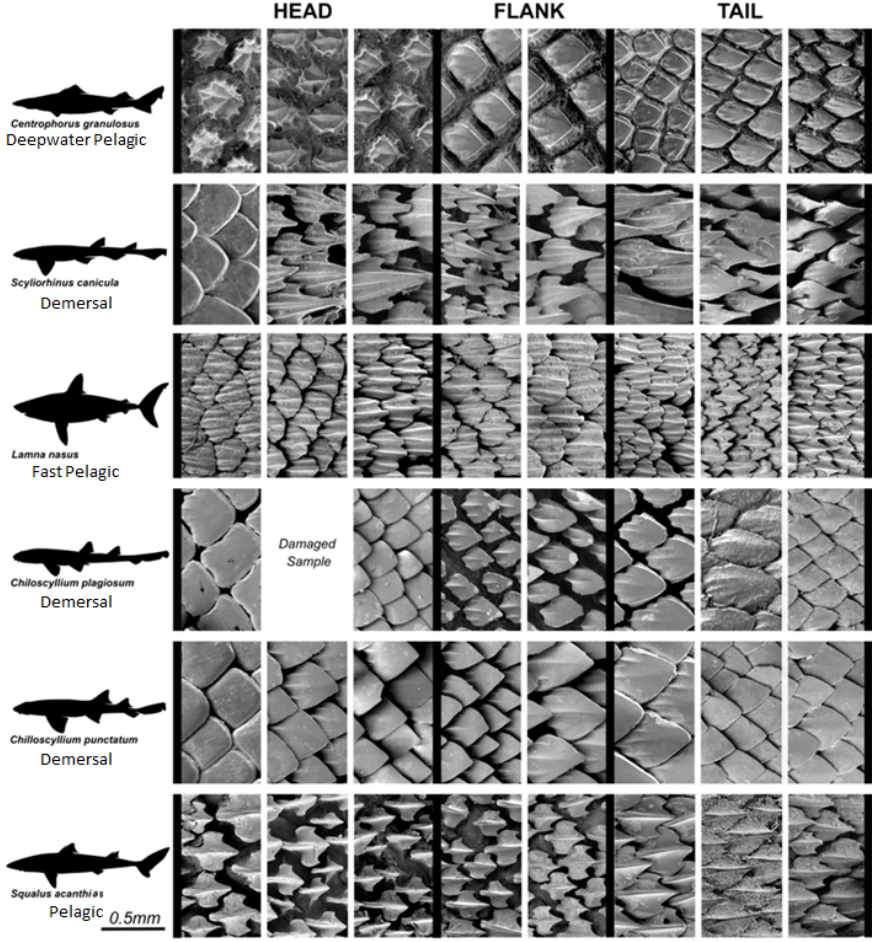
\includegraphics[width=14cm]{images/litReview/scaleVariabilityFletcher.png}
\caption{scale variability \citep{fletcher2014phd}}
\label{figure:literatureReview:scaleVariabilityFletcher}
\end{figure}
when considering even one species the scales can vary significantly when moving from the head to the tail. Take, for example, the \textit{Scyliorhinus canicula} (demersal ecology) samples; the scales on the head of the shark are tightly interlocking and rounded scales which quickly change to sharp, loosely interlocked, and ribletted scales on the sharks flank. The vast range of these features, and the variability between species, results in little understanding as to why many of these features exist. Hydrodynamical aspects have only been studied over the last few decades \citep{dean2010} and have only focussed on riblets, examples of which are most prominent on the fast pelagic samples of Figure \ref{figure:literatureReview:scaleVariabilityFletcher}. There have been research into the fluid dynamics of shark scales but there are many gaps and inconsistencies in the literature. These will be discussed in Section \ref{section:literatureReview:sharkScaleFluids}. 
%
\subsection{Riblets}
\label{section:literatureReview:Riblets}
 An extensive amount of work has been carried out on simplified, sharkskin-inspired, riblets which have been successful in reducing drag for open channel flows, closed channel flows and when applied to aerofoils \citep{bixler2013review}. These riblets are generally two-dimensional, whereby there is no variation in cross section in the streamwise direction. The most popular cross sectional shapes are blade like, sawtooth and scalloped although they are theorised to reduce drag in the same way. An example of blade-like riblets is presented in Figure \ref{figure:literatureReview:bladeRiblets}, and when compared to the denticle samples of Figure \ref{figure:literatureReview:scaleVariabilityFletcher} it is clear that the intricate details are lost.
%
\begin{figure}[!t]
\centering
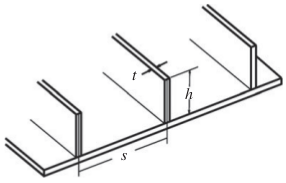
\includegraphics[width=8cm]{images/bladeRiblets.png}
\caption{Blade riblets from \cite{dean2010}}
\label{figure:literatureReview:bladeRiblets}
\end{figure} 
%
Figure \ref{figure:literatureReview:ribletPerformanceRegions} indicates three operating regions for the performance of a typical ribletted surface, whereby the difference in wall shear stress is plotted against the dimensionless riblet spacing, $s^+ = u_\tau s / \nu$.
%
\begin{figure}[!b]
\centering
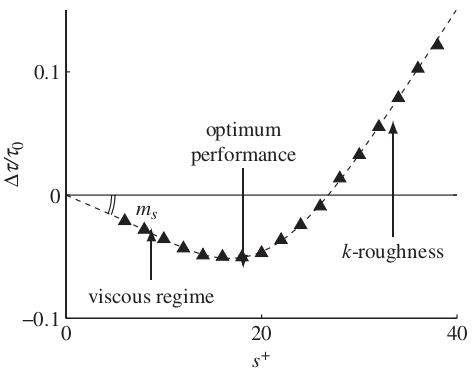
\includegraphics[width=8cm]{images/litReview/ribletPerformanceRegions.png}
\caption{Typical behaviour of riblets, from \cite{garcia2011}}
\label{figure:literatureReview:ribletPerformanceRegions}
\end{figure}
%
The viscous regime exists for riblets with a spacing of $s^+  \lesssim 15$ whereby the drag reduction scales linearly with spacing. The riblets act to impede cross-flow leading to a reduced susceptibility to secondary motion and therefore reduced turbulent mixing \citep{boomsma2015}. 


friction drag equation .... need some evidence that increasing mixing DOES increase drag ... 

look for Fukagata paper





The drag reduction process can be explained 


In order to investigate the drag reducing effect of riblets 

Typically, the drag reducing effect of riblets is studied by using a flat plate, mounted to a force balance. The drag force acting on the plate is recorded over a range of flow rates. 

the dimensionless riblet spacing is varied by varying the flow rate (Utau) rather than the physical spacing. 

Subsequently the plot of Figure \ref{figure:literatureReview:ribletPerformanceRegions} is given.

3 regions are present:
in the viscous regime the drag reduction, tau/tau0 is proportional to the riblet height. 

The DR occurs due to the restrictions on cross-stream motion that would otherwise lead to an increase in turbulent mixing. 

\vspace{5cm}
NEW PAPERS:\\
\citep{wei2005}: 	investiagates use of Clauser method for skin friction\\
\citep{atkin2016}:	investiagates staggered cavities using LDA and HWA - finds DR for some. Plots skin friction and vel. profiles.\\
\citep{tang1993}:	riblets, HWA and visuals, plots profiles, does quadrant analysis etc.\\
\citep{choi1989}: similar to above ..?\\

\vspace{5cm}



\newpage






- get an image and show a general curve
		-	first part is at width of ~ 0 i.e very low Reynolds number
						in this case DR scales linearly with height
						this is due to the impeding of cross-stream motion, that would lead to turbulent mixing and increase shearing  

- how do they work?
- key parameters?
- r
 
 \newpage
 

Drag reduction is achieved by 

\cite{dean2010} describes the drag reduction process as the lifting of cross-stream, high speed, vortices away from the wall whereby the high shear stresses associated with which only act at the riblet tips.


While vortices are introduced in-between riblets they are restricted by the riblet spacing, therefore reducing both shear stresses acting on the riblet valleys and the flow Reynolds stresses, both of which contribute to drag.

The riblets also act to impede the translation of secondary vortices, reducing vortex entanglement and ejection into the outer boundary layers. These effects are known to be reliant on the geometry of the riblet cross section: Riblets must protrude above the viscous sub-layer if vortices are to be impeded, and they must also be smaller than the near-wall vortices or else their motion will not be restricted \citep{dean2010}. 
 
 -Talk about relative size of scales! 
 
 - Introduce s+ but also other length scales such as A+ ...
 - Here we can introduce dimensionless parameters
 
 
 
  These effects have been visualised through the use of smoke-wire techniques \citep{lee2001}, PIV \citep{lee2008} and numerical methods \citep{goldstein1995}. Figure \ref{figure:literatureReview:smokeWireVisualisation} highlights the effect of scalloped riblets, whereby 
  The smoke-wire visualisations of \cite{lee2001} 
  
\begin{figure}[!t]
\centering
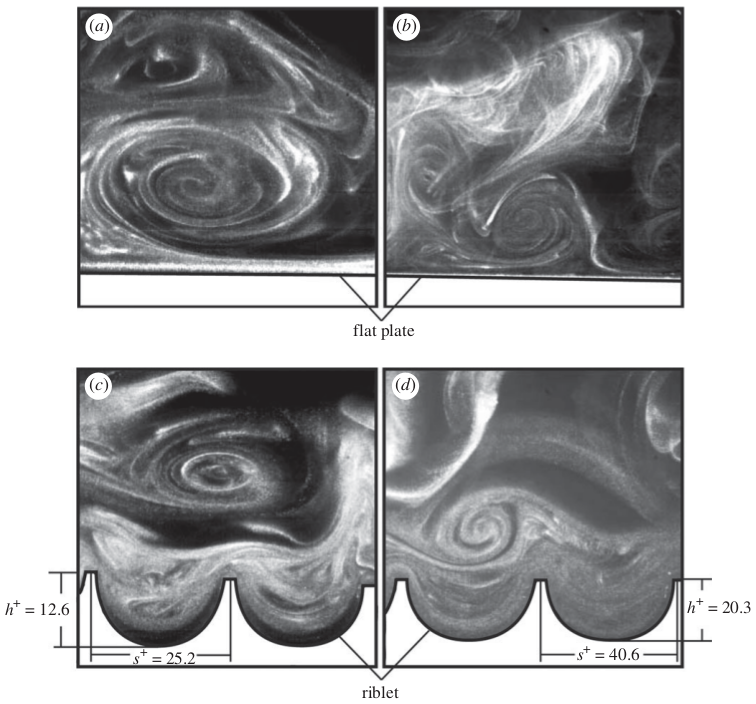
\includegraphics[width=12cm]{images/smokeWireVisualisation.png}
\caption{Smoke wire visualisation of \cite{lee2001}}
\label{figure:literatureReview:smokeWireVisualisation}
\end{figure}
 
 
 
 
  The literature is in general agreement that the optimal riblet spacing is $s^+ =  u_\tau s/\nu \sim 15$ where $s$ is the spacing between riblets, $u_\tau$ is the friction velocity of the flow without riblets and $\nu$ is the fluid viscosity.

\begin{table}[!t]
\scriptsize
\centering
\caption{Summary of experimental literature concerning the application of riblets to open channel flows. Adapted from \cite{bixler2013review}.}
\label{table:OpenChannelRiblet}
\begin{tabular}{|l|l|l|c|l|}
\hline
& & & & \\
\small Design                                                          & \small Confirguration                                            & \small Material                                              &  \multicolumn{1}{|l|}{\small Maximum Drag} &\small  Reference \\
& & & \multicolumn{1}{|l|}{\small Reduction} & \\
\hline

Sawtooth                                                               & Continuous                                                       & Polymer                                                      & 8\%                                        &   \citep{reidy1988}   \\
Sawtooth                                                               & Continuous                                                       & Vinyl                                                        & 9\%                                        &    \citep{rohr1992}  \\
Sawtooth                                                               & Continuous                                                       & Vinyl                                                        & 6\%                                        &   \citep{walsh1990}   \\
Sawtooth                                                               & Continuous                                                       & Vinyl                                                        & 9\%                                       &    \citep{neumann1991}  \\
\begin{tabular}[c]{@{}l@{}}Blade, Sawtooth\\ \& Scalloped\end{tabular} & Continuous                                                       & Brass                                                        & 9.9\%                                      &  \citep{bechert1997}    \\
Blade                                                                  & \begin{tabular}[c]{@{}l@{}}Staggered\\ \& Segmented\end{tabular} & Brass                                                        & 7\%                                        &    \citep{bechert2000}  \\
Blade                                                                  & \begin{tabular}[c]{@{}l@{}}Staggered\\ \& Segmented\end{tabular} & Epoxy                                                        & 7\%                                        &    \citep{bechert2000}  \\
Blade                                                                  & Continuous                                                       & \begin{tabular}[c]{@{}l@{}}Titanium \&\\ Nickel\end{tabular} & 4.9\%                                      &    \citep{buttner2011}  \\
Sawtooth                                                               & Continuous                                                       & Polyurethane                                                 & 7.6\%                                      &   \citep{gruneberger2011}   \\
Blade                                                                  & Continuous                                                       & \begin{tabular}[c]{@{}l@{}}Metal \&\\ Polymer\end{tabular}   & 8.5\%                                      &   \citep{wilkinson1988}   \\
Sawtooth, Scalloped & Continuous                                                       & \begin{tabular}[c]{@{}l@{}}Aluminium \&\\ Vinyl\end{tabular} & 8\%                                        &  \citep{walsh1982}  \\ \hline 
\end{tabular}
\end{table}

In terms of open channel flows there is good agreement between the available literature, whereby drag reduction reaches a maximum of 9.9\%, as indicated by Table \ref{table:OpenChannelRiblet}. However, from observation of Table \ref{table:ClosedChannelRiblet} there is less agreement when considering closed channel flows. These discrepancies are highlighted by \cite{bixler2013review} who indicates the restricting effect of channel height on cross-stream vortices. In the case of micro-sized channels the neighbouring wall effects become important. Sawtooth riblets have also been applied to a variety of different aerofoils over a range of Reynolds numbers, as summarised by Table \ref{table:AerofoilRiblets}. Again, drag reduction can be clearly achieved through the introduction of riblets.

\begin{table}[!b]
\centering
\caption{A summary of experimental literature concerning the application of riblets to closed channel flows. Adapted from \cite{bixler2013review}.}
\scriptsize
\label{table:ClosedChannelRiblet}
\begin{tabular}{|l|l|l|c|l|}
\hline
& & & & \\
\small Design                                                      & \small Configuration                                                               & \small Material                                                 &  \multicolumn{1}{|l|}{\small Maximum Drag} & \small Reference \\
& & & \multicolumn{1}{|l|}{\small Reduction} & \\
\hline

Blade                                                       & \begin{tabular}[|c|]{@{}l@{}}Aligned \& Segmented\end{tabular}               & Acrylic                                                  & 23\%                                                                                 &    \citep{jung2009}       \\
\begin{tabular}[|c|]{@{}l@{}}Blade \& Sawtooth\end{tabular} & \begin{tabular}[|c|]{@{}l@{}}Aligned \& Segmented,\\ Continuous\end{tabular} & \begin{tabular}[c]{@{}l@{}}Vinyl,\\ Acrylic\end{tabular} & 22\%                                                                                 &      \citep{bixler2013b}     \\
Sawtooth                                                    & Continuous                                                                   & Vinyl                                                    & 9\%                                                                                  &   \citep{rohr1992}        \\
Sawtooth                                                    & Continuous                                                                   & Polymer                                                  & 28\%                                                                                 &      \citep{reidy1988}     \\
Blade                                                       & \begin{tabular}[c]{@{}l@{}}Aligned \& Segmented,\\ Continuous\end{tabular} & Acrylic                                                  & 7\%                                                                                  &     \citep{bixler2013c}      \\
Blade                                                       & Continuous                                                                   & Polymer                                                  & 3\%                                                                                  &       \citep{nitschke1984}    \\
Sawtooth                                                    & Continuous                                                                   & Epoxy                                                    & 7\%                                                                                  &    \citep{enyutin1995}      \\
\hline
\end{tabular}
\end{table}

\begin{table}[!t]
\centering
\scriptsize
\caption{Summary of experimental literature concerning the application of riblets on aerofoils. Adapted from \cite{bixler2013review}.}
\label{table:AerofoilRiblets}
\begin{tabular}{|l|l|l|l|c|l|}
\hline
\begin{tabular}[c]{@{}l@{}}\small Reynolds\\\small Number\end{tabular}  &\small Foil Type                                                 & \begin{tabular}[c]{@{}l@{}}\small Location of\\\small  Trip (\% Chord\\ \small  Length)\end{tabular} & \begin{tabular}[c]{@{}l@{}} \small Angle of\\ \small  Attack\\ \small (degrees)\end{tabular} & \multicolumn{1}{|l|}{\begin{tabular}[c]{@{}l@{}} \small Maximum Drag\\ \small Reduction\end{tabular}} & \small Reference \\
\hline
17000                                                      & \begin{tabular}[c]{@{}l@{}}Symmetric,\\ Thin\end{tabular} & No Trip                                                                        & 0                                                                     & 4.3\%                                                                                &    \cite{han2003}       \\
250000                                                     & \begin{tabular}[c]{@{}l@{}}Symmetric,\\ Thin\end{tabular} & No Trip                                                                        & 0                                                                     & 13.3\%                                                                               &     \cite{caram1991}      \\
750000                                                     & Thin                                                      & 10\%                                                                           & 0-6                                                                   & 6\%                                                                                  &    \cite{sundaram1999}       \\
1000000                                                    & Symmetric                                                 & 10\%                                                                           & 0-6                                                                   & 13\%                                                                                 &   \cite{sundaram1996}        \\
1000000                                                    & Thin                                                      & 5\%                                                                            & 0                                                                     & 14\%                                                                                 &     \cite{subaschandar1999}      \\
1000000                                                    & Thick                                                     & No Trip                                                                        & 0                                                                     & 5\%                                                                                  &     \cite{wetzel1996}      \\
\begin{tabular}[c]{@{}l@{}}1000000\\ -1850000\end{tabular} & Thick                                                     & No Trip                                                                        & 0                                                                     & 5\%                                                                                  &      \cite{sareen2011}     \\
3000000                                                    & Thick                                                     & 6\%                                                                            & -0.5-1                                                                & 10\%                                                                                 &    \cite{viswanath1995}       \\
3300000                                                    & Thin                                                      & No Trip                                                                        & 0                                                                     & 3.3\%                                                                                &     \cite{coustols1990}      \\
\begin{tabular}[c]{@{}l@{}}2000000\\ -6000000\end{tabular} & \begin{tabular}[c]{@{}l@{}}Symmetric,\\ Thin\end{tabular} & 5\%                                                                            & 0                                                                     & 7\%                                                                                  &   \cite{bixler2013review}    \\
\hline   
\end{tabular}
\end{table}


The effect of riblets has also been captured using numerical techniques. \cite{choi1993} and \cite{chu1993} were among the first to investigate riblets using DNS methods, whereby high order turbulence statistics were extracted with good agreement with experimental data, achieving a reduction in drag of 6\%. \cite{goldstein1995} made use of immersed boundary methods to investigate the damping of cross-flow velocity fluctuations, achieving a drag reduction of 4\%. \cite{strand2011} uses a similar code to investigate the growth of turbulent spots in a developing boundary layer, making comparisons between ribletted and smooth surfaces. Three dimensional riblets have also been investigated using numerical techniques. \cite{martin2016a,martin2016b} use large eddy simulation to investigate segmented riblets concluding that three dimensional riblets are detrimental to drag reduction. The authors suggest that the three dimensionality of real shark scales is detrimental to drag reduction due to the segmented riblets. However, the model greatly simplifies the sharkskin geometry.

\newpage

\vspace{2cm}
-	Then talk about skin friction - we have an equation for it ...

-streaks and coherent structures
-APG vs ZPG etc. 

-	shark skin
	-	riblets - section as is
	-	sharkskin	-	what has been done here ....
					-	NOTE:	difficulties in exp. range ... s+ clearly doesn't match for sharks vs riblets ...

\vspace{2cm}


\newpage

New Structure:\\
intro:-	Shark skin has been studied for blah blah years, large documents on fossils by ...\\
-	This is what they look like and their theorised purpose is :  look at Fletcher ..\\
-	Give a diagram and show the flow direction - also show variety of scales\\
-	Then talk about riblets ...\\
-	Can go into more depth - talk about numerical methods in more detail, and get diagrams of different shapes, and get some graphs - show the important equations/dimensionless quantities. Also provide diagrams of how vortices are lifted away from riblets.\\
-	then provide our tables etc ...\\
-	Close the section by talking about how simplified these 'scales' are and introduce the next section...\\
****	Find the paper on tomo-PIV.\\
-	next section: experiments on real shark scales ... \\
-	Introduce with Becheret (?) experiments and talk about how he theorised they may work .. \\
-	Briefly go through each key paper, as we have done already. Talk about how, unlike the large amounts of work on riblets, nobody has actually looked into the flow profiles (or at least very few).

\newpage

\subsection{Fluid dynamic experiments concerning shark scales }
\label{section:literatureReview:sharkScaleFluids}




Sharkskin is comprised of small tooth-like structures called dermal denticles which are optimised to prevent abrasion, defence from parasites and reduce hydrodynamic drag \citep{fletcher2014}. The hydrodynamic properties of sharkskin is of interest to engineers due to the industrial applications of drag reduction, such as the transport of oil and gas and the design of aircraft and ships \citep{dean2010}. An extensive amount of work has been carried out on simplified, sharkskin-inspired, riblets which have been successful in reducing drag for open channel flows, closed channel flows and application to aerofoils \citep{bixler2013review}. These riblets are generally two-dimensional, whereby there is no variation in cross section in the streamwise direction. The most popular cross sectional shapes are blade like, sawtooth and scalloped although they are theorised to reduce drag in the same way. \cite{dean2010} describes the drag reduction process as the lifting of cross-stream, high speed, vortices away from the wall whereby the high shear stresses associated with which only act at the riblet tips. While vortices are introduced in-between riblets they are restricted by the riblet spacing, therefore reducing both shear stresses acting on the riblet valleys and the flow Reynolds stresses, both of which contribute to drag. The riblets also act to impede the translation of secondary vortices, reducing vortex entanglement and ejection into the outer boundary layers. These effects are known to be reliant on the geometry of the riblet cross section: Riblets must protrude above the viscous sub-layer if vortices are to be impeded, and they must also be smaller than the near-wall vortices or else their motion will not be restricted \citep{dean2010}. These effects have been visualised through the use of smoke-wire techniques \citep{lee2001}, PIV \citep{lee2008} and numerical methods \citep{goldstein1995}. The literature is in general agreement that the optimal riblet spacing is $s^+ =  u_\tau s/\nu \sim 15$ where $s$ is the spacing between riblets, $u_\tau$ is the friction velocity of the flow without riblets and $\nu$ is the fluid viscosity.

\begin{table}[!t]
\scriptsize
\centering
\caption{Summary of experimental literature concerning the application of riblets to open channel flows. Adapted from \cite{bixler2013review}.}
\label{table:OpenChannelRiblet}
\begin{tabular}{|l|l|l|c|l|}
\hline
& & & & \\
\small Design                                                          & \small Confirguration                                            & \small Material                                              &  \multicolumn{1}{|l|}{\small Maximum Drag} &\small  Reference \\
& & & \multicolumn{1}{|l|}{\small Reduction} & \\
\hline

Sawtooth                                                               & Continuous                                                       & Polymer                                                      & 8\%                                        &   \citep{reidy1988}   \\
Sawtooth                                                               & Continuous                                                       & Vinyl                                                        & 9\%                                        &    \citep{rohr1992}  \\
Sawtooth                                                               & Continuous                                                       & Vinyl                                                        & 6\%                                        &   \citep{walsh1990}   \\
Sawtooth                                                               & Continuous                                                       & Vinyl                                                        & 9\%                                       &    \citep{neumann1991}  \\
\begin{tabular}[c]{@{}l@{}}Blade, Sawtooth\\ \& Scalloped\end{tabular} & Continuous                                                       & Brass                                                        & 9.9\%                                      &  \citep{bechert1997}    \\
Blade                                                                  & \begin{tabular}[c]{@{}l@{}}Staggered\\ \& Segmented\end{tabular} & Brass                                                        & 7\%                                        &    \citep{bechert2000}  \\
Blade                                                                  & \begin{tabular}[c]{@{}l@{}}Staggered\\ \& Segmented\end{tabular} & Epoxy                                                        & 7\%                                        &    \citep{bechert2000}  \\
Blade                                                                  & Continuous                                                       & \begin{tabular}[c]{@{}l@{}}Titanium \&\\ Nickel\end{tabular} & 4.9\%                                      &    \citep{buttner2011}  \\
Sawtooth                                                               & Continuous                                                       & Polyurethane                                                 & 7.6\%                                      &   \citep{gruneberger2011}   \\
Blade                                                                  & Continuous                                                       & \begin{tabular}[c]{@{}l@{}}Metal \&\\ Polymer\end{tabular}   & 8.5\%                                      &   \citep{wilkinson1988}   \\
Sawtooth, Scalloped & Continuous                                                       & \begin{tabular}[c]{@{}l@{}}Aluminium \&\\ Vinyl\end{tabular} & 8\%                                        &  \citep{walsh1982}  \\ \hline 
\end{tabular}
\end{table}

In terms of open channel flows there is good agreement between the available literature, whereby drag reduction reaches a maximum of 9.9\%, as indicated by Table \ref{table:OpenChannelRiblet}. However, from observation of Table \ref{table:ClosedChannelRiblet} there is less agreement when considering closed channel flows. These discrepancies are highlighted by \cite{bixler2013review} who indicates the restricting effect of channel height on cross-stream vortices. In the case of micro-sized channels the neighbouring wall effects become important. Sawtooth riblets have also been applied to a variety of different aerofoils over a range of Reynolds numbers, as summarised by Table \ref{table:AerofoilRiblets}. Again, drag reduction can be clearly achieved through the introduction of riblets.

\begin{table}[!b]
\centering
\caption{A summary of experimental literature concerning the application of riblets to closed channel flows. Adapted from \cite{bixler2013review}.}
\scriptsize
\label{table:ClosedChannelRiblet}
\begin{tabular}{|l|l|l|c|l|}
\hline
& & & & \\
\small Design                                                      & \small Configuration                                                               & \small Material                                                 &  \multicolumn{1}{|l|}{\small Maximum Drag} & \small Reference \\
& & & \multicolumn{1}{|l|}{\small Reduction} & \\
\hline

Blade                                                       & \begin{tabular}[|c|]{@{}l@{}}Aligned \& Segmented\end{tabular}               & Acrylic                                                  & 23\%                                                                                 &    \citep{jung2009}       \\
\begin{tabular}[|c|]{@{}l@{}}Blade \& Sawtooth\end{tabular} & \begin{tabular}[|c|]{@{}l@{}}Aligned \& Segmented,\\ Continuous\end{tabular} & \begin{tabular}[c]{@{}l@{}}Vinyl,\\ Acrylic\end{tabular} & 22\%                                                                                 &      \citep{bixler2013b}     \\
Sawtooth                                                    & Continuous                                                                   & Vinyl                                                    & 9\%                                                                                  &   \citep{rohr1992}        \\
Sawtooth                                                    & Continuous                                                                   & Polymer                                                  & 28\%                                                                                 &      \citep{reidy1988}     \\
Blade                                                       & \begin{tabular}[c]{@{}l@{}}Aligned \& Segmented,\\ Continuous\end{tabular} & Acrylic                                                  & 7\%                                                                                  &     \citep{bixler2013c}      \\
Blade                                                       & Continuous                                                                   & Polymer                                                  & 3\%                                                                                  &       \citep{nitschke1984}    \\
Sawtooth                                                    & Continuous                                                                   & Epoxy                                                    & 7\%                                                                                  &    \citep{enyutin1995}      \\
\hline
\end{tabular}
\end{table}

\begin{table}[!t]
\centering
\scriptsize
\caption{Summary of experimental literature concerning the application of riblets on aerofoils. Adapted from \cite{bixler2013review}.}
\label{table:AerofoilRiblets}
\begin{tabular}{|l|l|l|l|c|l|}
\hline
\begin{tabular}[c]{@{}l@{}}\small Reynolds\\\small Number\end{tabular}  &\small Foil Type                                                 & \begin{tabular}[c]{@{}l@{}}\small Location of\\\small  Trip (\% Chord\\ \small  Length)\end{tabular} & \begin{tabular}[c]{@{}l@{}} \small Angle of\\ \small  Attack\\ \small (degrees)\end{tabular} & \multicolumn{1}{|l|}{\begin{tabular}[c]{@{}l@{}} \small Maximum Drag\\ \small Reduction\end{tabular}} & \small Reference \\
\hline
17000                                                      & \begin{tabular}[c]{@{}l@{}}Symmetric,\\ Thin\end{tabular} & No Trip                                                                        & 0                                                                     & 4.3\%                                                                                &    \cite{han2003}       \\
250000                                                     & \begin{tabular}[c]{@{}l@{}}Symmetric,\\ Thin\end{tabular} & No Trip                                                                        & 0                                                                     & 13.3\%                                                                               &     \cite{caram1991}      \\
750000                                                     & Thin                                                      & 10\%                                                                           & 0-6                                                                   & 6\%                                                                                  &    \cite{sundaram1999}       \\
1000000                                                    & Symmetric                                                 & 10\%                                                                           & 0-6                                                                   & 13\%                                                                                 &   \cite{sundaram1996}        \\
1000000                                                    & Thin                                                      & 5\%                                                                            & 0                                                                     & 14\%                                                                                 &     \cite{subaschandar1999}      \\
1000000                                                    & Thick                                                     & No Trip                                                                        & 0                                                                     & 5\%                                                                                  &     \cite{wetzel1996}      \\
\begin{tabular}[c]{@{}l@{}}1000000\\ -1850000\end{tabular} & Thick                                                     & No Trip                                                                        & 0                                                                     & 5\%                                                                                  &      \cite{sareen2011}     \\
3000000                                                    & Thick                                                     & 6\%                                                                            & -0.5-1                                                                & 10\%                                                                                 &    \cite{viswanath1995}       \\
3300000                                                    & Thin                                                      & No Trip                                                                        & 0                                                                     & 3.3\%                                                                                &     \cite{coustols1990}      \\
\begin{tabular}[c]{@{}l@{}}2000000\\ -6000000\end{tabular} & \begin{tabular}[c]{@{}l@{}}Symmetric,\\ Thin\end{tabular} & 5\%                                                                            & 0                                                                     & 7\%                                                                                  &   \cite{bixler2013review}    \\
\hline   
\end{tabular}
\end{table}


The effect of riblets has also been captured using numerical techniques. \cite{choi1993} and \cite{chu1993} were among the first to investigate riblets using DNS methods, whereby high order turbulence statistics were extracted with good agreement with experimental data, achieving a reduction in drag of 6\%. \cite{goldstein1995} made use of immersed boundary methods to investigate the damping of cross-flow velocity fluctuations, achieving a drag reduction of 4\%. \cite{strand2011} uses a similar code to investigate the growth of turbulent spots in a developing boundary layer, making comparisons between ribletted and smooth surfaces. Three dimensional riblets have also been investigated using numerical techniques. \cite{martin2016a,martin2016b} use large eddy simulation to investigate segmented riblets concluding that three dimensional riblets are detrimental to drag reduction. The authors suggest that the three dimensionality of real shark scales is detrimental to drag reduction due to the segmented riblets. However, the model greatly simplifies the sharkskin geometry.


While much work has been carried out on streamwise riblets there are many aspects of shark scales which have been vastly simplified. An extensive range of dermal denticles are documented by \cite{reif1985}, highlighting the differences between shark species and the location of scales on the fishes. The study also indicates the complex features of real shark scales such as three dimensionality beneath the exposed scale, overlapping, diverging and converging riblets, variable angles of incidence, and the aerofoil-like shape of each scale with a smooth leading edge and a sharp trailing edge. The vast range of these features, and the variability between species, results in little understanding as to why many of these features exist.



 \cite{raschi1986} relates the swimming speed of sharks to the riblet spacing present on the scales of 8 shark species. Empirical methods are adopted to estimate the cruising and burst swimming speeds. For 6 of the 8 shark samples it is concluded that the riblet spacing and keel height are optimised for burst speeds rather than cruising. Conversely \cite{bechert1985} suggests that riblet spacings are suited for cruising speeds, although estimates a cruising speed of $5\ m/s$ compared to the $0.8\ m/s$ of \cite{raschi1986}.  \cite{bechert1985} investigates the drag reduction of both replicated shark skin (Mako and Silky Shark) and longitudinal riblets. The angle of attack of the scales is varied, hypothesising that scales can passively bristle in order to enhance turbulent mixing and in turn keep boundary layers attached. It is concluded that shear stresses increase with angle of attack, suggesting that perfectly interlocking scales are required for drag reduction. However, the experimental conditions are that of a flat plate whereas the scales of a shark are likely subject to adverse pressure gradients. The authors suggest that the increase in turbulent mixing reduces the susceptibility of flow separation thus ultimately reducing drag, although further experimental evidence is required to support this. 

Denticle distributions are also investigated by \cite{fletcher2014phd} who highlighting changes in scale width, riblet spacing and riblet angles over different shark species. A range of shark scales are fabricated using 3D printing and drag reduction is found even for smooth scales that lack riblets. The coefficient of friction is calculated from the fluid velocity profile, captured using LDA. More common methods of measuring drag reduction are through the use of force balances for open channels, or calculating pressure drops for closed channels \citep{bixler2013review}. \cite{fletcher2014phd} calculates a maximum drag reduction of 35\% for a 3D printed \textit{Lophosteus} scale and 33.5\% for a \textit{Loganellia} sample, a smooth scale with no riblets.

Shark scales have also been fabricated by \cite{chen2014} who investigate both anti-fouling characteristics and drag reduction, comparing results to that of groove-like riblets. A bio-replication process is adopted to create a shark-skin surface. In this case, the \textit{Carcharhinus Brachyurous} sample is pretreated and a female die created using vacuum casting methods. Replication error is reduced to just 2\%. It is found that shark scales both enhance drag reduction ($\sim12\%$) and prevent fouling over the ribletted surface. However, little explanation is provided as to the possible mechanisms leading to such. It is suggested that the shark scale angle of attack and hydrophobicity could lead to these results. A similar technique is adopted by \cite{zhao2012} who achieves a maximum replication error of 7\%. The hydrophobic properties of the replicated surface are investigated, finding a significant increase in contact angle when compared to a smooth plate. A drag reduction of 18\% is achieved at the lowest velocity measured, which then reduces to a local minimum, raising to a local maximum and then reduces to its minimum value at the highest fluid velocity. This curve is particularly strange due to the two turning points in the velocity range tested. Without support from other literature this difference raises questions about the validity of the experimental techniques. \cite{zhang2011b} uses the same printing technology on a \textit{Isurus oxyrinchus} sample. Drag reduction is compared for a ribletted surface, sharkskin replica and a sharkskin replica with non-long polymer chains attached to the surface. a maximum drag reduction of 8\% is achieved for the sharkskin replica which increases to 24\% when the polymer is added. \cite{luo2015} makes use of both CFD and experimental techniques to investigate the drag reduction of moulded shark scales, although little detail is presented explaining either of the adopted methods. Reasonable drag reduction profiles are presented achieving a maximum of 12\%. Numerically the results appear far less convincing due to the poor documentation of the solver and models used.

Despite the popularity of moulding shark scale surfaces there are issues concerning the three-dimensionality being well replicated. Authors such as \cite{chen2014} indicate a small margin of error but use a tightly interlocking shark scale surface. It is known that cavities exist underneath many scale surfaces which cannot currently be replicated using moulds. An alternative technique is to apply samples of shark skin directly to flat plates and foils, removing the errors associated with replication. This is achieved by \cite{lang2014} who applies the skin of a shortfin mako shark to a NACA aerofoil to investigate boundary layer separation. Evidence is presented indicating the boundary layer control mechanisms of bristling scales.
However, this experimental technique is difficult to replicate due to the uncertainties regarding the shark skin sample. Not only this, but the scaling parameters are not of the same order of magnitude of a swimming shark due to the limitations of the experimental flow rate. Despite this, there is a clear reduction in backflow for the sharkskin surface. 

3D printing is rising in popularity although the technique is limited to an order of magnitude larger than the typical shortfin mako shark scale \citep{lang2008, fletcher2014phd, oeffner2012, wen2014, wen2015}.
\cite{wen2014,wen2015} print scales onto a flexible membrane in order to model the effect of flexibility. Contrary to the results of \citep{bechert1985} a drag reduction of $8.7\%$ is achieved by \cite{wen2014} when the scales are mounted to a flat plate. \cite{wen2015} explores the effect of denticle spacing using the same technique achieving a drag reduction of $10\%$ for linear, overlapping scales and $3\%$ for staggered, overlapped scales. However, these results show that drag reduction occurs at a much lower critical value of $s^+$ than longitudinal riblets and only three arrangements of denticles is tested. \cite{wen2014,wen2015} also apply these membranes to the low pressure surface of a flapping NACA aerofoil, hypothesising that the flexibility of the scales could have implications on thrust generation. Both studies conclude that the swimming speed of the self-propelling foil is increased when denticles are present but both the cost of transport (energy required per unit distance) and power required increased. The authors suggest that this is likely due to the poor representation of the flexible membrane to real shark skin where scales are more flexibly embedded into the dermis. However, it is suggested that dynamic experiments are more representative of shark skin and should be further investigated.

There is little literature available concerning the investigation of shark skin surfaces using numerical techniques. \cite{diez2015} models the flow over a mako shark using a roughness approximation to the shark skin in order to capture general flow properties. Parallels are made between the locations of different scale types and the flow conditions revealed by the numerical model. However, this simplification of the shark skin cannot reveal any related drag reduction mechanisms. \cite{zhang2011a} and \cite{luo2015}  use the RNG $k-\epsilon$ model to simulate the flow through a rectangular closed channel, one side of which consists of $\sim 30$ shark scales. A maximum drag reduction of $13\%$ is predicted using the model. Experimentally the same shark scales reduce drag by $9.5\%$. While these results are close the general trends do not agree: the numerical model suggests drag reduction increases with flow velocity while experimentally the opposite happens. A large reason for this could be due to the small channel height investigated: a height of 20 times the scale height is used, far larger than any experimental conditions. There is little detail present concerning either experimental or numerical model set up and no dimensionless quantities are stated making it hard to both replicate the results and compare them against other literature. Not only this but little explanation is given indicating the significance of the results presented. 

In contrast, a thorough DNS study is presented by \cite{boomsma2015} and \cite{boomsma2016} who simulate the flow over a simplified mako shark scale and parallel riblets, drawing comparisons between them and validating results against those of \cite{bechert1985}. A channel flow with both streamwise and cross stream periodicity is simulated using a stress-free boundary condition for the top surface. It is concluded that while riblets provide a drag reduction of $5.2\%$ shark scales increase drag by up to $50\%$ due to a large increase in turbulent mixing. These values are comparable to those of \cite{bechert1985} but contradict those of \cite{wen2014,wen2015}. \cite{boomsma2015} argues that the reason for this is due to the different experimental conditions of the authors. While \cite{boomsma2015} simulates a fully developed flow, this is unlikely to be the case experimentally. A large issue with the simulations carried out is the extensive computational power required, making further parametric studies infeasible. The simulations suggest an increase in turbulent mixing, detrimental to drag reduction, but \cite{bechert1985} argues that this can be beneficial for drag reduction in the presence of adverse pressure gradients. While the work of \cite{boomsma2015} is thorough the flow conditions of real sharks are not discussed.

Clearly there is discrepancy when considering the hydrodynamic experiments carried out on shark skin. Table \ref{table:SharkSkinExperiments} highlights these, indicating a range between a drag increase of 50\% and a decrease of 35\%. A large reason for this is the difficulties associated with replicating the scales: 3D printing is limited to a resolution of an order of magnitude greater than shark scales and moulding methods cannot capture the intricate details beneath the scale surface, thus limiting them to tightly interlocked scales. Another issue is that the experimental techniques are all limited by the use of a force balance whereby the flow manipulation of the scales cannot be investigated. LDA can be adopted to accurately measure the flow, but the current results of \cite{fletcher2014phd} show a much larger reduction in drag than any other techniques, even for scales without riblets. More data sets must be gathered to validate these results. Numerical methods have a much greater potential to analyse the flow field around the scales but the current work consists of either poorly documented RANS models or a very expensive DNS model. Parametric studies investigating scale size, geometry, spacing and overlapping effects could be incorporated into numerical models if a cheaper tool, such as LES/RANS, could be validated against the DNS data of \cite{boomsma2015}. However, the boundary conditions adopted by \cite{boomsma2015} are not appropriate to model the flow over a shark, as indicated by \cite{wen2014,wen2015}. Perhaps numerical or experimental investigations into the application of scales in adverse pressure gradients could provide a detailed analysis of the flow structures that cause the reduction in drag observed by \cite{wen2014,wen2015}.

\begin{table}[!t]
\scriptsize
\centering
\caption{Summary of experimental and numerical work concerning the drag reduction properties of shark skin}
\label{table:SharkSkinExperiments}
\begin{tabular}{|l|l|l|l|l|}
\hline
\small
Scale Type                           & \small \begin{tabular}[|c|]{@{}c@{}}Replication\\ Method\end{tabular} & \small  \begin{tabular}[|c|]{@{}c@{}}Experimental\\ Technique\end{tabular} & \small \begin{tabular}[|c|]{@{}c@{}}Max Drag\\ Reduction\end{tabular} & \small References \\

\hline
Mako, AOA 10 deg                     & Printing/casting                                             &  \begin{tabular}[l]{@{}l@{}}Wind tunnel \\ + balance  \end{tabular}                                     & -13\%                                              & \cite{bechert1985}                  \\
Mako, AOA 5 deg                      & Printing/casting                                                            & \begin{tabular}[l]{@{}l@{}}Wind tunnel \\ + balance  \end{tabular}        & -4\% & \cite{bechert1985}                             \\
Silky Shark                          & Printing/casting                                                            & \begin{tabular}[l]{@{}l@{}}Wind tunnel \\ + balance  \end{tabular}                                                                       & -1\%                                              & \cite{bechert1985}                             \\
\textit{Lophosteus}                  & 3D printing                                                  & \begin{tabular}[l]{@{}l@{}}Water flume \\ + LDA\end{tabular}                                                & 35\%                                                         & \cite{fletcher2014phd}                   \\
\textit{ \begin{tabular}[l]{@{}l@{}}Carcharhinus \\ Brachyurous \end{tabular} }    & Moulding                                                     & \begin{tabular}[l]{@{}l@{}}Water flume \\ + balance                                      \end{tabular} & 12\%                                                         & \cite{chen2014}                      \\
Not reported                         & Moulding                                                     & \begin{tabular}[l]{@{}l@{}}Water flume \\ + balance                                      \end{tabular} & 18.6\%                                                       & \cite{zhao2012}                      \\
\textit{Isurus Oxyrinchus}           & Moulding                                                     & \begin{tabular}[l]{@{}l@{}}Water flume \\ + balance                                      \end{tabular}                                      & 8\%                                                          & \cite{zhang2011a}                    \\
\begin{tabular}[l]{@{}l@{}} \textit{Isurus Oxyrinchus} \\ + polymer \end{tabular} & Moulding                                                            & \begin{tabular}[l]{@{}l@{}}Water flume \\ + balance                                      \end{tabular}                                      & 24\%                                                         & \cite{zhang2011a}                             \\
Not reported                         & Moulding                                                     & \begin{tabular}[l]{@{}l@{}}Water flume \\ + balance                                      \end{tabular}                                      & 12\%                                                         & \cite{luo2015}                      \\
\textit{Carcharhinus leucas}         & Moulding                                                     & \begin{tabular}[l]{@{}l@{}}Water flume \\ + balance                                      \end{tabular}                                      & 12\%                                                         & \cite{luo2015b}                     \\
\begin{tabular}[l]{@{}l@{}} \textit{Carcharhinus leucas} \\ + stretched \end{tabular}                      & Moulding                                                            & \begin{tabular}[l]{@{}l@{}}Water flume \\ + balance                                      \end{tabular}                                      & 14\%                                                         & \cite{luo2015b} \\
Mako                                 & 3D printed                                                   & \begin{tabular}[l]{@{}l@{}}Water flume \\ + balance                                      \end{tabular}                                      & 8.7\%                                                        & \cite{wen2014}   \\
Mako                                 & 3D printed                                                   & \begin{tabular}[l]{@{}l@{}}Water flume \\ + balance                                      \end{tabular} & 10\%                                                         & \cite{wen2015}   \\
Not reported                         & Scanned + smoothed                                           & Numerical RANS                                                   & 13\%                                                         & \cite{zhang2011a}  \\
Not reported                         & Moulding                                                     & \begin{tabular}[l]{@{}l@{}}Water flume \\ + balance                                      \end{tabular} & 9.5\%                                                        & \cite{zhang2011a}        \\
Mako                                 & Scanned + smoothed                                           & Numerical DNS                                                    & -50\%                                                        & \cite{boomsma2015} 
\\
\hline    
\end{tabular}
\end{table}
\newpage

\section{Mathematical Modelling: Introduction to RANS and LES}
This section introduces the mathematical models adopted in the present work. Two different approaches are described: Reynolds Averaged Navier-Stokes and Large-Eddy-Simulation; both of which are derived from the same fundamental equations. 

\vspace{2cm}

- talk about different types of models: URANS, SAS DES etc ... Then specify a few specific models 

\vspace{2cm}

Structure:\\
-	Fundamental eq. and derivation of Reynolds Eq.\\
-	Turbulent viscosity hyp. + standard assumptions\\
-	Link this to development of RANS and the standard equations. - Derive these (for k)\\
-	** Give a description of available turbulence models (common ones) and a description of why they are not applicable.\\
Algebraic: mixing length (
...
Be more general: Suggest that generally adding more eq. resolves turbulence better but at an increased cost. 

\subsection{Fundamental equations}
The two fundamental equations governing fluid flow are the continuity \eqref{equation:fundamentalEquations:continuity} and momentum \eqref{equation:fundamentalEquations:momentum} equations, derived by assuming incompressibility \citep{pope2001}:
\begin{equation}
\pdev{U_i}{x_i}=0,
\label{equation:fundamentalEquations:continu}
\end{equation}
and
\begin{equation}
\Ddev{U_i}{t}
=
\pdev{\tau_{ij}}{x_i},
\label{equation:fundamentalEquations:mome}
\end{equation}
where 
\begin{equation}
\tau_{ij}
=
-P\delta_{ij}
+
\nu\left( \pdev{U_i}{x_j}+\pdev{U_j}{x_i} \right),
\label{equation:fundamentalEquations:stresr}
\end{equation}
represents the stress tensor. 

The mean flow equations can be derived by assuming the velocity and pressure variables can be decomposed into a fluctuating and mean component, such that

\begin{equation}
U_i = \langle U_i \rangle + u_i.
\label{equation:fundamentalEquations:Reynoltion}
\end{equation}

By substituting this form of $U_i$ into the continuity \eqref{equation:fundamentalEquations:continuity} equation we get
\begin{equation}
\pdev{\langle U_i\rangle}{x_i}=0,
\label{equation:fundamentalEquations:meanContinuity}
\end{equation}
and
\begin{equation}
\pdev{u_i}{x_i}=0.
\label{equation:fundamentalEquations:flucContinuity}
\end{equation}
By averaging the terms in the momentum equations we get
\begin{equation}
\left\langle \Ddev{U_i}{t} \right\rangle
=
-\pdev{\langle P \rangle}{x_i}
+
\nu
	\left(
	\pdev{\langle U_j \rangle}{x_i}
	+
	\pdev{\langle U_i \rangle}{x_j} 
	\right).
\label{equation:fundamentalEquations:averagedMom}
\end{equation}
The material derivative can be simplified by
\begin{equation}
\left\langle \Ddev{U_i}{t} \right\rangle
=
\left\langle
	\pdev{U_i}{t} + \pdev{U_i U_j}{x_i}
\right\rangle
=
\pdev{\langle U_i\rangle}{t}
+
\pdev{\langle U_i U_j\rangle}{x_i},
\end{equation}
\begin{align}
\langle U_i U_j\rangle 
&=
\langle
	(\langle U_i \rangle + u_i)(\langle U_i \rangle + u_i)
\rangle \\
&=
\langle
	\langle U_i \rangle \langle U_j \rangle
	+
	u_i \langle U_j \rangle
	+
	u_j \langle U_i \rangle
	+
	\langle u_i u_j \rangle
\rangle\\
&=
\langle U_i \rangle \langle U_j \rangle
+
\langle u_i u_j \rangle.
\end{align}
Therefore,
\begin{align}
\left\langle \Ddev{U_i}{t} \right\rangle
&=
\pdev{\langle U_i\rangle}{t} 
+
\pdev{\langle U_i\rangle \langle U_j\rangle}{x_i}
+
\pdev{\langle u_i u_j\rangle}{x_i},\\
&=
\frac{\overline{D} \langle U_i \rangle }{ \overline{D} t}
+ 
\pdev{\langle u_i u_j\rangle}{x_i}
\end{align}
where $\overline{D}_t$ represents the mean material derivative. 

Substituting this back into \eqref{equation:fundamentalEquations:averagedMom} we result in the Reynolds equations \citep{pope2001}:
\begin{equation}
\frac{\overline{D} \langle U_i \rangle }{ \overline{D} t}
=
-\pdev{\langle P \rangle}{x_i}
+
\nu
	\left(
	\pdev{\langle U_j \rangle}{x_i}
	+
	\pdev{\langle U_i \rangle}{x_j} 
	\right)
+
\pdev{\langle u_i u_j\rangle}{x_i}.
\label{equation:fundamentalEquations:ReynoldsEquations}
\end{equation}
These equations are similar in appearance as the Navier-Stokes equations \eqref{equation:fundamentalEquations:momentum} but require information about the Reynolds stresses, $\langle u_i u_j \rangle$. This forms the basis of the RANS ideology, whereby \eqref{equation:fundamentalEquations:meanContinuity} and \eqref{equation:fundamentalEquations:ReynoldsEquations} are solved for $\langle U_i \rangle$ and $\langle P \rangle$ by modelling the Reynolds stresses. There have been many proposed models to close this system of equations with varying accuracy and expense. A widely adopted approach to modelling these stresses is the turbulent-viscosity hypothesis which assumes
\begin{equation}
\left< u_i u_j \right> = \frac{2}{3}k \delta_{ij} - \nu_T \left( 
	\pdev{\left< U_i \right>}{x_j} + \pdev{\left< U_j \right>}{x_i}	\right),
\end{equation}
where $\nu_T(\boldsymbol{x},t)$ is the turbulent viscosity, analogous to the molecular viscosity. Algebraic relationships for $\nu_T$ have been suggested, such that $\nu_T=l_m^2 \left| (\partial \left<U\right> / \partial y   \right|$, but these are reliant on the specification of the mixing length $l_m$. 

\begin{equation}
\nu_T = c k^{1/2} l_m = C_\mu k^2/\epsilon,
\end{equation}


\begin{equation}
\pdev{k}{t} + \left< U_i \right> \cdot \nabla k = -\nabla \cdot T_i' + \mathcal{P} - \epsilon 
\end{equation}

\begin{equation}
T_i' = \frac{1}{2} \left< u_i u_j u_j \right> + \left< u_i P' \right> - 2 \nu \left< u_j s_{ij} \right>.
\end{equation}
where $P'$ is the fluctuation component of the kinematic pressure. Further assumptions: the flux, $T_i'$ is modelled using gradient diffusion, i.e 
\begin{equation}
T_i' = -\frac{\nu_T}{\sigma_{k}} \nabla k,
\end{equation}
where the turbulent Prandtl number is generally taken as $\sigma_k=1$. This physically asserts that due to velocity and pressure fluctuations there is a flux of k down the gradient of k \citep{pope2001}.

The equation for epsilon is entirely empirical:
\begin{equation}
\pdev{\epsilon}{t}  + \left< U_i \right> \cdot \nabla \epsilon = \nabla \cdot \left( \frac{\nu_T}{\sigma_{\epsilon}} \nabla \epsilon \right) + C_{\epsilon 1} \frac{\mathcal{P} \epsilon}{k} - C_{\epsilon 2} \frac{\epsilon^2}{k}
\end{equation}
as is the one for omega .. 
\begin{equation}
\pdev{\omega}{t}  + \left< U_i \right> \cdot \nabla \omega = \nabla \cdot \left( \frac{\nu_T}{\sigma_{\omega}} \nabla \omega \right) + C_{\omega 1} \frac{\mathcal{P} \omega}{k} - C_{\omega 2} \omega^2
\end{equation}
By taking $\omega \equiv \epsilon /k$ and substituting into $\epsilon$ equation we get
\begin{equation}
\pdev{\omega}{t}  + \left< U_i \right> \cdot \nabla \omega = \nabla \cdot \left( \frac{\nu_T}{\sigma_{\epsilon}} \nabla \omega \right) + (C_{\varepsilon 1}-1) \frac{\mathcal{P} \omega}{k} - (C_{\varepsilon 2}-1) \omega^2 + \frac{2 \nu_T}{\sigma_\epsilon k}\nabla \omega \cdot \nabla k
\end{equation}

\newpage

\section{Channel Flow Experiments using Laser Doppler Anemometry}
As discussed in Section \ref{section:literatureReview}, little work has been carried out in analysing the fluid flow around shark scale surfaces; most work has focussed on the use of force balances which cannot measure velocity or pressure fields. While previous experiments have successfully measured drag reduction for shark scale surfaces they have not yet investigated the fluid dynamic features that are causing it. For this reason we choose to adopt Laser Doppler Anemometry (LDA) to measure a channel flow, with and without shark scales. While a channel flow does not replicate the complex flow fields around a shark, it allows comparison against a wide range of empirical and numerical literature data (in the case of smooth channels), and also ensures the results are applicable to a wide range of surface flows, such as boat hulls and pipe walls. In addition to this, understanding how shark scales behave in simple and controllable configurations will provide comparative data when investigating their effects on separating flows. This simplification also allows numerical models to exploit the periodicity of shark scale surfaces, greatly reducing the required computing power for numerical methods. 

This section details the preliminary experiments, the aim of which are to validate the experimental method and identify changes that must be made to future designs. Current rig designs are based on those of \cite{fletcher2014phd} who adopts 2D LDA (measuring streamwise and wall-normal components of velocity) to compare differences between 5 shark scale samples, in terms of velocity profiles and skin friction coefficients. These experiments make use of a recirculating flume with a removable flat plate (figure XX - Make image of the measurement section). This set up has a practical advantage since scale samples can be easily swapped. However, the present study requires comparison with numerical models, thus the experimental solutions are validated against the empirical law of the wall (reference) and literature data (find some, or do a RANS for it) for a fully developed channel flow. In addition to this the sensitivity to wall-normal spatial resolution and temporal averaging window are also assessed.

\subsection{Fundamentals of LDA}
LDA is a non-intrusive method of determining a fluids velocity by measuring the Doppler shift of laser light (reference the LDA book). There are several key components which can be split into two groups; an optical unit and a receiving unit. The optical unit generates and transmits a pair of laser beams for each velocity component and focusses them onto a small volume, with a typical width of \SI{100}{\mu m} (Reference). The two beams create a fringe pattern in the measurement volume, the spacing of which, $\Delta x$, is determined by the angle of intersection, $\alpha$, and the light wavelength, $\lambda$. This is demonstrated in Figure \ref{figure:experiments:fringePattern}, whereby a particle of velocity $\vect{u}_p$ passes through the fringing pattern created by the two beams $E_a$ and $E_b$. The two beams can be represented by 
%
\begin{figure}[!t]
\centering
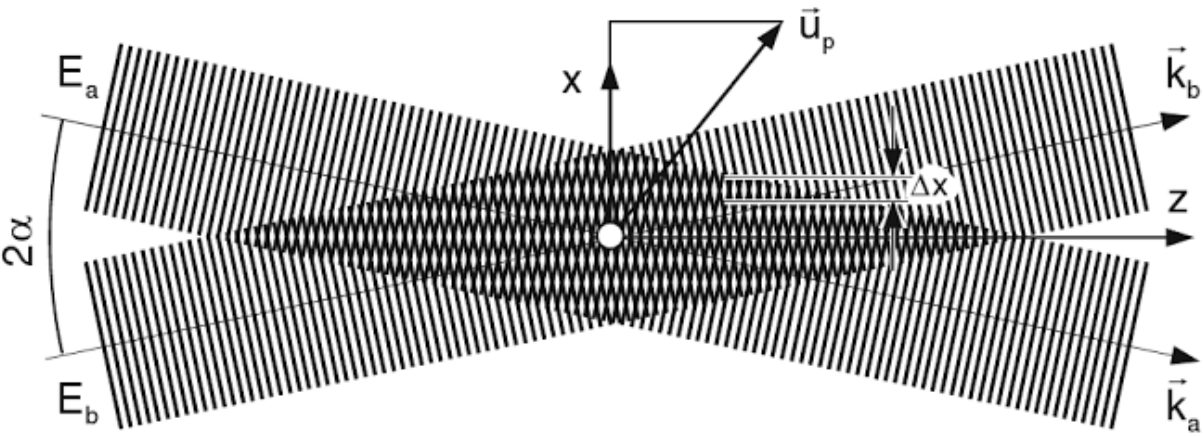
\includegraphics[width=10cm]{images/LDA_theoryImages/fringePattern.png}
\caption{Fringe pattern (LDA book reference)}
\label{figure:experiments:fringePattern}
\end{figure}
%
\begin{equation}
E_a = E_0 \cos {\left[ \omega_a t - k_a (z \cos{\alpha} - x \sin{\alpha} ) \right]},
\end{equation}
and
\begin{equation}
E_b = E_0 \cos{ \left[ \omega_b t - k_b (z \cos{\alpha} + x \sin{\alpha} ) \right]},
\end{equation}
where $E_0$ represents the wave amplitude, $\omega = 2 \pi / T$ the respective angular frequencies and $k = 2 \pi / \lambda$ the angular wavenumber. The wavelength is related to the speed of light by $c = \lambda f$ where $c$ represents the speed of light and $f$ represents the oscillation frequency. With some manipulation the $x$-component of the particle velocity is found to be directly related to both the fringe spacing and the shift in oscillation frequency as the particle passes through the fringes (Reference LDA book). The receiving components detect this change in frequency which is subsequently converted to an electrical signal and processed. In order to relate particle velocity to fluid velocity the flow is seeded with neutrally buoyant particles of \SI{40}{\mu m} diameter and it is assumed that these particles do not deviate from the fluid streamlines. 

The present work makes use of two-component LDA, whereby two pairs of beams are transmitted perpendicular to each other and of different wave lengths; one at $\lambda = $ \SI{514.51}{nm} (green light) and $\lambda = $ \SI{488}{nm} (blue light). The respective shifts in frequency are separated by the receiving unit in order to produce two velocity components. Particle velocities are also only recorded if a shift in frequency is observed by both beam pairs, thus the covariance of the two velocities can be analysed. 

Velocity biasing is a phenomena that must be considered when utilising LDA. Since velocities are only sampled when particles pass through the focal volume, the subsequent time series does not have a regular sampling interval. For this reason, high velocity fluctuations are measured more often than low velocity fluctuations which results in a bias towards higher velocities when calculating statistics such as means and standard deviations. The correction method of (reference) is adopted in the present work, whereby the means and standard deviations are normalised by the amount of time a particle resides in the focal volume, $\tau$. The temporal mean of a velocity component $u$ is therefore calculated by

\begin{equation}
\mu_u = \frac{\sum^N_{i=1} u_i \tau_i}{\sum^N_{i=1} \tau_i}, 
\end{equation}
and the standard deviation by
\begin{equation}
\sigma_u = \sqrt{\frac{\sum^N_{i=1} \tau_i (u_i - \mu_u)^2}{\sum^N_{i=1} \tau_i}}.
\end{equation}

\subsection{Experimental set up}
The experiments are carried out using a flat plate submerged in a recirculating flume (observed in Figure \ref{figure:experiments:setUp}).
%
\begin{figure}[!b]
\centering
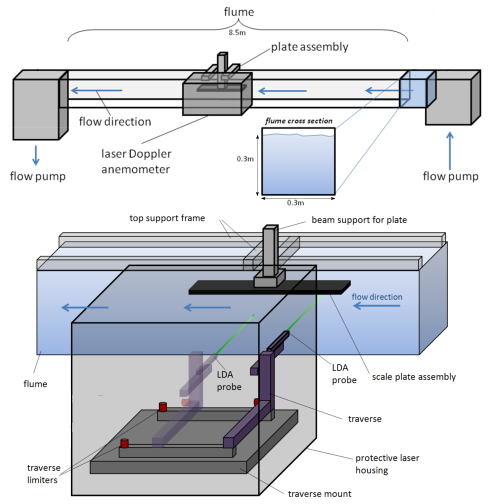
\includegraphics[width = 12cm]{images/LDA_theoryImages/expSetUp.png}
\caption{Rig design adapted from \cite{fletcher2014phd}}
\label{figure:experiments:setUp}
\end{figure}
%
The plate has the dimensions $L \times w \times h = 500 \times 100 \times 10 $ (mm) with semi-circular leading and trailing edges.


\vspace{5cm}
-water height 
-traverse and LDA set up (limits to traverse)
-pump settings
-filtering method
\vspace{2cm}



Several components are utilised in the current experimental set up; 





 For this reason, statistics such as means ans standard deviations are biased towards  
\\\\\\
 
Next - what do we do with the velocities : give equations for time averaging etc.
	-	also - mention two component LDA and configuration of the head
	-	




\vspace{2cm}

How?
	-	recirculating open channel flume with a submerged flat plate
	-	measured using LDA (2D and 3D)

Why?
	-	flat plate allows surface to be easily changed
	-	LDA is a highly accurate, non-intrusive method to extract 
		velocity data. It has been used to measure boundary layers 
		more successfully than other methods (?) and also used to 
		calculate coeffs of friction.
	-	LDA provides much more quantitative data than force balances
		for a given flow rate.



-	Fully developed
		-	how much does the flow change if it is not developed
-	time dependence
		-	how long do we need to average for for convergence
		-	what are the error estimates if we average for less time
			NOTE - Y+ VALUES ARE DIFFERENT FOR DIFF FLOW RATES
-	2D not 3D for prelim experiments
		-	Provides info for errors and exp design without 
			complications and additional run time
-	profiles
		-	Do we match law of the wall and other lit. with our rig
		-	Can we get reasonable estimates of skin friction coeff.
-	flow set up:	bluff body method
		-	Does this mess with the flow?
-	post-processing
		-	Filtering method

Section split into three main parts: time Dep, space Dep, and profiles + skin friction estimates.

!!!!	The mechanism controlling vortex shedding from rectangular bluff bodies !!! - This paper suggests a St number of 1 and therefore a shedding frequency of roughly 5/4. 

\subsection{Methodology and Equipment}
FLUME:
	-	get design from GK or look at papers from Sorby
	-	need diagram of this
	-	get pump design	
			-	can't have velocity too low or high - gives a range of shark scale sizes and Re numbers
	-	describe plate and provide diagram
	-	LDA
		-how it works
		-how its set up (2D), coincidence mode
	-post processing
		-weighting for velocity bias
		-filtering
			-	3 filters are tested, GA, MA and PSF
					-	Breifly describe these ..
					-	Then put in some data  - use time dep 4hz 1mm Uy 
							-	RMS of this clearly shows dependency
							-	Reason for harshness of PSF is due to gradient terms - we have removed data, not replaced it. 
							-	likely to be same for MA ... events become relatively shorter compared to window size 
							- THEREFORE need to test against what happens when we replace spikes with local means. 
		-this is different for each of the tests ....

Fundamentals of LDA, Flume used, pump used, plate design, post-processing methods 
\subsubsection{Rig design}
-pump
-flume
-scale printing + plate
-plate design
-mounting of laser + traverse
\subsubsection{Post processing methods}
In order to identify poor data several filtering methods have been applied. The simplest of which is a global average filter, whereby 
\begin{equation}
\mu_\phi - 2 \sigma_\phi < \overline{\phi} < \mu_\phi + 2 \sigma_\phi,
\end{equation}
where 
\begin{equation}
\mu_\phi = \frac{1}{N} \sum^N_{i=1} \phi_i,
\end{equation}
is the temporal average, and
\begin{equation}
\sigma_\phi = \sqrt{\frac{1}{N} \sum^N_{i=1} (\phi_i - \mu_\phi)^2	} 
\end{equation}
is the standard deviation. The choice of $\pm 2 \sigma_\phi$ ensures that $\sim$95$\%$ of the probability distribution function of $\phi$ is captured by the filter. An alternative method is to apply a moving average over an averaging window, $W$, such that
\begin{equation}
\mu_{\phi,i} - 2 \sigma_{\phi,i} < \overline{\phi_i} < \mu_{\phi,i} + 2 \sigma_{\phi_i},
\end{equation}
where 
\begin{equation}
\mu_{\phi,i} = \frac{1}{N} \sum^{W/2}_{j=-W/2} \phi_j,
\end{equation}
is the temporal average, and
\begin{equation}
\sigma_{\phi,i} = \sqrt{\frac{1}{N} \sum^{W/2}_{j=-W/2} (\phi_j - \mu_{\phi,i})^2	} 
\end{equation}
\vspace{2cm}
The advantage of this method is that deviations in local mean are captured, leading to a less 'harsh' method for filtering. The phase space filtering method of (Reference) adopts a different approach, whereby the variable $\phi$ and its first and second order derivatives, $d \phi$ and $d^2 \phi$, are ...
-filtering
-weighting
-RMS, means, stresses etc
-skin friction
-law of the wall 
-
\subsection{Preliminary Results}
Split into three ...
\subsubsection{Time Dependence}
\begin{figure}
\centering
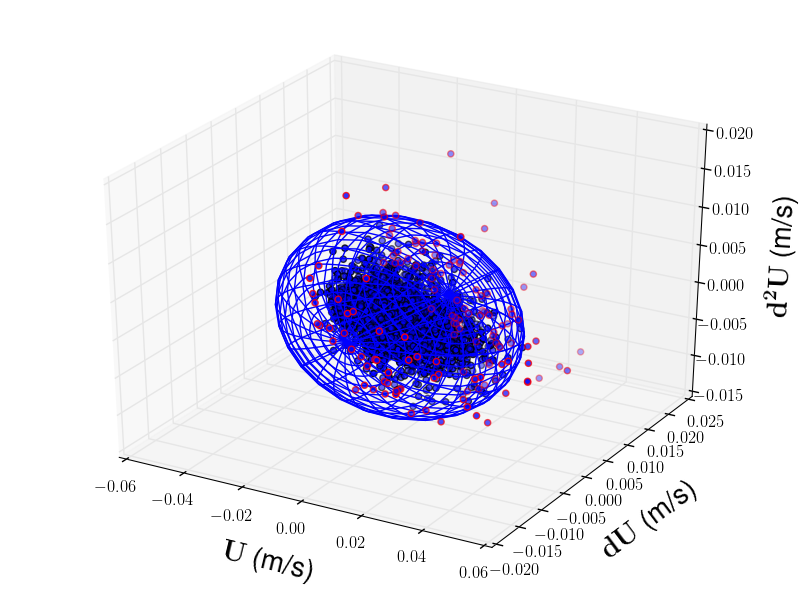
\includegraphics[width=12cm]{images/LDA_timeDependenceImages/4hz_x_400_z_1_Ux_phaseSpacePlot.png}\\
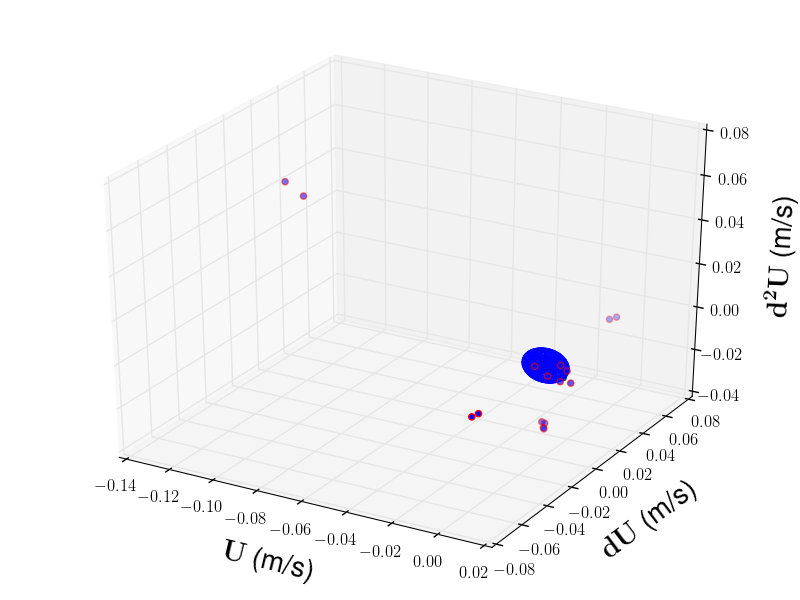
\includegraphics[width=12cm]{images/LDA_timeDependenceImages/4hz_x_400_z_1_Uy_phaseSpacePlot.png}\\
\caption{Example of phase space filter for $U_x$ (top) and $U_y$ (bottom).}
\label{figure:experiments:filteringExample}
\end{figure}

\begin{figure}
\centering
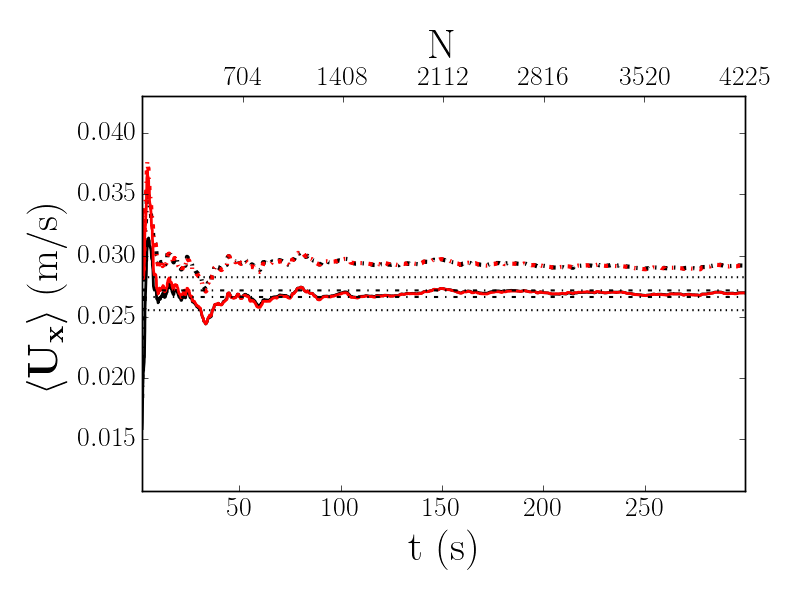
\includegraphics[width=7.5cm]{images/LDA_timeDependenceImages/4hz_x_400_z_1_MeanUx.png}\hfill
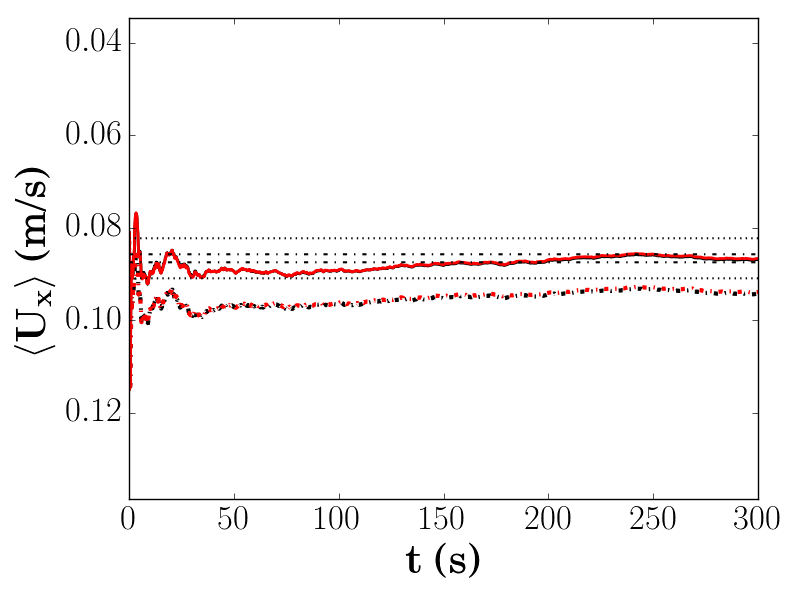
\includegraphics[width=7.5cm]{images/LDA_timeDependenceImages/8hz_x_400_z_1_MeanUx.png}\\
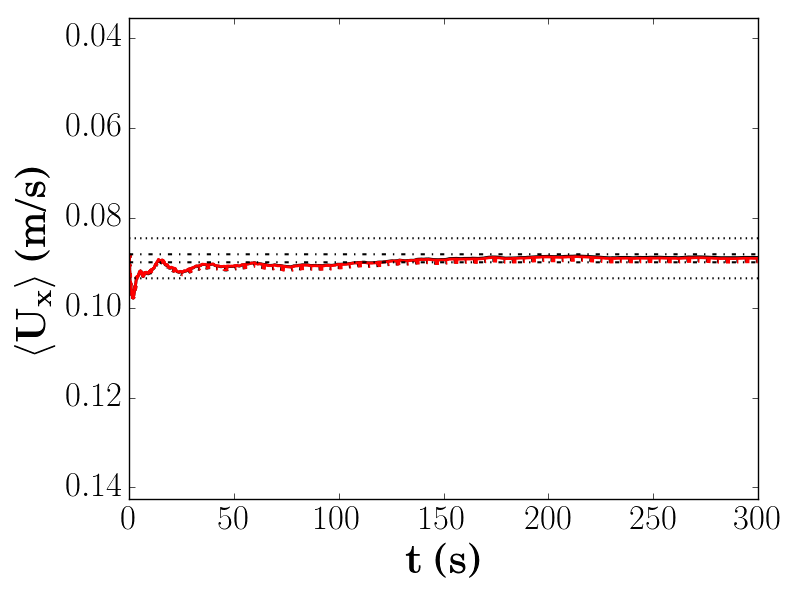
\includegraphics[width=7.5cm]{images/LDA_timeDependenceImages/4hz_x_400_z_15_MeanUx.png}\hfill
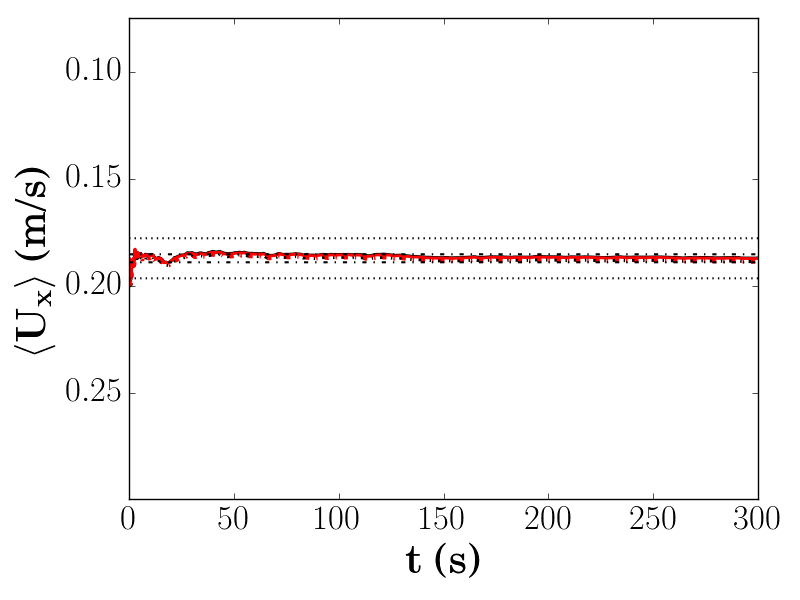
\includegraphics[width=7.5cm]{images/LDA_timeDependenceImages/8hz_x_400_z_15_MeanUx.png}\\
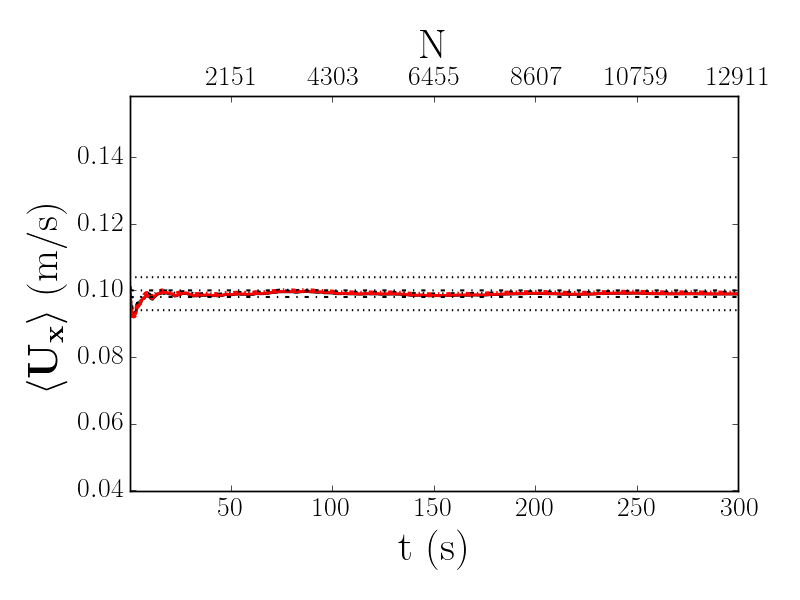
\includegraphics[width=7.5cm]{images/LDA_timeDependenceImages/4hz_x_400_z_40_MeanUx.png}\hfill
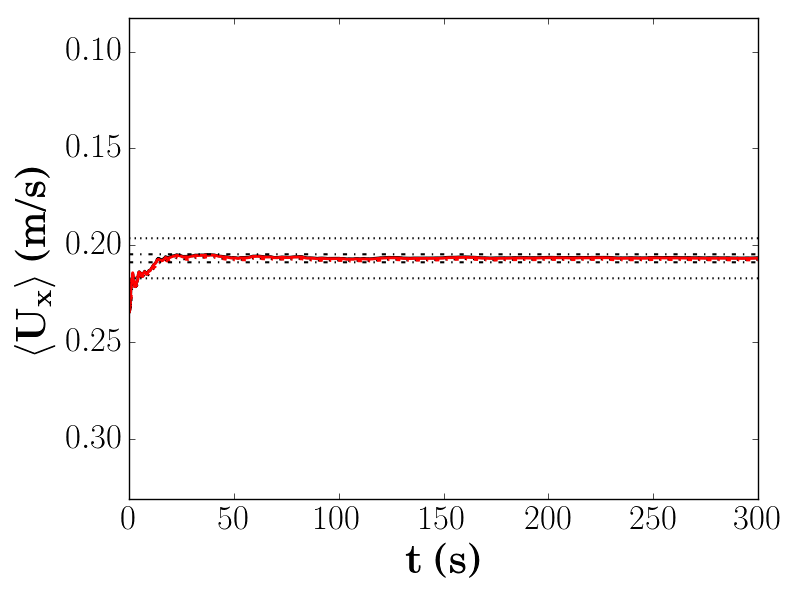
\includegraphics[width=7.5cm]{images/LDA_timeDependenceImages/8hz_x_400_z_40_MeanUx.png}\\
\caption{Mean streamwise velocity at $z$ locations \SI{1}{mm} (top), \SI{15}{mm} (middle) and \SI{40}{mm} (bottom) for pump speeds of \SI{4}{Hz} (images on the left) and \SI{8}{Hz} (images on the right). Dash-dotted lines represent unweighted data, solid lines represent weighted data. Black lines represent raw data, Red lines represent filtered data. $\pm 1\%$ and $\pm 5\%$ lines are represented by the feint dashed black lines.}
\label{figure:experiments:timeDependence:meanUx}
\end{figure}

\begin{figure}
\centering
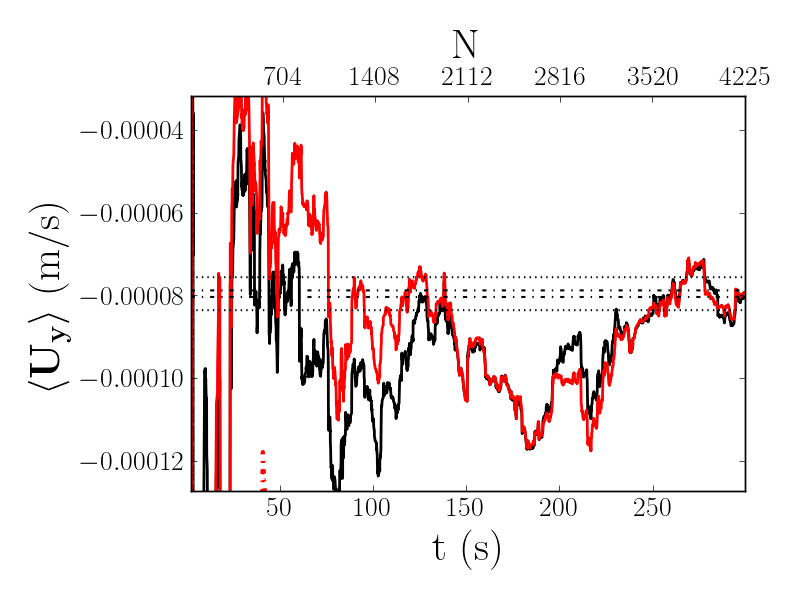
\includegraphics[width=7.5cm]{images/LDA_timeDependenceImages/4hz_x_400_z_1_MeanUy.png}\hfill
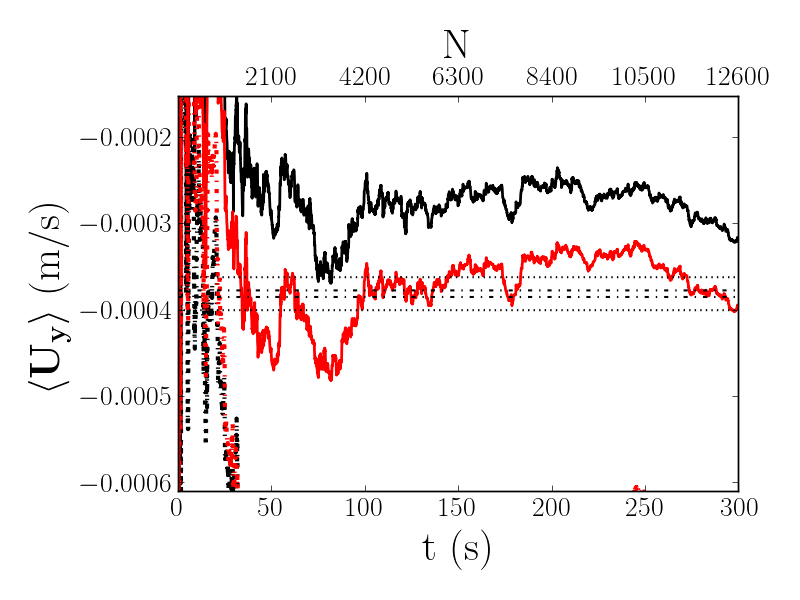
\includegraphics[width=7.5cm]{images/LDA_timeDependenceImages/8hz_x_400_z_1_MeanUy.png}\\
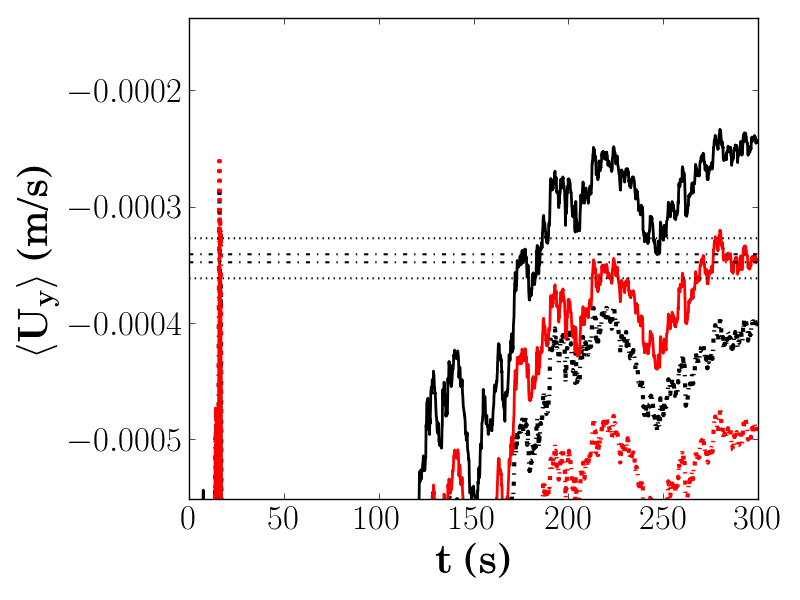
\includegraphics[width=7.5cm]{images/LDA_timeDependenceImages/4hz_x_400_z_15_MeanUy.png}\hfill
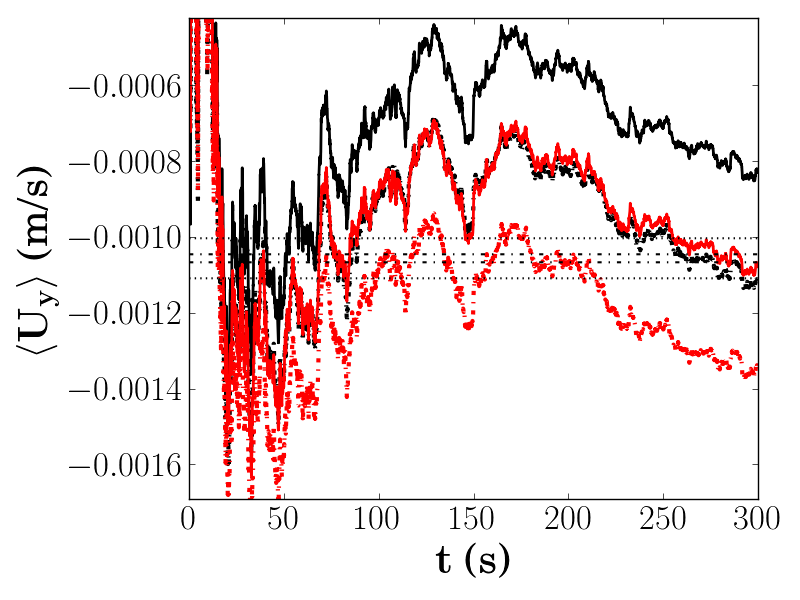
\includegraphics[width=7.5cm]{images/LDA_timeDependenceImages/8hz_x_400_z_15_MeanUy.png}\\
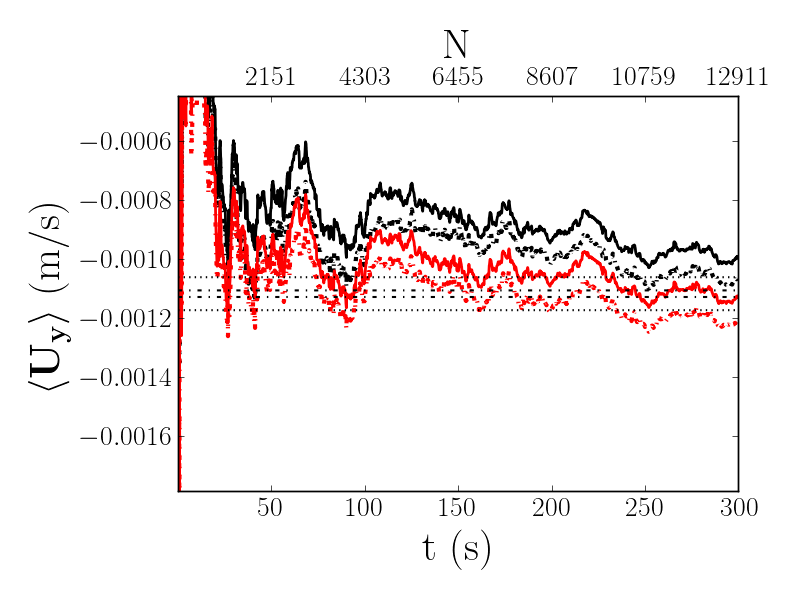
\includegraphics[width=7.5cm]{images/LDA_timeDependenceImages/4hz_x_400_z_40_MeanUy.png}\hfill
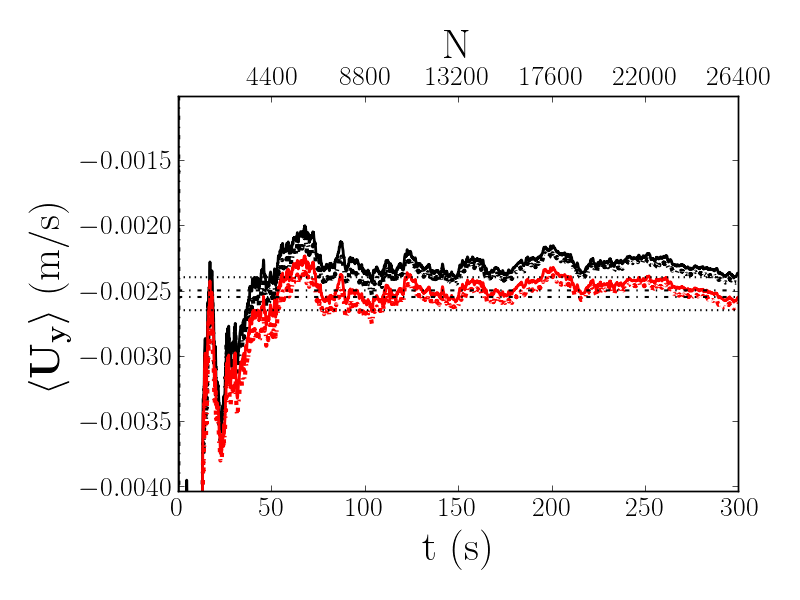
\includegraphics[width=7.5cm]{images/LDA_timeDependenceImages/8hz_x_400_z_40_MeanUy.png}\\
\caption{Mean wall-normal velocity at $z$ locations \SI{1}{mm} (top), \SI{15}{mm} (middle) and \SI{40}{mm} (bottom) for pump speeds of \SI{4}{Hz} (images on the left) and \SI{8}{Hz} (images on the right).}
\label{figure:experiments:timeDependence:meanUy}
\end{figure}

\begin{figure}
\centering
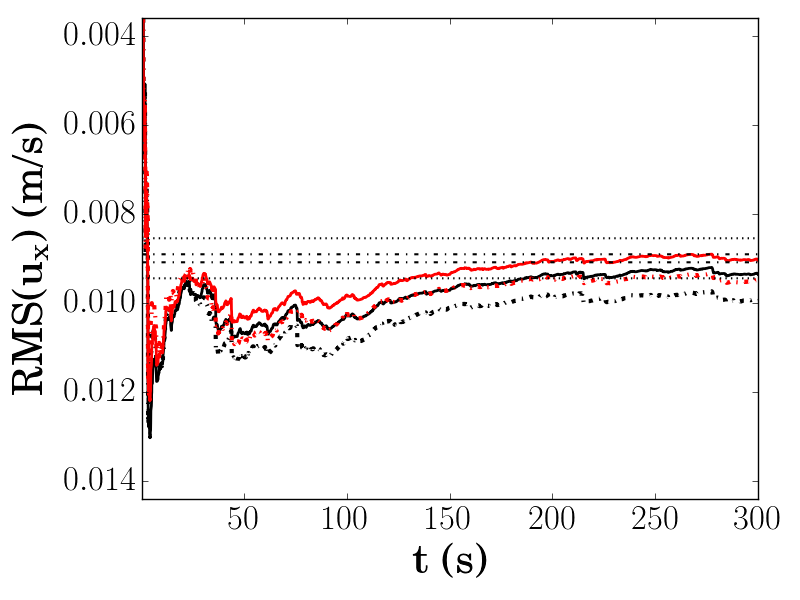
\includegraphics[width=7.5cm]{images/LDA_timeDependenceImages/4hz_x_400_z_1_RMSux.png}\hfill
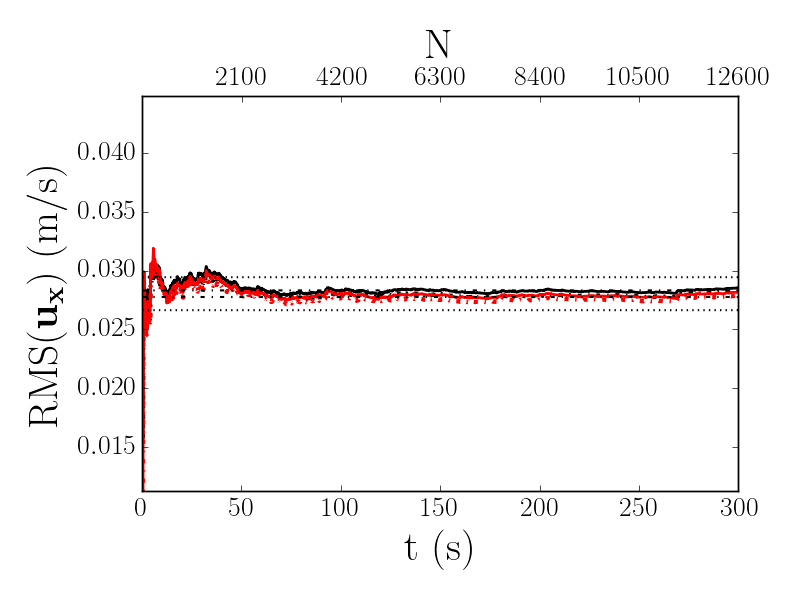
\includegraphics[width=7.5cm]{images/LDA_timeDependenceImages/8hz_x_400_z_1_RMSux.png}\\
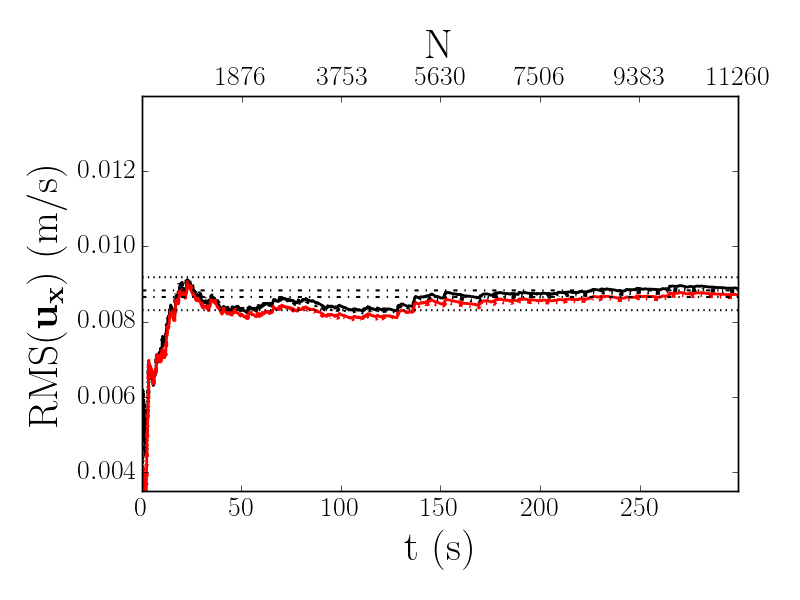
\includegraphics[width=7.5cm]{images/LDA_timeDependenceImages/4hz_x_400_z_15_RMSux.png}\hfill
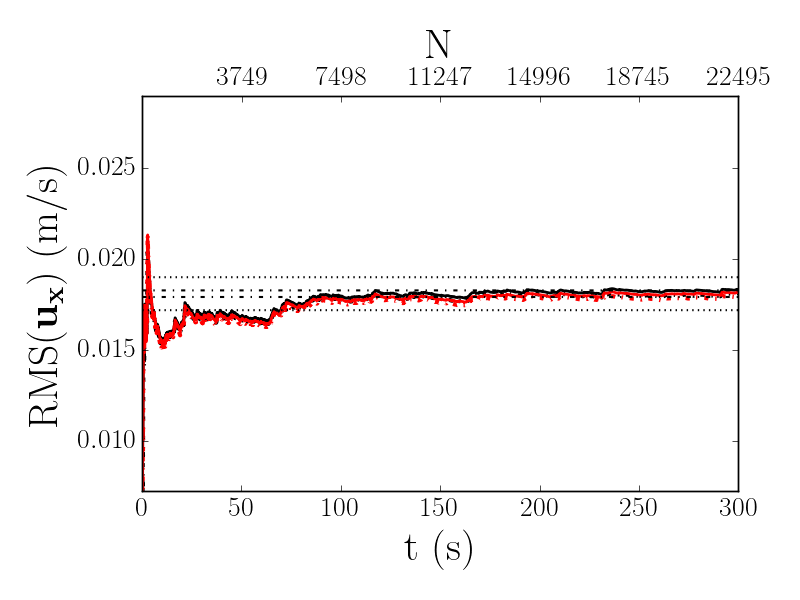
\includegraphics[width=7.5cm]{images/LDA_timeDependenceImages/8hz_x_400_z_15_RMSux.png}\\
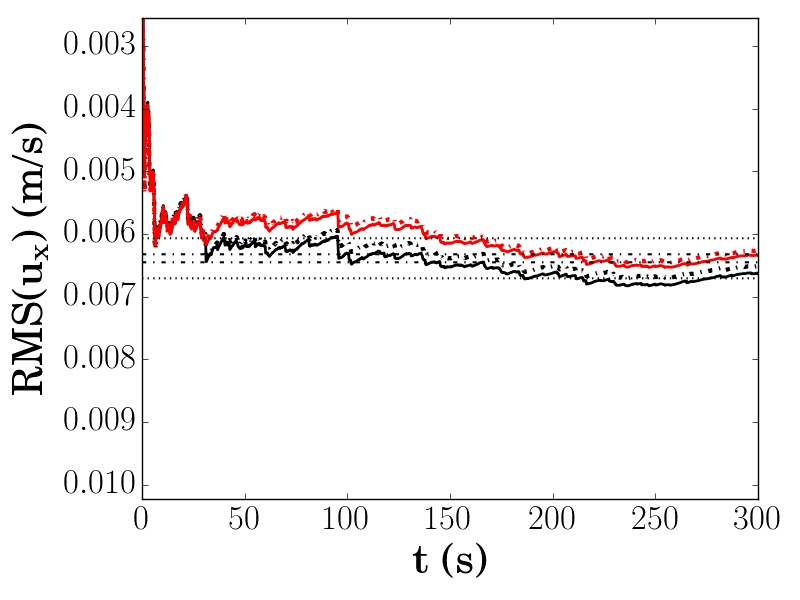
\includegraphics[width=7.5cm]{images/LDA_timeDependenceImages/4hz_x_400_z_40_RMSux.png}\hfill
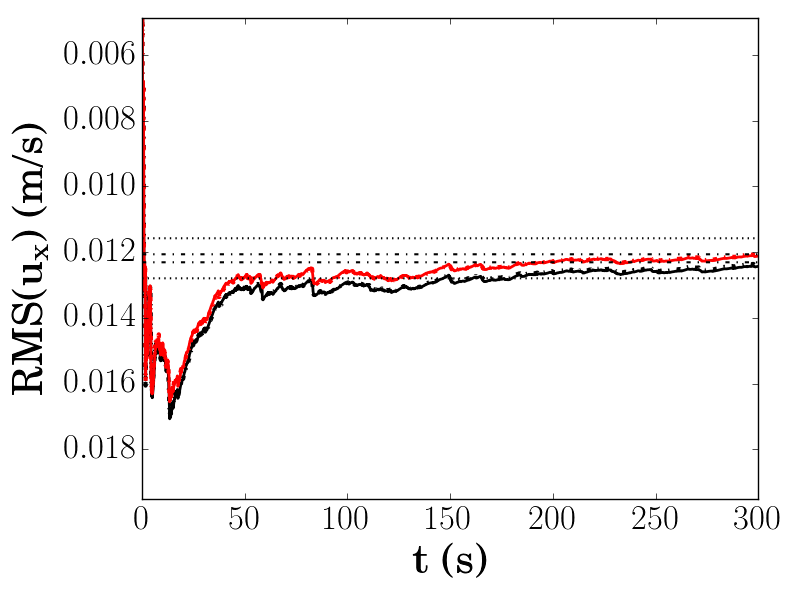
\includegraphics[width=7.5cm]{images/LDA_timeDependenceImages/8hz_x_400_z_40_RMSux.png}\\
\caption{RMS of the streamwise velocity fluctuations at $z$ locations \SI{1}{mm} (top), \SI{15}{mm} (middle) and \SI{40}{mm} (bottom) for pump speeds of \SI{4}{Hz} (images on the left) and \SI{8}{Hz} (images on the right).}
\label{figure:experiments:timeDependence:RMSux}
\end{figure}

\begin{figure}
\centering
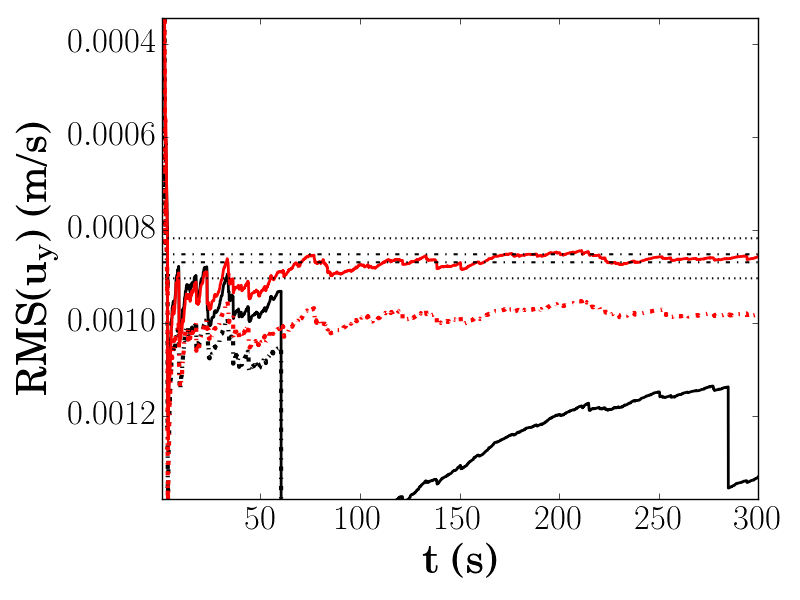
\includegraphics[width=7.5cm]{images/LDA_timeDependenceImages/4hz_x_400_z_1_RMSuy.png}\hfill
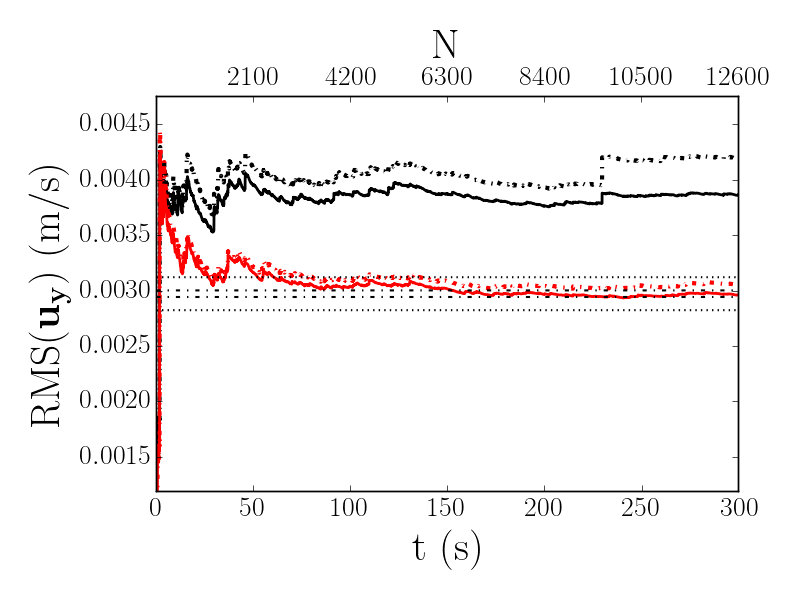
\includegraphics[width=7.5cm]{images/LDA_timeDependenceImages/8hz_x_400_z_1_RMSuy.png}\\
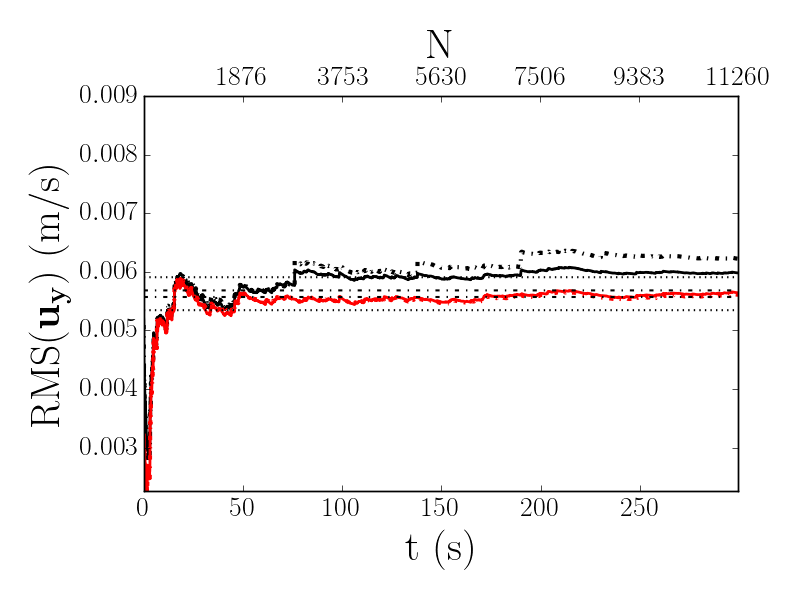
\includegraphics[width=7.5cm]{images/LDA_timeDependenceImages/4hz_x_400_z_15_RMSuy.png}\hfill
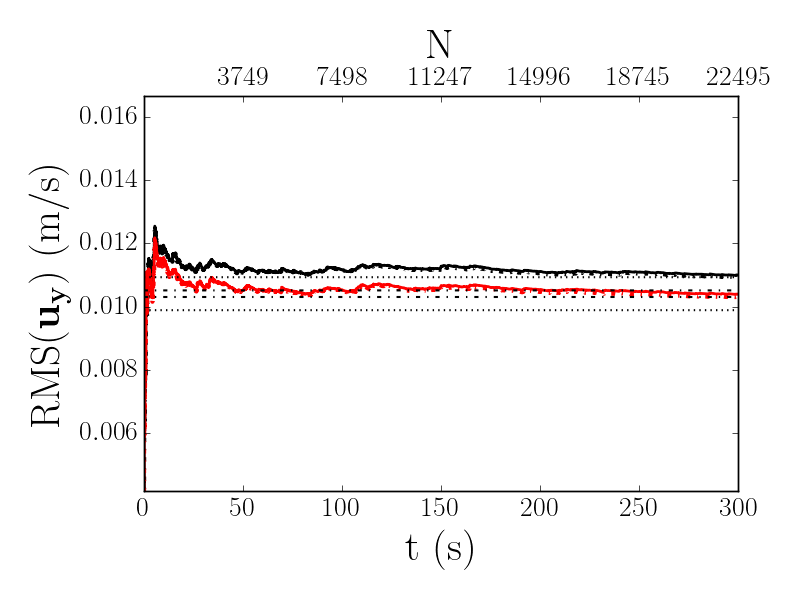
\includegraphics[width=7.5cm]{images/LDA_timeDependenceImages/8hz_x_400_z_15_RMSuy.png}\\
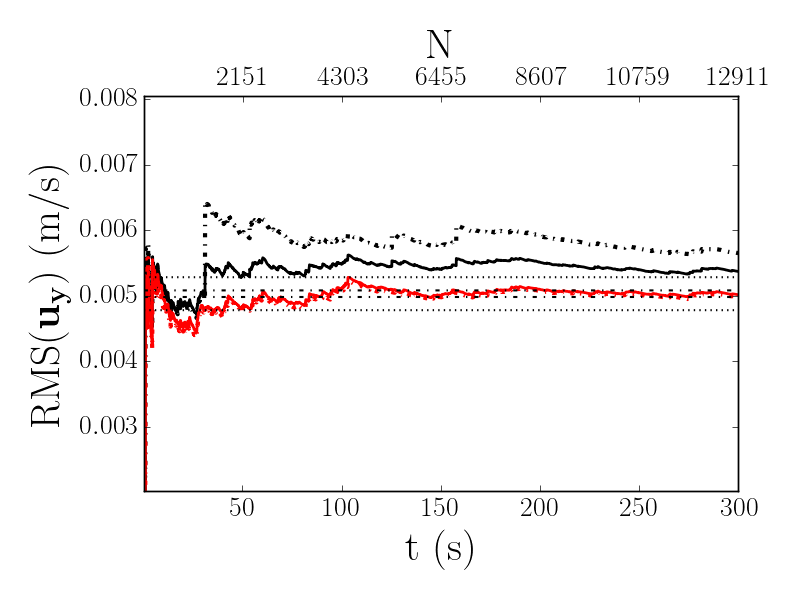
\includegraphics[width=7.5cm]{images/LDA_timeDependenceImages/4hz_x_400_z_40_RMSuy.png}\hfill
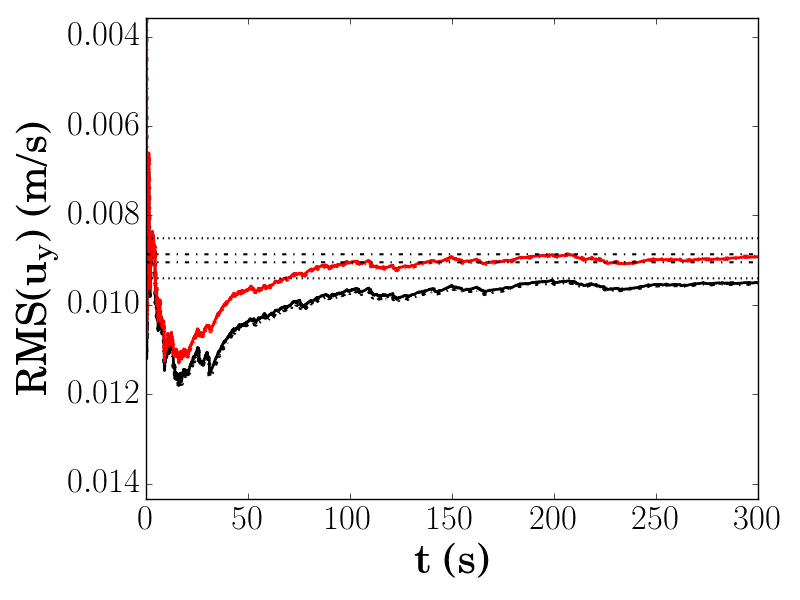
\includegraphics[width=7.5cm]{images/LDA_timeDependenceImages/8hz_x_400_z_40_RMSuy.png}\\
\caption{RMS of the wall-normal velocity fluctuations at $z$ locations \SI{1}{mm} (top), \SI{15}{mm} (middle) and \SI{40}{mm} (bottom) for pump speeds of \SI{4}{Hz} (images on the left) and \SI{8}{Hz} (images on the right).}
\label{figure:experiments:timeDependence:RMSuy}
\end{figure}

\begin{figure}
\centering
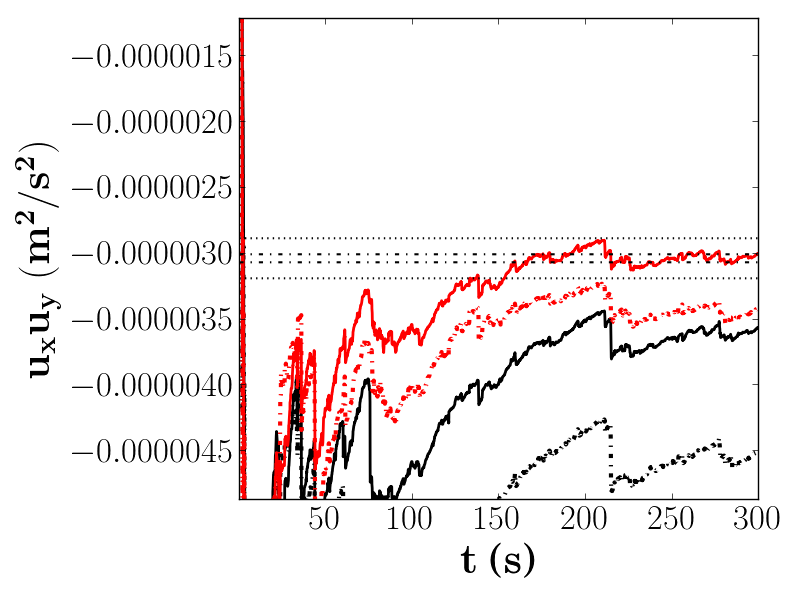
\includegraphics[width=7.5cm]{images/LDA_timeDependenceImages/4hz_x_400_z_1_uv.png}\hfill
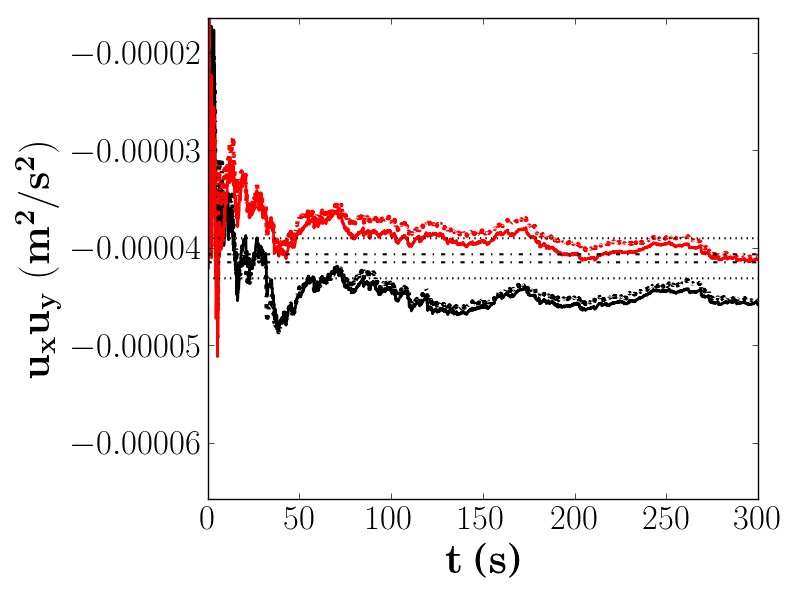
\includegraphics[width=7.5cm]{images/LDA_timeDependenceImages/8hz_x_400_z_1_uv.png}\\
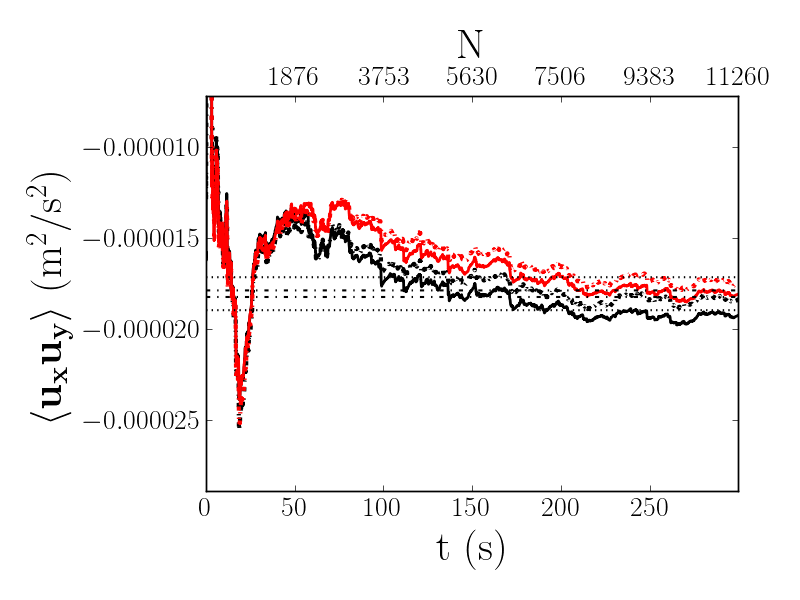
\includegraphics[width=7.5cm]{images/LDA_timeDependenceImages/4hz_x_400_z_15_uv.png}\hfill
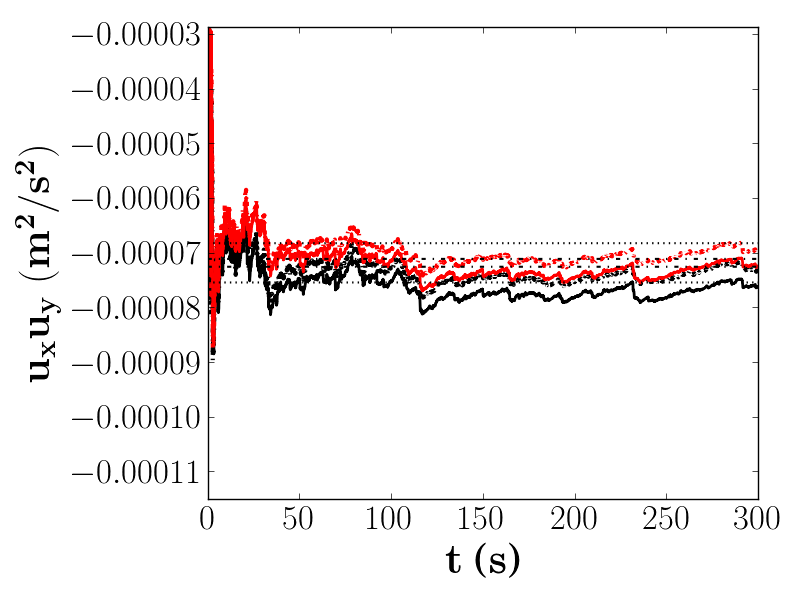
\includegraphics[width=7.5cm]{images/LDA_timeDependenceImages/8hz_x_400_z_15_uv.png}\\
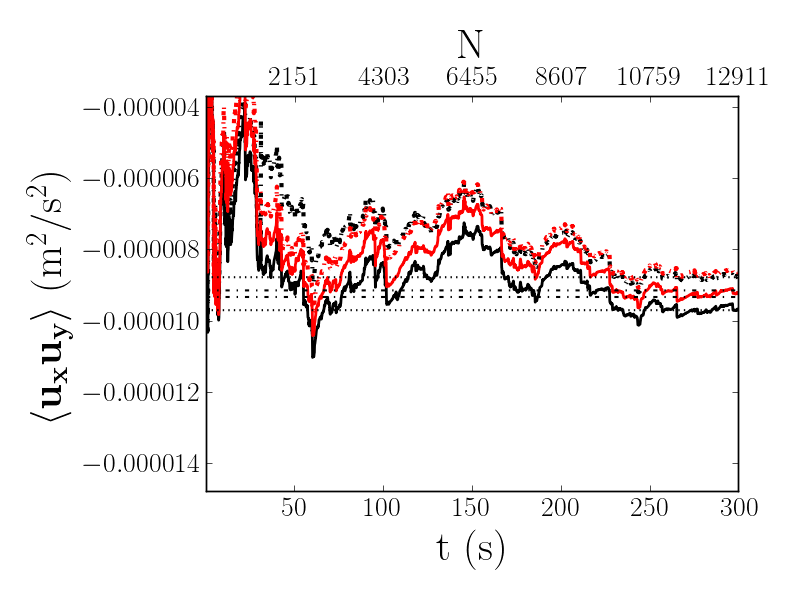
\includegraphics[width=7.5cm]{images/LDA_timeDependenceImages/4hz_x_400_z_40_uv.png}\hfill
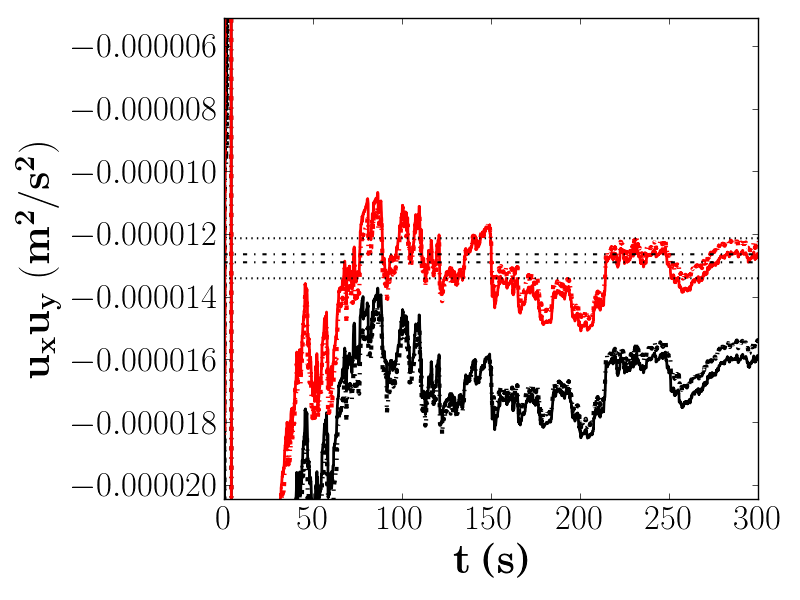
\includegraphics[width=7.5cm]{images/LDA_timeDependenceImages/8hz_x_400_z_40_uv.png}\\
\caption{Reynolds stresses, $u_x \text{u}_y$, at $z$ locations \SI{1}{mm} (top), \SI{15}{mm} (middle) and \SI{40}{mm} (bottom) for pump speeds of \SI{4}{Hz} (images on the left) and \SI{8}{Hz} (images on the right).}
\label{figure:experiments:timeDependence:uv}
\end{figure}
The purpose of these experiments is to both determine the amount of sampling time required for statistical quantities to converge, and estimate the error induced by sampling for less time. The quantities of interest are the mean streamwise ($\left<U_x\right>$) and wall-normal ($\left<U_y\right>$) velocities, the Root-Mean-Square (RMS) of the fluctuations of these velocity components (RMS($u_x$) and RMS($u_y$)), and the Reynolds stresses ($\left<u_x u_y \right>$). The mean and RMS quantities are evaluated by
\begin{equation}
\left<U_i\right> = \frac{1}{N}\sum^N_{j=1} U_{i,j}, \hspace{1cm}
\text{RMS}(u_i) = \sqrt{\frac{1}{N}\sum^N_{j=1} (u_{i,j})^2},
\end{equation}
where $u_i= U_i - \left<U_i\right>$ is the velocity fluctuation. The Reynolds stresses are calculated using
\begin{equation}
\left< u_x u_y \right> = \frac{1}{N}\sum^N_{j=1} (u_{x,j} u_{y,j}).
\end{equation}
%	NEED TO EXPLAIN HOW WE CALCULATE TIME DEPENDENCE!!
A compromise must be reached between spacial and temporal accuracy; if a long sampling time is required for convergence then the amount of time required to collect data increases, thus fewer points in space can be sampled in a given time period. The following data are gathered by sampling at three locations (\SI{1}{mm}, \SI{15}{mm} and \SI{40}{mm} from the flat plate) in the flow at two pump speeds (\SI{4}{Hz} and \SI{8}{Hz}). Several positions are chosen since the amount of sampling time required is dependent on the local velocity of the flow. It is therefore expected that close to the wall, statistics will require a longer averaging window. In order to assess convergence the statistics are estimated by averaging over the last 30 seconds of sampling time. $\pm 1\%$ and $\pm 5\%$ confidence intervals are estimated from this and plotted for each data set.

The impact of accounting for velocity bias and filtering poor data is also assessed through these experiments.
\\\\
Figure \ref{figure:experiments:filteringExample}:	This shows the phase space diagram for filtering poor data. 
\\
Figure \ref{figure:experiments:timeDependence:meanUx}: plots indicate several things:\\
1.	Weighting has a large effect near the wall but for z=15 and z=40 it has little impact\\
2.	filtering makes very little difference\\
3.	achieve convergence of 1\% at ~150s for both pump speeds near the wall. Get conv at 150s for slow speed and 60s at high speed for z=15mm. We get conv at ~30 sec for both flows far from the wall. \\
\\
Figure \ref{figure:experiments:timeDependence:meanUy}:\\
1.	Both weighting and filtering have a large impact on all of the plots\\
2.	we don't get convergence to 1\% for any data\\
3.	could be argued that we reach a 5\% convergence at 40mm for both data sets although little confidence of this without longer sampling times. \\
\\
Figure \ref{figure:experiments:timeDependence:RMSux}:\\
1.	filtering makes a difference close to wall\\
2.	weighting makes a difference for all\\
3.	conv is reached sooner for high speed flow than low speed for all distances\\
4.	interestingly the fast flow converges quicker close to the wall than far from it. (100 sec close to wall, 200 sec far from)\\
5.	low speed flow struggles to converge close to wall, possibly converges to 1\% at 250s but need more sampling time to confirm\\
6.	Generally takes longer to conv. than means.\\
\\
Figure \ref{figure:experiments:timeDependence:RMSuy}:\\
1.	Most notable change is the large spikes in the profiles which are removed when the filter is applied. These show up much more in RMS than means.\\
2.	Weighting makes much more difference for the slower speed than higher\\
3.	generally get quicker convergence for UyRMS than UxRMS, despite lack of convergence for UyMean.\\
4.	interestingly we get conv. close to wall before far from wall
\\\\
Figure \ref{figure:experiments:timeDependence:uv}:\\
1.	Same spikes are observed as in UyRMS BUT filtering doesn't remove them entirely!\\
2.	again, weighting makes a large difference for all data.\\
3.	Generally don't achieve convergence - need to sample for longer.\\
\\
Recommendations: sample for longer and for more points
-	Construct a polynomial for the estimated error for a given sampling time as a function of space.



\subsubsection{Streamwise Space Dependence}
Are we fully developed ..?\\
\begin{figure}
\centering
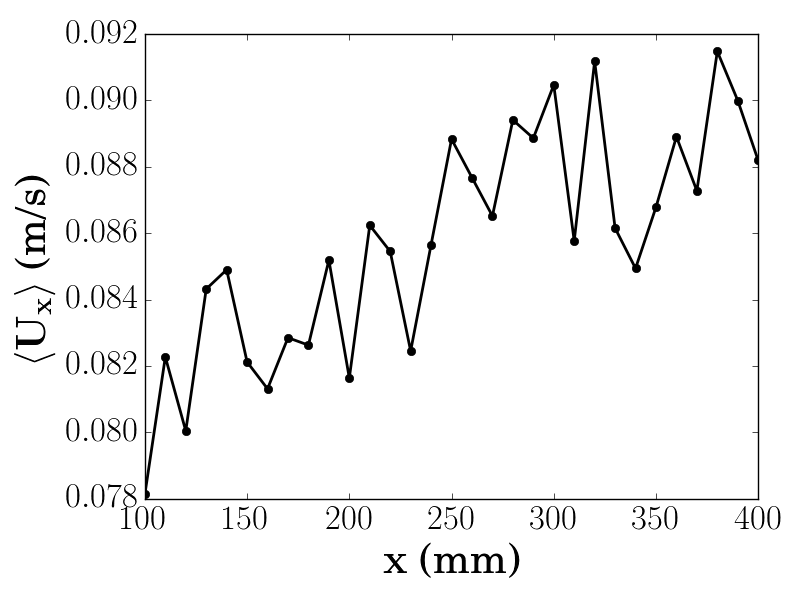
\includegraphics[width=7.5cm]{images/LDA_spaceDependenceImages/4Hz_15mm_MeanUx.png}\hfill
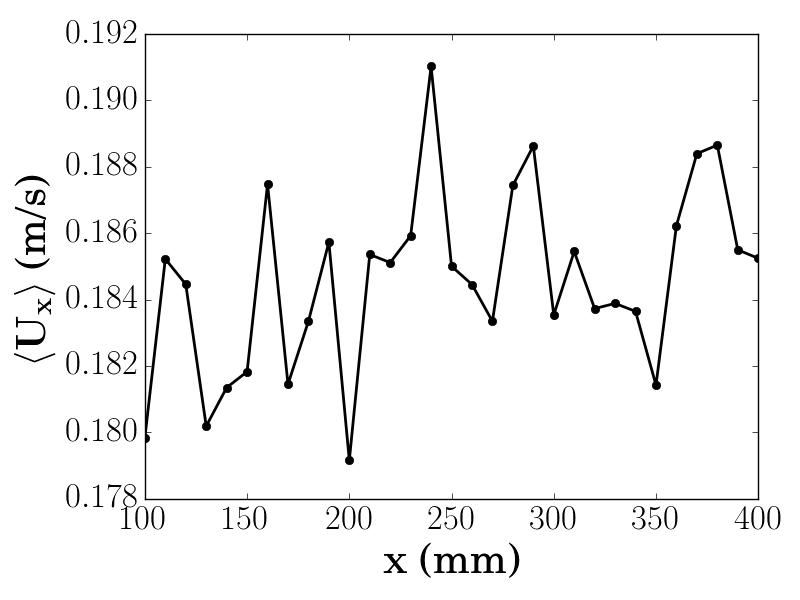
\includegraphics[width=7.5cm]{images/LDA_spaceDependenceImages/8Hz_15mm_MeanUx.png}\\
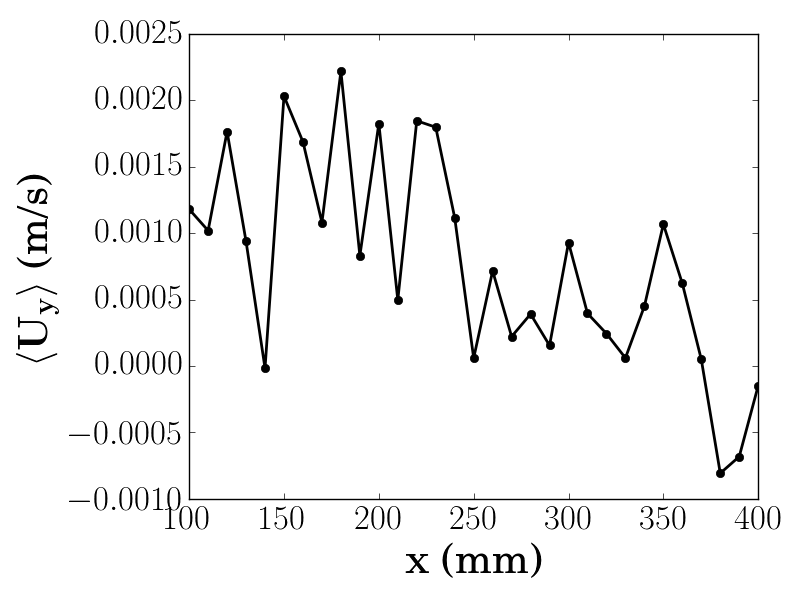
\includegraphics[width=7.5cm]{images/LDA_spaceDependenceImages/4Hz_15mm_MeanUy.png}\hfill
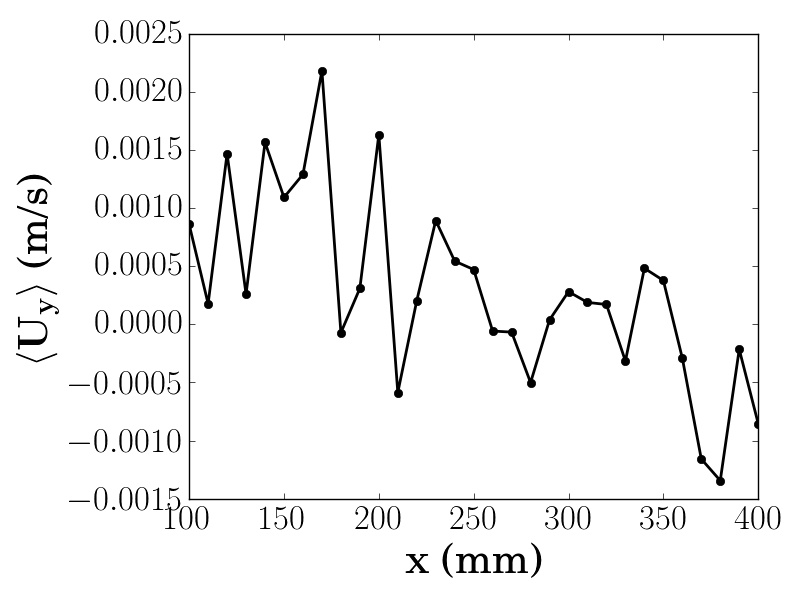
\includegraphics[width=7.5cm]{images/LDA_spaceDependenceImages/8Hz_15mm_MeanUy.png}\\
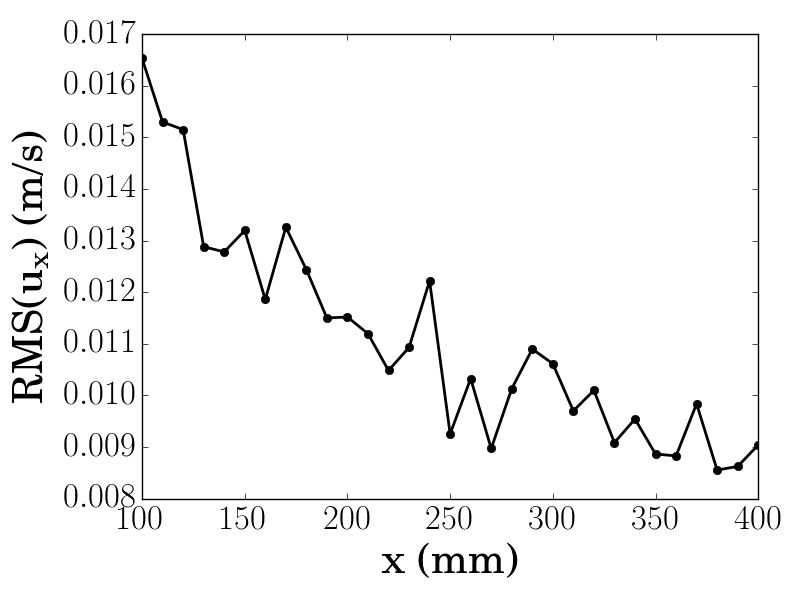
\includegraphics[width=7.5cm]{images/LDA_spaceDependenceImages/4Hz_15mm_RMSux.png}\hfill
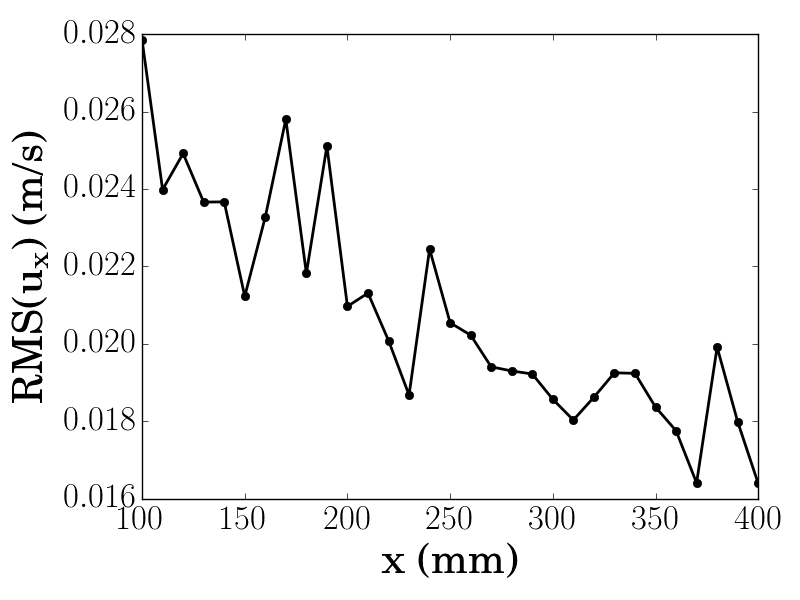
\includegraphics[width=7.5cm]{images/LDA_spaceDependenceImages/8Hz_15mm_RMSux.png}
\caption{Spatial dependence of statistical quantities at a location 15mm from the plate and pump speeds of \SI{4}{Hz} (left) and \SI{8}{Hz} (right).}
\label{figure:experiments:spaceDependence}
\end{figure}
%
\begin{figure}
\ContinuedFloat
\captionsetup{list=off,format=cont}
\centering
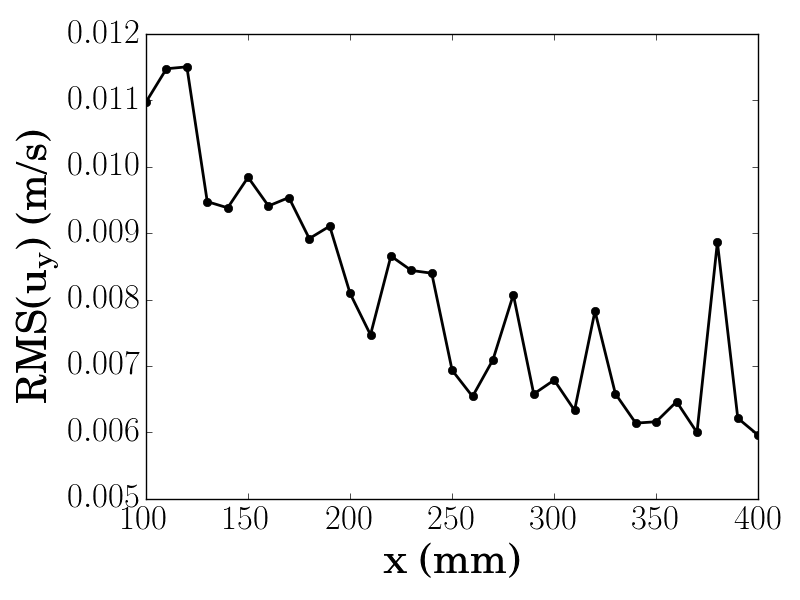
\includegraphics[width=7.5cm]{images/LDA_spaceDependenceImages/4Hz_15mm_RMSuy.png}\hfill
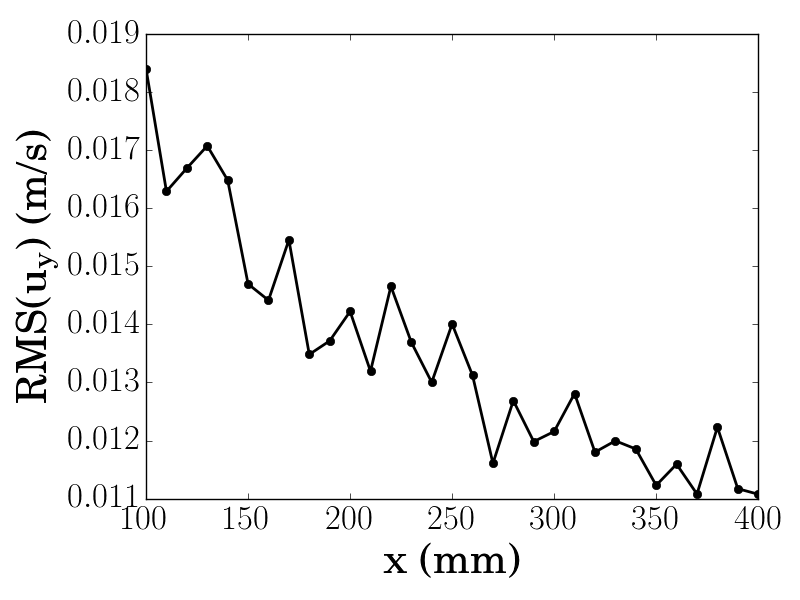
\includegraphics[width=7.5cm]{images/LDA_spaceDependenceImages/8Hz_15mm_RMSuy.png}\\
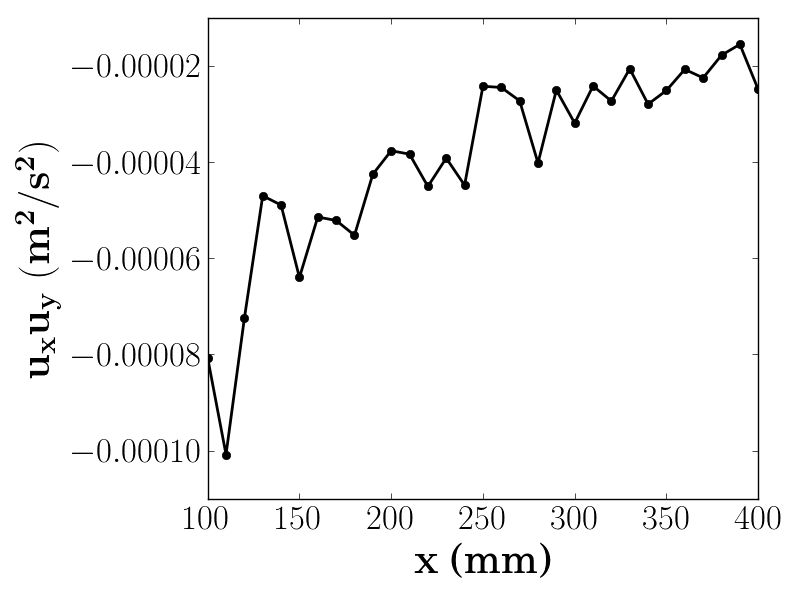
\includegraphics[width=7.5cm]{images/LDA_spaceDependenceImages/4Hz_15mm_uv.png}\hfill
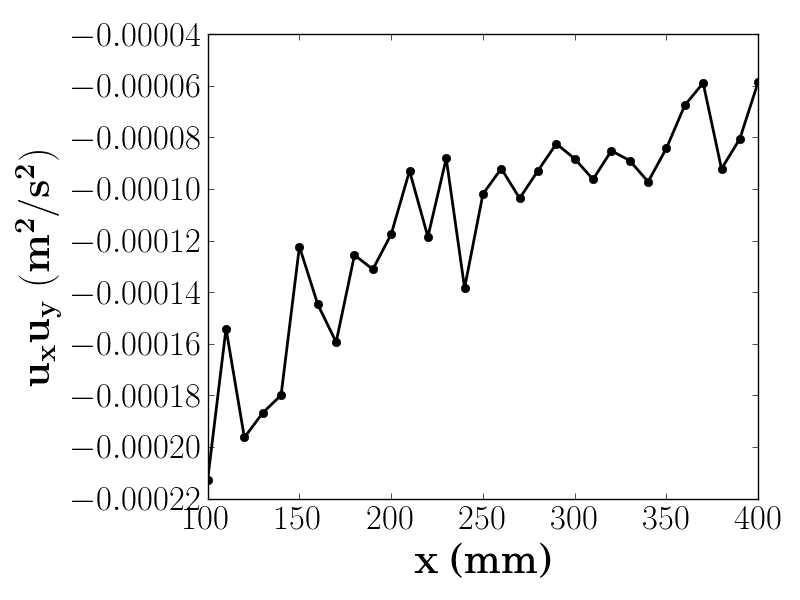
\includegraphics[width=7.5cm]{images/LDA_spaceDependenceImages/8Hz_15mm_uv.png}
\caption{For caption see Figure \ref{figure:experiments:spaceDependence}.}
\end{figure}
%

\subsubsection{Profile plot section}
\begin{figure}
\centering
\includegraphics[width=10cm]{images/LDA_profileImages/tempProfile.png}
\caption{Temporary velocity profile plot for a pump speed of 8Hz and a distance of 300mm.}
\end{figure}
Plot profiles of mean velocities, rms and Reynolds stresses. We can estimate how well we fit the law of the wall, Reynolds numbers and friction coefficients. 
\section{Work So Far ...}
A review of the literature indicates two areas that have not been adequately investigated: Analysis of the effect of scale geometry on the flow field, and the impact of scales on separating flows. Proprietary work has, so far, concentrated on the first of those areas, although the techniques adopted are transferable to the latter. A parametric study is to be carried out, in order to investigate the effects of scale geometry on the fluid flow. This tool will exploit the periodicities and symmetries associated with arrayed scales, resulting in an infinitely long and wide computational domain. For smooth walls, an extensive range of DNS data is available, making the validation of early work straight forward. The parametric tool requires several work packages to be completed before it can be used. In order to reduce computational expense, the parametric tool will adopt RANS methods. Experimental methods could be adopted to validate the RANS model, but these will only allow validation of the fields far from the scales, due to resolution issues. This will instead be combined with a high resolution LES, which will capture the flow around the scales. Progress has been made in three areas over the last 6 months:

\begin{itemize}
\itemsep0em
\item The creation of a simplified shark scale using CREO Parametric CAD software,

\item Preliminary experimentation with several meshing packages in order to select the most appropriate software,

\item and the implementation and validation of an LES channel flow.
\end{itemize}

Each of these will be discussed in the following sections.

\subsection{CAD: Replication of a shark scale}
\label{section:cad}
This Section details the process adopted to replicate and simplify a \textit{Poracanthodes sp.} fish scale (sampled by \cite{fletcher2014phd}) for fluid dynamic analysis. This particular scale was chosen due to its relatively simple geometry. Other sampled scales included other geometric features, such as riblets, which are not yet of interest. The implications of these additional features will be investigated through the parameter study. The Computer Aided Design (CAD) process, carried out using CREO Parametric software, is required in order to create an array of scales suitable for manufacture and LDA experimentation. The CAD model is also required in order to carry out numerical analysis; a body fitted mesh will be constructed using the CAD in order to adopt finite volume methods.

The scale sample, provided by \cite{fletcher2014phd}, is displayed in figure \ref{figure:scaleSample}. It can be observed from this image that there are many sharp edges that have been introduced, possibly by a lack of resolution from the scanning equipment, defects on the scale sample, or damage to the sample.
\begin{figure}[!b]
\centering
\includegraphics[width=6cm]{images/Scale_Replication_1.PNG}\hfill
\caption{\textit{Poracanthodes sp.} sample from \cite{fletcher2014phd}.}
\label{figure:scaleSample}
\end{figure}
There are also many asymmetries that exist, such as the wave-like shapes on the trailing edge of the scales. These features are likely due to the discrepancies between scale samples; even scales in tightly packed arrays are known to vary in geometry from scale to scale \citep{fletcher2014phd}. In addition to this, a large portion of the scale is embedded in the dermis of the fish and therefore has no effect on the hydrodynamics of the scale. For these reasons a simplified scale is created, based on the \textit{Poracanthodes sp.} sample. The simplified replica removes the sharp faceted features, the asymmetries and the portion of the scale that lies underneath the fish dermis.

\subsubsection{Methodology}
A coordinate system is fitted to the scale and 10 datum planes are created in the $xz$ plane with equal spacings between the first 7 and last 3 planes. The first set of planes extend to the point of maximum width of the sample and the last three are placed in order to capture the steep gradients beyond this point. A sketch is created at each of these planes resembling the cross section of the scale sample but using primitive shapes that can later be parametrised. An example of this is presented in Figure \ref{figure:crossSection};

the wave-like shapes on the downstream section of the scale has been removed and the sketch is symmetric about the central axis. This is achieved by using three arcs connected by tangential lines, reducing each section to three radius parameters, three vertical positions and a single horizontal position (as observed in Figure \ref{figure:crossSection}). Each sketch can therefore be represented by a displacement from the $y=0$ plane and 7 dimensions defining the sketch section. This makes parameter studies straight forward to implement in future work. 

\begin{figure}[!b]
\centering
\vcenteredhbox{\includegraphics[width=12cm]{images/cross_section_sketch.PNG}}
\caption{A comparison between a simplified cross section and the sampled scale cross section. The dimensions are scaled after the simplified scale is generated.}
\label{figure:crossSection}
\end{figure}

The sketches are blended together using a `protrusion blend' function, creating the CAD model on the right of Figure \ref{figure:blendedScale}. An undesirable feature of this technique is that the top surface is orthogonal to the defined datum plane. In order to create a more natural curved surface a warping tool, unique to Creo Parametric, is adopted. This tool creates a mesh around the object and allows free-hand manipulation of the surface by moving the mesh nodes. This process allows an organic Scale to be created which more closely resembles that of the original sample. However, parametrising the `warping' tool is non-trivial. Further work in this area will be carried out in order to develop a more systematic approach, but for initial experimentation this `one-off' scale is appropriate.

The final scale replica is compared against the scanned sample in Figure \ref{figure:scaleComparison}. The model is scaled to a height of $H^+ \sim 10$ at a Reynolds number of $Re_\tau = 180$ for preliminary meshing experiments. This will later be scaled to a suitable size for both 3D printing, LDA experiments and a high resolution LES. The scales are arranged into a staggered array (Figure \ref{figure:staggeredArray}) with an addition two parameters to define; a spacing in $x$ and in $z$. The exploitation of this periodic arrangement, through the use of CFD, will be discussed in Section \ref{section:meshing}.

\begin{figure}[!t]
\centering
\vcenteredhbox{\includegraphics[width=7.8cm]{images/Scale_Replication_3.PNG}}\hfill
\vcenteredhbox{\includegraphics[width=7.8cm]{images/Scale_Replication_9.PNG}}
\caption{Comparison of sampled scale (left) and simplified scale (right) with overlaying primitive cross sections displayed.}
\label{figure:blendedScale}
\end{figure}

\begin{figure}[!b]
\centering
\vcenteredhbox{\includegraphics[width=7cm]{images/Scale_Replication_10.PNG}}\hfill
\vcenteredhbox{\includegraphics[width=7.5cm]{images/Scale_Replication_11.PNG}}
\caption{Comparison of blended scale (left) and warped scale (right).}
\label{figure:warping}
\end{figure}

\begin{figure}[!t]
\centering
\vcenteredhbox{\includegraphics[width=7.5cm]{images/Scale_Replication_15.PNG}}\hfill
\vcenteredhbox{\includegraphics[width=7.5cm]{images/Scale_Replication_11.PNG}}
\\
\vspace{2cm}
\vcenteredhbox{\includegraphics[width=7.5cm]{images/Scale_Replication_16.PNG}}\hfill
\vcenteredhbox{\includegraphics[width=7.5cm]{images/Scale_Replication_12.PNG}}
\\
\vspace{2.5cm}
\vcenteredhbox{\includegraphics[width=7.5cm]{images/Scale_Replication_14.PNG}}\hfill
\vcenteredhbox{\includegraphics[width=7.5cm]{images/Scale_Replication_13.PNG}}
\caption{Comparison of sampled scale (left) and simplified scale (right).}
\label{figure:scaleComparison}
\end{figure}

\begin{figure}[!t]
\centering
\includegraphics[width=7.5cm]{images/array_progress_report.PNG}
\caption{Array of staggered scales for 3D printing.}
\label{figure:staggeredArray}
\end{figure}




\newpage
\subsection{Preliminary Meshing Experiments}
\label{section:meshing}
The meshing process is a large factor in optimising a parametric CFD study: being able to generate a high quality mesh without user interaction would cut simulation time significantly. In addition to this, the periodicity must be exploited by the CFD solver, thus periodic boundaries must be treated by the meshing software. An example of the periodic domain is displayed in Figure \ref{figure:periodicDomain}, meshed using STAR-CCM+. The scale array can be reconstructed by copying and translating the domain in the $z$ direction and mirroring the domain in the $x$ direction. Several other meshing packages have been investigated since September and assessed via the following criteria:

\begin{figure}[!b]
\centering
\includegraphics[width=12cm]{images/starccm_periodic_mesh.png}
\caption{Periodic mesh, created in STAR-CCM+, using the CAD scale documented in Section \ref{section:cad}. Periodicity exists between the $xz$ boundaries while symmetry planes are placed in the $yz$ planes.}
\label{figure:periodicDomain}
\end{figure}

\begin{itemize}
\itemsep0em
\item 
\textbf{Treatment of periodic boundaries}: Translational periodic boundaries can be applied by assuming the flow domain is infinitely long in the mean flow direction. Cell values are mapped between the two boundaries which requires their positions to be identical but translated downstream. When complex shapes, such as fish scales, intersect with these boundaries the meshing process becomes non-trivial. If the cell locations are identical then a `conformal' periodic boundary can be applied, otherwise `non-conformal' conditions are required. A non-conformal periodic boundary requires interpolation between faces, reducing the accuracy of the numerical scheme and introducing diffusive properties over the interface. 

\item 
\textbf{Cell types}: There are three common types of cells that are used for finite volume discretisation; hexahedral (6 faces), tetrahedral (4 faces), and polyhedral (arbitrary face count) \citep{durbin2007}. Hexahedral meshes are very common for simple geometric problems since it is straightforward to implement and maintain a high cell quality. However, fitting hexahedral cells to complex surfaces is non-trivial, making tetrahedral elements more suitable due to their flexibility, but with a compromise to numerical accuracy and convergence properties. In principle polyhedral cells can offer very smooth and high quality meshes, but they are generally more complex to create \citep{durbin2007}. Taking these into account, the desired meshing solver will contain polyhedral cells close to the fish scale surface, but blend into hexahedral cells, due to the simplicity of the rest of the channel domain. 

\item
\textbf{Scriptability}:
In order to reduce time, the meshing software used for the parameter study should be made scriptable to remove unnecessary user interaction. This would also allow small changes to be made to the CAD scale without requiring a new mesh case to be set up. This is less important for the LES model since only a single set of scales will be simulated.

\end{itemize}

Several software packages have been investigated, including both commercial and open source codes, which are summarised in Table \ref{table:meshSoftwareComparisons}. Advantages and disadvantages are present with each software, thus a compromise must be made when selecting a meshing package for both the LES case and the parametric study.

\begin{table}[!t]
\centering
\caption{Summary of tested meshing software in relation to the specified requirements of Section \ref{section:meshing}.}
\label{table:meshSoftwareComparisons}
\begin{tabular}{p{0.45\linewidth}p{0.45\linewidth}}
&\\
\textbf{ANSYS Fluent}	&	\\
\hline
\textbf{Pros}	&	\textbf{Cons}	\\
$\bullet$ High quality polyhedral cell mesh can be achieved,
&
$\bullet$ No blending between different cell types,
\\

$\bullet$ Mesher directly links to fluid solver,
&
$\bullet$ Conformal boundaries cannot be trivially set up.
\\

$\bullet$ Text based commands can be used and scripted, although this utility has not been investigated.
&
\\&\\	

\textbf{ANSYS ICEM CFD}	&	\\
\hline
\textbf{Pros}	&	\textbf{Cons}	\\
$\bullet$	High quality structured meshes can be achieved,
&
$\bullet$	Conformal boundaries cannot be trivially achieved,
\\
$\bullet$	Cell types can be blended (Hex. and Tet.),
&
$\bullet$	cannot create polyhedral cells.
\\
$\bullet$	Scriptable process.
&
\\&\\

\textbf{ANSYS Meshing}	&	\\
\hline
\textbf{Pros}	&	\textbf{Cons}	\\
$\bullet$ 	Scriptable through workbench,
&
$\bullet$	Little control over mesh quality,
\\
$\bullet$	can blend Hex. and Tet. cells.
&
$\bullet$	no polyhedral cells,
\\&\\

\textbf{STAR-CCM+}	&	\\
\hline
\textbf{Pros}	&	\textbf{Cons}	\\
$\bullet$ 	Primarily used for polyhedral meshing,
&
$\bullet$	Little control over quality and mesh refinement,
\\
$\bullet$	links to both inbuilt CAD for domain specification and CFD solver,
&
$\bullet$	No blending between different cell types.
\\
$\bullet$	Conformal boundaries are trivial to set up.
&
\\&\\

\textbf{SnappyHexMesh}	&	\\
\hline
\textbf{Pros}	&	\textbf{Cons}	\\
$\bullet$	Intuitive scriptability with effective link to OpenFOAM solver,
&
$\bullet$ Requires a lot of parameter tuning to generate an initial script,
\\
$\bullet$	full control over cell quality and refinement regions,
&
$\bullet$ requires a high quality .stl CAD file to generate a good quality mesh.
\\
$\bullet$	Primarily hexahedral cells but blends into polyhedral cells on complex surfaces.
&
$\bullet$	Complex features on periodic interfaces are non-conformal, but this can be blended into a conformal boundary further from this surface,

\end{tabular}
\end{table}

Both STAR-CCM+ and SnappyHexMesh have significant advantages over the other tested packages; STAR-CCM+ allows the generation of a smooth polyhedral mesh with conformal boundaries but requires more user interaction to ensure the mesh quality is appropriate. SnappyHexMesh is naturally scriptable and enforces specified quality criteria. However, a mix of conformal and non-conformal boundary conditions are required for the algorithm to work properly. For this reason, the high resolution LES model will be implemented using a polyhedral mesh, specified in STAR-CCM+. The parameter study will be carried out using SnappyHexMesh. Both sets of simulations will be carried out using the OpenFOAM fluid solver.

In terms of mesh generation, work over the following 6 months will consist of performing LES on a polyhedral mesh, in order to determine appropriate solver and discretisation settings to achieve comparable results to those presented in Section \ref{section:les}. In addition to this, appropriate mesh parameters will be determined for the SnappyHexMesh case and RANS simulations will be carried out on this domain to assess mesh independence and the influence of RANS model choice on the solution. This information will be used to create an appropriate sizing for the LES mesh.

\subsection{Application of Reynolds-Averaged Navier-Stokes to a periodic shark scale domain}
\label{section:rans}
Dependency analysis of RANS methods on a periodic shark scale domain.
Dependencies include MI, DI, model I, Numerics I, Tol I ...
The results will form the basis for the mesh resolution for the LES and the RANS studies. Before carrying out further RANS the results will be validated against a LES. 

\subsubsection{Problem definition}
As discussed? The Reynolds equations are given by

\begin{equation}
\frac{\overline{D} \langle U_i \rangle }{ \overline{D} t}
=
-\pdev{\langle P \rangle}{x_i}
+
\nu
	\left(
	\pdev{\langle U_j \rangle}{x_i}
	+
	\pdev{\langle U_i \rangle}{x_j} 
	\right)
+
\pdev{\langle u_i u_j\rangle}{x_i}.
\end{equation}
and the continuity equation by

\begin{equation}
\pdev{\langle U_i\rangle}{x_i}=0,
\end{equation}
where $\langle \phi \rangle$ represents the ensemble average of $\phi$. The present work adopts the turbulent viscosity hypothesis whereby the Reynolds stresses are estimated using

\begin{equation}
\left< u_i u_j \right> = \frac{2}{3}k \delta_{ij} - \nu_T \left( 
	\pdev{\left< U_i \right>}{x_j} + \pdev{\left< U_j \right>}{x_i}	\right).
\end{equation}

In order to model $\nu_T$ the model of (REF) is adopted, whereby transport equations for $k$, the turbulent kinetic energy, and $\omega$, the ...? are solved. 


These equations are similar in appearance as the Navier-Stokes equations \eqref{equation:fundamentalEquations:momentum} but require information about the Reynolds stresses, $\langle u_i u_j \rangle$. This forms the basis of the RANS ideology, whereby \eqref{equation:fundamentalEquations:meanContinuity} and \eqref{equation:fundamentalEquations:ReynoldsEquations} are solved for $\langle U_i \rangle$ and $\langle P \rangle$ by modelling the Reynolds stresses. There have been many proposed models to close this system of equations with varying accuracy and expense. A widely adopted approach to modelling these stresses is the turbulent-viscosity hypothesis which assumes
\begin{equation}
\left< u_i u_j \right> = \frac{2}{3}k \delta_{ij} - \nu_T \left( 
	\pdev{\left< U_i \right>}{x_j} + \pdev{\left< U_j \right>}{x_i}	\right),
\end{equation}
where $\nu_T(\boldsymbol{x},t)$ is the turbulent viscosity, analogous to the molecular viscosity. Algebraic relationships for $\nu_T$ have been suggested, such that $\nu_T=l_m^2 \left| (\partial \left<U\right> / \partial y   \right|$, but these are reliant on the specification of the mixing length $l_m$. 

\begin{equation}
\nu_T = c k^{1/2} l_m = C_\mu k^2/\epsilon,
\end{equation}


\begin{equation}
\pdev{k}{t} + \left< U_i \right> \cdot \nabla k = -\nabla \cdot T_i' + \mathcal{P} - \epsilon 
\end{equation}

\begin{equation}
T_i' = \frac{1}{2} \left< u_i u_j u_j \right> + \left< u_i P' \right> - 2 \nu \left< u_j s_{ij} \right>.
\end{equation}
where $P'$ is the fluctuation component of the kinematic pressure. Further assumptions: the flux, $T_i'$ is modelled using gradient diffusion, i.e 
\begin{equation}
T_i' = -\frac{\nu_T}{\sigma_{k}} \nabla k,
\end{equation}
where the turbulent Prandtl number is generally taken as $\sigma_k=1$. This physically asserts that due to velocity and pressure fluctuations there is a flux of k down the gradient of k \citep{pope2001}.

The equation for omega is entirely empirical:
\begin{equation}
\pdev{\omega}{t}  + \left< U_i \right> \cdot \nabla \omega = \nabla \cdot \left( \frac{\nu_T}{\sigma_{\omega}} \nabla \omega \right) + C_{\omega 1} \frac{\mathcal{P} \omega}{k} - C_{\omega 2} \omega^2
\end{equation}
By taking $\omega \equiv \epsilon /k$ and substituting into $\epsilon$ equation we get
\begin{equation}
\pdev{\omega}{t}  + \left< U_i \right> \cdot \nabla \omega = \nabla \cdot \left( \frac{\nu_T}{\sigma_{\epsilon}} \nabla \omega \right) + (C_{\varepsilon 1}-1) \frac{\mathcal{P} \omega}{k} - (C_{\varepsilon 2}-1) \omega^2 + \frac{2 \nu_T}{\sigma_\epsilon k}\nabla \omega \cdot \nabla k
\end{equation}


-present k and epsilon equations
-indicate what each term is - including the weighting factor
-Then introduce the FV method and how equations are discretised over our domain - BC. 




\subsubsection{Results and discussion}

Introduction: - what are we doing, why, how ..
dependency studies
-MI, DI, models, tolerances, disc. schemes etc. 
-Eventually validate against LES 
-Then we can start varying parameters to see effects on the flow field
Methodology: - meshing parameters and models used
- show domain and BCs,
-numerical methods,
Results: - MI results for contour plots over surface, profile plots in wall-normal direction.



\subsection{Large eddy simulation of a channel flow}
\label{section:les}
In order to exploit periodicity, an infinitely long and wide channel flow with scales on one wall will be simulated. Large-eddy simulation will be adopted in order to model the flow at a feasibly high resolution for a bulk Reynolds number greater than $Re_b = 20\ 000$. The precise Reynolds number will be determined later this year when designing the LDA experiments. Before implementing the LES on a channel flow with scales, the code is validated with smooth walls. This is carried out at a low Reynolds number of $Re_\tau = 180$ to make use of the extensive DNS database of \cite{vreman2014}. By validating at this Reynolds number we can determine suitable model and solver parameters without requiring extensive computing costs. Over the following year the model will be extended to a high Reynolds number to provide a base case for both comparisons against fish scale surfaces, and an estimation of the number of cells required.

\subsubsection{Mathematical Model}
\label{section:mathematicalModel}
Large eddy simulation is a technique used to study turbulence whereby the large turbulent structures are resolved and the small structures are modelled as a stress term. This is achieved by decomposing the velocity field into a filtered and residual term so that $\vecti{U} = \overline{\vecti{U}} + \vecti{u}'$. The filtered momentum (\ref{equation:momentum}) and continuity (\ref{equation:continuity}) equations \citep{pope2001} are defined as
\begin{equation}
\label{equation:momentum}
\pdev{\vecti{\overline{U}}}{t} + \pdev{\vecti{\overline{U}} \vectj{\overline{U}}}{\vectj{x}} - \pdev{}{\vectj{x}}(\matij{\overline{\sigma}} + \matij{\tau}) = - \pdev{\overline{P}}{\vecti{x}},
\end{equation}
and
\begin{equation}
\label{equation:continuity}
\pdev{\vecti{\overline{U}}}{\vecti{x}} = 0,
\end{equation}
where $\matij{\overline{\sigma}} = 2\nu \matij{\overline{S}}$ represents the resolved viscous stress tensor, $\overline{P} = \overline{p}/\rho$ is the resolved kinematic pressure, and $\matij{\overline{S}} = \frac{1}{2}\left( \pdev{\vecti{\overline{U}}}{\vectj{x}} + \pdev{\vectj{\overline{U}}}{\vecti{x}} \right)$ is the filtered rate of strain tensor. $\tau_{ij} = \vecti{\overline{U}} \vectj{\overline{U}} - \overline{\vecti{U} \vectj{U}}$ represents the effect of the unfiltered velocity field on the filtered field. This may be approximated using the model of \cite{smagorinsky1963}:
\begin{equation}
\label{equation:tau}
\matij{\tau}-\frac{1}{3}\matij{\delta}\tau_{kk} = 2\nu_{t} \matij{\overline{S}},
\end{equation}
where $\nu_t$ is the sub-grid scale viscosity. \cite{smagorinsky1963} defines this sub-grid scale viscosity as
\begin{equation}
\label{equation:smagorinsky}
\nu_t = (C_s \Delta)^2 |\overline{S}|,
\end{equation}
where $C_s$ is the Smagorinsky constant and $\Delta$ is the filter width, based on the local grid size. The magnitude of the filtered rate of strain tensor is defined as $|\overline{S}|= (2 \matij{\overline{S}} \matij{\overline{S}})^{1/2}$. The Smagorinsky model assumes a constant value of $C_s = 0.17$ \citep{smagorinsky1963}. However, the assumption that $C_s$ does not vary in space or time is a strong limitation to the model, as will be further discussed in section \ref{section:lesResults}. An alternative method, first suggested by \cite{germano1991}, estimates the coefficient by filtering \eqref{equation:momentum} and \eqref{equation:continuity} a second time. By applying this filter we can define an addition stress term, equivalent to (\ref{equation:tau}) just on a coarser grid of filter width $\widetilde{\Delta} = 2\Delta$: $\matij{T}-\frac{1}{3}\matij{\delta}T_{kk} =\vecti{\widetilde{\overline{U}}}\vectj{\widetilde{\overline{U}}}-\widetilde{\overline{\vecti{U}\vectj{U}}}$. By adopting the Germano identity \citep{germano1991}, we relate the scales of motion between the two filter widths:
\begin{equation}
\label{equation:germano}
\matij{L} = \matij{T}^r - \matij{\widetilde{\tau}}^r = \vecti{\widetilde{\overline{U}}}\vectj{\widetilde{\overline{U}}} - \widetilde{\vecti{\overline{U}}\vectj{\overline{U}}}.
\end{equation}
Unlike the equations for $\tau_{ij}$ and $T_{ij}$, equation \ref{equation:germano} can be solved from the filtered velocity field.  Assuming $\matij{T}$ takes the same form as $\matij{\tau}$, $L_{ij}$ can be solved to find $C_s$:
\begin{equation}
L_{ij} = 2\Delta^2 \left[	\widetilde{C_s^2 |\overline{S} | \matij{\overline{S}}} - 4 C_s^2 |\widetilde{\overline{S}}| \matij{\widetilde{\overline{S}}}		 \right].
\end{equation}
This represents 5 equations with 1 unknown, the error of which is given by
\begin{equation}
\label{equation:CsError}
e_{ij} = 	L_{ij} - M_{ij}C_s^2			,
\end{equation}
where $$M_{ij} =  2\Delta^2 \left[	\widetilde{|\overline{S} | \matij{\overline{S}}} - 4 |\widetilde{\overline{S}}| \matij{\widetilde{\overline{S}}} \right].$$
It is assumed that the constant $C_s$ does not vary spatially between the scales $\Delta$ and $2\Delta$, allowing it to be taken out of the filter term.

Typically the error is minimised by differentiating equation (\ref{equation:CsError}) with respect to $C_s^2$. However, this method requires both spatial averaging, in homogeneous directions, and clipping, in order to ensure $C_s$ remains positive (energy dissipating). An alternative to this restrictive dynamic model is to average along particle paths using the model of \cite{meneveau1996}. In a Lagrangian frame of reference, the trajectory of a fluid particle for earlier times $t'<t$ is given by
\begin{equation}
\label{equation:particlePath}
\vect{z}(t') = \vect{x} - \int_{t'}^t \overline{\vect{u}}(\vect{z}(t''),t'')dt''.
\end{equation}
In terms of the Lagrangian description the error to be minimised, (\ref{equation:CsError}), is
\begin{equation}
\label{equation:lagrangianCsError}
e_{ij}(\vect{z},t') = 	L_{ij}(\vect{z},t') - M_{ij}(\vect{z},t')C_s^2(\vect{x},t'),
\end{equation}
where it is assumed that $C_s$ can be removed from the filter by assuming it does not vary strongly over the scale of the test filter, an assumption that is investigated and justified by \cite{meneveau1996}. In order to minimise this error we define the total error as the pathline accumulation of the local error squared, 
\begin{equation}
\label{equation:ErrorSquared}
E = \int_{-\infty}^t e_{ij}(\textbf{z}(t'),t')e_{ij}(\textbf{z}(t'),t') W(t-t') dt',
\end{equation}
where $W(t-t')$ is a weighting function, introduced in order to control the contributions from times closer to $t$. Differentiating with respect to $C_s^2$, and making use of (\ref{equation:lagrangianCsError}), we obtain
\begin{equation}
\label{equation:CsFlmFmm}
C_s^2(\vect{x},t) = \frac{f_{LM}}{f_{MM}},
\end{equation}
where
\begin{equation}
\label{equation:flm}
f_{LM} = \int_{-\infty}^t L_{ij}M_{ij}(\vect{z}(t'),t') W(t-t') dt',
\end{equation}
and
\begin{equation}
\label{equation:fmm}
f_{MM} = \int_{-\infty}^t M_{ij}M_{ij}(\vect{z}(t'),t') W(t-t') dt'.
\end{equation}
A convenient choice of the weighting function is $W(t-t')=T^{-1} e^{-(t-t')/T}$ \citep{meneveau1996}. This results in two transport equations for $f_{LM}$ and $f_{MM}$ rather than backward integrals in time:
\begin{equation}
\label{equation:flmTransport}
\frac{D f_{LM}}{Dt} = \frac{1}{T}(L_{ij}M_{ij} - f_{LM}),
\end{equation}
\begin{equation}
\label{equation:fmmTransport}
\frac{D f_{MM}}{Dt} = \frac{1}{T}(M_{ij}M_{ij} - f_{MM}).
\end{equation}
$T$ represents a timescale that controls the memory length. There are some natural choices for this parameter, highlighted by \cite{meneveau1996}, whereby the timescale can be controlled by the values of $f_{LM}$ and $f_{MM}$. By taking $T=\theta \Delta (f_{LM} f_{MM})^{-1/8}$, where $\theta$ is a constant of order unity, the memory time will be reduced in both regions of high straining (high $f_{MM}$) and large nonlinear energy transfer (high $f_{LM}$). Typically $\theta=1.5$ for most cases, although there is some solution dependence on this value. This dependency will be investigated in future work. 

With these parameters now defined, the transport equations (\ref{equation:flmTransport}) and (\ref{equation:fmmTransport}) can be solved and used to determine $C_s$. The turbulent stress tensor equation, (\ref{equation:tau}), can now be solved, closing our set of equations.

\subsubsection{Numerical Implementation}
The equations are solved using OpenFOAM, a finite volume platform. The equations are discretised over a channel of dimensions $4.2\delta \times 2\delta \times 12.6\delta$ where $\delta$ is the channel half height. Similar dimensions are used by several authors such as \cite{moser1999}, and \cite{vreman2014} for a Reynolds number of $Re_\tau = 180$, although the influence of domain size on the turbulent statistics is still poorly understood \citep{vreman2014}. Three simulations are presented in this report, one which which solves equations for only half the channel height and applies symmetry boundary conditions at the central plane, $y=\delta$. If validated, this model could reduce the number of required cells. The half channel simulation adopts a constant value of $C_s = 0.17$, validated against a full channel simulation using the same model. The final simulation adopts the dynamic Lagrangian model discussed in Section \ref{section:mathematicalModel}.

The mesh statistics are presented in Table \ref{table:meshStatistics}. The total number of cells is $\sim 4M$, much fewer than an equivalent finite difference DNS of \cite{vreman2014} who used $\sim 33M$ grid points. A Cosine distribution is adopted in the wall-normal direction in order to capture the large gradients close to the wall. The y-normal boundary conditions can be observed from Table \ref{table:boundaryConditions}. The boundary conditions for $f_{LM}$ and $f_{MM}$ are defined by \cite{meneveau1996}. Periodic boundary conditions are applied in both streamwise and spanwise direction with a forcing term added to the momentum equation (\ref{equation:momentum}) in order to maintain a constant bulk Reynolds number in the $z$ direction. The forcing term is derived by decomposing the pressure gradient into an average and fluctuating component; the average pressure gradient is adjusted each timestep in order to ensure a fixed mean velocity through the periodic faces, $ \overline{\vect{U}}_{ave} $. A description of this technique is presented by \cite{murthy1997}.

\begin{table}[!b]
\centering
\caption{Mesh statistics for the three LES cases. The half channel case takes $N_y = 64$}
\label{table:meshStatistics}
\begin{tabular}{|l|l|l|l|l|l|l|}
\hline
$N_x$  & $N_y$  & $N_z$  & $\Delta x^+$ & $\Delta z^+$ & $\Delta y^+_{min}$ & $\Delta y^+_{max}$ \\ \hline
$160$ & $128$ & $192$ & $4.7$     & $11.8$    & $0.18$           & $4.5          $ \\ \hline
\end{tabular}
\end{table}

A convenient choice for the parameters $\nu$ and $ \overline{\vect{U}}_{ave} $ will fix the bulk Reynolds number to $Re_b = 2800$, corresponding to a shear Reynolds number of $Re_\tau \approx 180$. The choice of fixing the bulk flow Reynolds number is more natural when considering the validation of further results against experiments later this year. For a channel flow, $Re_\tau$ can be determined from the pressure gradient over the periodic boundary by applying a force balance over the domain:
$$	Re_\tau = u_\tau \delta / \nu, \hspace{1cm} u_\tau = \sqrt{\tau_w / \rho},	\hspace{1cm}	\tau_w / \rho = \delta \pdev{P}{z}\bigg\vert_{ave}. 	$$
A convenient choice of parameters are $\delta = 1$ and $\nu = 1/180$ resulting in an average shear velocity of $u_\tau \approx 1$ and $Re_\tau \approx 180$. The initial state makes use of a perturbation utility in OpenFOAM which adds instabilities to a flow profile of mean velocity $ \overline{\vect{U}}_{ave} $. These instabilities grow between timesteps until a statistically steady and turbulent state is present. 

\begin{table}[!t]
\centering
\caption{Boundary conditions for the three LES cases.}
\label{table:boundaryConditions}
\begin{tabular}{ll|l|l|}
\cline{3-4}
                                                                                                             &           & $y=0$, $y=2\delta$ (full channel) & $y=\delta$ (half channel) \\ \cline{2-4} 
\multicolumn{1}{l|}{}                                                                                        & Variable  & Condition                         & Condition                 \\ \hline
\multicolumn{1}{|l|}{Half channel}                                                                           & $U$       & Dirichlet                         & Neumann                   \\
\multicolumn{1}{|l|}{}                                                                                       & $P$       & Neumann                           & Neumann                   \\
\multicolumn{1}{|l|}{}                                                                                       & $\nu_{t}$ & Neumann                           & Neumann                   \\ \hline
\multicolumn{1}{|l|}{Full channel}                                                                           & $U$       & Dirichlet                         & -                         \\
\multicolumn{1}{|l|}{}                                                                                       & $P$       & Neumann                           & -                         \\
\multicolumn{1}{|l|}{(Smagorinsky Model)}                                                                    & $\nu_{t}$ & Neumann                           & -                         \\
\multicolumn{1}{|l|}{\multirow{2}{*}{\begin{tabular}[c]{@{}l@{}}(Dynamic\\  Lagrangian Model)\end{tabular}}} & $f_{LM}$  & Dirichlet                         & -                         \\
\multicolumn{1}{|l|}{}                                                                                       & $f_{MM}$  & Neumann                           & -                         \\ \hline
\end{tabular}
\end{table}

The momentum (\ref{equation:momentum}), continuity (\ref{equation:continuity}), and the two Lagrangian transport equations (\ref{equation:flmTransport}) and (\ref{equation:fmmTransport}) are discretised using second order schemes in both space and time. Backward Euler is adopted for discretisation in time and Gaussian integration in space. Linear interpolation is adopted in order to interpolate values from cell centres to cell faces. The PISO algorithm (Pressure-Implicit with Splitting of Operators) of \cite{issa1986} is adopted, whereby a pressure equation is derived from the momentum (\ref{equation:momentum}) and continuity equations (\ref{equation:continuity}). The PISO scheme operates using a two-step process: A predictor step and a corrector step. The semi-discrete form of (\ref{equation:momentum}) can be written as
\begin{equation}
\label{equation:piso1}
\vect{C} \vect{u}^* =  \vect{A}\vect{u}^* + \vect{H'}\vect{u}^* =\vect{r} - \nabla \vect{P}^n,
\end{equation} 
where $\vect{C}$ represents the implicit coefficient array, $\vect{u}^*$ is the predicted velocity, $\vect{r}$ is the explicit source terms and $\vect{P}^n$ represents the kinematic pressure at the previous time step. The matrix $\vect{C}$ can be split into diagonal and off diagonal components, $\vect{C} = \vect{A} + \vect{H'}$, and the linear equation (\ref{equation:piso1}) can be solved for $\vect{u}^*$. A Gauss-Seidel solver is adopted to solve this system, completing the predictor step. (\ref{equation:piso1}) can be manipulated in order to derive an equation to correct both the velocity and pressure from the predicted velocity:
\begin{equation}
\label{equation:piso2}
\vect{A}\vect{u}^{**} + \vect{H'}\vect{u}^* =\vect{r} - \nabla \vect{P}^*,
\end{equation}
\begin{equation}
\label{equation:piso3}
\vect{u}^{**}  = \vect{A}^{-1}\vect{H} - \vect{A}^{-1}\nabla \vect{P}^*,
\end{equation}
where $\vect{H} = \vect{r} - \vect{H'}\vect{u}^*$. The inversion of $\vect{A}$ is trivial since it is symmetrical. By recognising that $\nabla \vect{u}^{**} = 0$, a Poisson equation for the corrected pressure can be derived:
\begin{equation}
\label{equation:piso4}
\nabla^2 ( \vect{A}^{-1} \vect{P}^* ) = \nabla \cdot (\vect{A}^{-1} \vect{H}).
\end{equation}
This Laplacian equation is solved using a Geometric-algebraic multi-grid solver in order to update the pressure. The corrected velocity equation (\ref{equation:piso3}) is then solved to update the velocity. In order to ensure second order accuracy, (\ref{equation:piso4}) and (\ref{equation:piso3}) and solved twice, as recommended by \cite{issa1986}. Equations (\ref{equation:flmTransport}) and (\ref{equation:fmmTransport}) are discretised using the same method as the momentum equation and solved using a Gauss-Seidel solver. All equations are iteratively solved until a tolerance of $10^{-8}$ is met. An adaptive time-stepping scheme is adopted in order to ensure the Courant number does not exceed $0.5$. Statistical averaging is carried out between the time intervals $t=10 \delta / u_\tau$ and $t = 40 \delta / u_\tau$. This interval is much smaller than those adopted by \cite{kim1987} and \cite{vreman2014}, the impact of which will be discussed in Section \ref{section:lesResults}.

Post-processing is carried out in MATLAB; Statistical quantities, such as means and standard deviations, are looped through each time-step directory and averaged in $x$ and $z$. The results of which are compared to those of a spectral DNS code of \cite{vreman2014}.

\subsubsection{Results and Discussion}
\label{section:lesResults}

The calculated Reynolds numbers for the three simulations are compared against the DNS code in Table \ref{table:globalVariables}. All three simulations compute a slightly lower Reynolds number than the DNS, due to the method of calculating the forcing term. The target bulk Re was 2800, thus these small discrepancies are expected. The coefficients of friction match very well for both the half-channel and full-channel Smagorinsky models but the dynamic model underpredicts it by $1.11\%$. This will be further discussed when investigating variable profiles.
\begin{table}[!b]
\centering
\caption{Comparison of global statistics between three LES cases and a DNS.}
\label{table:globalVariables}
\begin{tabular}{l|lr|lr|lr|lr|}
\cline{2-9}
                                                                                                             & \multicolumn{1}{l|}{$Re_b$} & \begin{tabular}[c]{@{}l@{}}\% to\\ DNS\end{tabular} & \multicolumn{1}{l|}{$Re_\tau$} & \begin{tabular}[c]{@{}l@{}}\% to\\ DNS\end{tabular} & \multicolumn{1}{l|}{$Re_c$} & \begin{tabular}[c]{@{}l@{}}\% to\\ DNS\end{tabular} & \multicolumn{1}{l|}{$C_f$} & \begin{tabular}[c]{@{}l@{}}\% to\\ DNS\end{tabular} \\ \hline
\multicolumn{1}{|l|}{\begin{tabular}[c]{@{}l@{}}DNS (Vreman and\\ Kuerten, 2014)\end{tabular}}               & $2825$                      & -                                                   & $180$                          & -                                                   & $3290$                      & -                                                   & $0.00812$                  & -                                                   \\ \hline
\multicolumn{1}{|l|}{\begin{tabular}[c]{@{}l@{}}Half channel with\\ Smagorinsky model\end{tabular}}          & $2794$                      & $-1.10$                                             & $177.8$                        & $-1.22$                                             & $3273$                      & $-0.52$                                             & $0.00810$                  & $-0.25$                                             \\ \hline
\multicolumn{1}{|l|}{\begin{tabular}[c]{@{}l@{}}Full channel with\\ Smagorinsky model\end{tabular}}          & $2802$                      & $-0.81$                                             & $178.5$                        & $-0.83$                                             & $3269$                      & $-0.64$                                             & $0.00817$                  & $0.62$                                              \\ \hline
\multicolumn{1}{|l|}{\begin{tabular}[c]{@{}l@{}}Full channel with\\ dynamic Lagrangian\\ model\end{tabular}} & $2800$                      & $-0.88$                                             & $177.4$                        & $-1.44$                                             & $3266$                      & $-0.73$                                             & $0.00803$                  & $-1.11$                                             \\ \hline
\end{tabular}
\end{table}

Little discrepancy can be observed from the velocity profiles of Figure \ref{figure:velocityProfiles}.
\begin{figure}[!t]	
\centering
\includegraphics[width=0.5\textwidth]{images/Mean_Vel_linear.png}\hfill
\includegraphics[width=0.5\textwidth]{images/Mean_Vel_log.png}
\caption{Comparison of mean velocity profiles for three LES cases and the DNS of \cite{vreman2014}.}
\label{figure:velocityProfiles}
\end{figure}
Small differences are present for the two Smagorinsky models in regions of high velocity gradient. Much larger differences are present in the root-mean-square (rms) statistics. Figure \ref{figure:rmsVelocityProfiles} indicates that the non-dynamic models underpredict the maximum values significantly in both the wall-normal and cross-stream directions.
\begin{figure}[!b]
\centering
\includegraphics[width=0.5\textwidth]{images/rms_u.png}\hfill
\includegraphics[width=0.5\textwidth]{images/rms_v.png}\\
\includegraphics[width=0.5\textwidth]{images/rms_w.png}
\caption{Comparison of root-mean-square velocity profiles for three LES cases and the DNS of \cite{vreman2014}. For legend see Figure \ref{figure:velocityProfiles}.}
\label{figure:rmsVelocityProfiles}
\end{figure}
The near-wall gradients are also poorly captured by the non-dynamic models, suggesting that the models perform poorly in these regions. The half-channel simulation behaves similarly to the full-channel until getting close to $y=\delta$, at which point the solutions deviate significantly. This trend can be observed in many of the presented results (Figures \ref{figure:rmsVelocityProfiles} to \ref{figure:flatness}) suggesting that the time dependent asymmetries in the flow have a large impact on the time averaged solution. The dynamic-Lagrangian model performs well, almost matching the DNS in all three directions. The small discrepancy in magnitude can be accounted for by the turbulent kinetic energy captured by the sub-grid scale stress term. The two full-channel rms velocity results collapse at $y=\delta$, suggesting that the dynamic Lagrangian model has little impact in regions far from the wall. The Reynolds stresses (Figure \ref{figure:reynoldsStress}) are well predicted by the dynamic model but the maximum is under-predicted by the Smagorinsky model. A reasonable explanation for this is expressed by \cite{pope2001}, who suggests that, for transitional flows, the fixed constant $C_s$ must be reduced in order to predict the sub-grid scale stresses. Since the Reynolds number is low, this explanation seems reasonable.
\begin{figure}[!t]
\centering
\includegraphics[width=0.5\textwidth]{images/Reynolds_Stress.png}
\caption{Comparison of Reynolds stresses for three LES cases and the DNS of \cite{vreman2014}. For legend see Figure \ref{figure:velocityProfiles}.}
\label{figure:reynoldsStress}
\end{figure}

The rms of vorticity profiles (Figure \ref{figure:rmsVorticity}) similarly indicate that the dynamic model predicts the flow much better close to the wall.
\begin{figure}[!t]
\centering
\includegraphics[width=0.5\textwidth]{images/rms_omega_x.png}\hfill
\includegraphics[width=0.5\textwidth]{images/rms_omega_y.png}\\
\includegraphics[width=0.5\textwidth]{images/rms_omega_z.png}
\caption{Comparison of RMS Vorticity for three LES cases and the DNS of \cite{vreman2014}. For legend see Figure \ref{figure:velocityProfiles}.}
\label{figure:rmsVorticity}
\end{figure}
The non-dynamic models both significantly underpredict the vorticity fluctuations below $y^+\approx 50$. Near the centre of the channel there is little difference between the two full-channel simulations, again suggesting that the dynamic modelling is most effective near the wall.

The skewness and flatness (kurtosis) of a variable $q$ are defined as
\begin{equation}
\label{equation:skewnessAndFlatness}
S_q = \frac{\langle q^3 \rangle}{{\langle q^2 \rangle}^{3/2}}, \hspace{1cm} 
F_q = \frac{\langle q^4 \rangle}{{\langle q^2 \rangle}^2}. 
\end{equation}
The skewness of velocity indicates the likelihood to take on large positive values (for $S_u > 0$) or large negative values (for $S_u < 0$). A high kurtosis suggests that large intermittent bursts in velocity are present in the flow, whilst a low kurtosis indicates that fluctuations are close to the mean value. The skewness profiles of Figure \ref{figure:skewness} suggest that the averaging time is too short to reach a unique solution, especially in the cross-stream direction. The small magnitudes of $S_u$ suggest a symmetric probability distribution around the mean.
\begin{figure}[!t]
\centering
\includegraphics[width=0.5\textwidth]{images/S_u.png}\hfill
\includegraphics[width=0.5\textwidth]{images/S_v.png}\\
\includegraphics[width=0.5\textwidth]{images/S_w.png}
\caption{Comparison of skewness of velocity for three LES cases and the DNS of \cite{vreman2014}. For legend see Figure \ref{figure:velocityProfiles}.}
\label{figure:skewness}
\end{figure}
\begin{figure}[!t]
\centering
\includegraphics[width=0.5\textwidth]{images/F_u.png}\hfill
\includegraphics[width=0.5\textwidth]{images/F_v.png}\\
\includegraphics[width=0.5\textwidth]{images/F_w.png}
\caption{Comparison of flatness of velocity for three LES cases and the DNS of \cite{vreman2014}. For legend see Figure \ref{figure:velocityProfiles}.}
\label{figure:flatness}
\end{figure}


There is very poor agreement between the models for $S_u$ suggesting that statistical convergence requires a much longer averaging period. The $S_v$ profile indicates that all three models underpredict the magnitude of the maximum point, with the dynamic Lagrangian model performing worse than the Smagorinsky model. The streamwise skewness of velocity is better predicted by all three models but again the dynamic model performs worse. All three models underpredict the flatness of velocity at $y=0$ (Figure \ref{figure:flatness}). A possible reason for this is that events of large fluctuations are not captured over the period of averaging. In addition to this the number of cells close to the surface may not be sufficient in capturing these features. The general trends of the DNS results are followed for the two full-channel simulations. It is expected that these high order statistics require more temporal averaging than the other statistics presented. 

\subsubsection{Conclusions and Further Work}
Three LES models have been assessed by their ability to predict an infinitely long and wide channel flow, validated against a DNS dataset \citep{vreman2014}. Both the Smagorinsky model \citep{smagorinsky1963} and the dynamic Lagrangian model \citep{meneveau1996} predict the velocity profiles well, even for the simulation considering only half the channel. Deviations were more substantial when investigating RMS velocity, RMS vorticity, and Reynolds stresses. The half channel simulation fails to predict the flow close to the central channel due to restrictions on the flow. the Smagorinsky model generally underpredicts the magnitude of the fluctuations for all three components of vorticity, and the cross-stream and wall-normal fluctuations of velocity. The dynamic Lagrangian model compares well against the DNS for these statistics, accurately capturing the features close to the wall. However, the skewness and flatness of velocity are not well captured by the LES models. This is likely due to number of time steps that contribute to the statistics. Further work will investigate the sensitivity of these statistics to the temporal averaging.

In order to extend this work to shark scale surfaces the code will be run on generic polyhedral elements. Changes are likely to be made to the discretisation schemes in order to ensure stability, and changes will also have to be made to the post processing techniques. When validated, the code will be extended to shark scale surface. 

\section{6 Month Plan}
The Gantt chart below indicates several different work packages, some of which are dependent on the completion of others. The literature searching will mainly focus on the techniques that are planned for future investigations. In particular, the use of LDA in boundary layers, the different RANS and LES models that are available, and the solver details and discretisation schemes that can be adopted using OpenFOAM. 

A priority for February is to print a preliminary array of scales (CAD shown in Section \ref{section:cad}) for 2D LDA experiments. These will provide an initial data set which will be used to further define the required experimental set up for the 3D LDA case, detailed planning of which will begin in May. In addition to this, the meshing package for the RANS parametric case will be chosen and appropriate parameters defined in order to begin dependency studies. These will include mesh independence, domain independence (required number of scales), and a study on solution parameters and turbulence models. These will be validated against both LES and LDA data when results are available. The discretisation schemes, meshing statistics, solver settings and turbulence models will be defined through experimentation before introducing a large array of shark scales. The results from the RANS dependency tests, and the preliminary 3D printing and LDA tests, will influence the final simulated geometry. The shark scale LES will ideally  be implemented in June, depending on the estimated CPU costs.  The 3D LDA experiments will be begun at the end of July. Preliminary work will involve changes to the experimental rig to allow for an additional laser head (required for extension to 3D) and requirements of the LES. In addition to this, arrays of scales will have to be produced at the same resolution as the LES.

\begin{figure}[!t]
\centering
\includegraphics[width=0.45\textwidth]{images/ganttChart.png}
\caption{Gantt chart for the months January 2017 - August 2017.}
\label{figure:ganttChart}
\end{figure}

\section{High Level Plan}
The main objectives of Section \ref{section:AandO} are given the following timescales:

\begin{itemize}
\itemsep0em
\item	Complete and write up LES and 3D LDA results for the channel flow over both smooth and a 3D printed shark scale surface (by Nov 2017),

\item 	Carry out validation of RANS models against the LES and LDA data (by Jan 2018),

\item	 If RANS methods can be validated then carry out a parametric analysis on the effect of shark scale geometry on the fluid flow (by July 2018),

\item	Carry out PIV and LES for a separating flow, with and without scales (by March 2019).

\item	A long term placement will also be scheduled for 2018.

\end{itemize}
\noindent
The work discussed will be grouped into three chapters: LDA and LES channel flow experiments, RANS/Parametric analysis, and a section on scales applied to separating flows. The current plan allows for 6 months of time to write up the thesis, of which the separate sections will be written up as they are completed. 


\newpage
\bibliography{literature.bib}
\end{document}

